\documentclass[10pt,letterpaper]{article}
\usepackage[margin=0.7in]{geometry}
\usepackage[T1]{fontenc}
\usepackage{lmodern,graphicx,amsmath,siunitx,booktabs,float,subcaption}
\usepackage{longtable,array,xcolor,microtype,fancyhdr,hyperref,xurl}
\definecolor{repsblue}{HTML}{164966}
\hypersetup{colorlinks=true,linkcolor=repsblue,urlcolor=repsblue,hypertexnames=false,pdftitle={REPS Experimental Characterization},pdfauthor={REPS Digital Twin Project}}
\setlength{\parindent}{0pt}\setlength{\parskip}{4pt}
\setlength{\intextsep}{8pt}\setlength{\textfloatsep}{10pt}
\clubpenalty=10000\widowpenalty=10000
\usepackage{needspace,caption}\captionsetup{font=small,labelfont=bf,skip=4pt}
\setlength{\headheight}{14pt}\pagestyle{fancy}\fancyhf{}
\fancyhead[L]{\small REPS Digital Twin Project}\fancyhead[R]{\small Experimental characterization}
\fancyfoot[C]{\thepage}
\renewcommand{\arraystretch}{1.15}
\begin{document}
\begin{titlepage}\centering\vspace*{0.8in}
{\color{repsblue}\Large REPS DIGITAL TWIN PROJECT\par}\vspace{0.35in}

{\Huge\bfseries Experimental Characterization of a Laboratory-Scale Bridge for Digital Twin Development\par}\vspace{0.4in}

{\Large REPS Digital Twin Project --- Department of Transportation Progress Presentation\par}\vspace{0.25in}

{\large November 5, 2026\par}\vfill

\begin{minipage}{0.88\textwidth}\textbf{Scope.} Mechanical experimental characterization and preparation of existing cleaned sensor data. This report does not present a completed, trained, or validated AI digital twin.\par
This generated edition contains 119 retained recordings and 33 figures. Every figure is linked to source cleaned CSV files in the supplied plot manifest. The September 4 and September 11 batches are excluded before all analysis.

\end{minipage}\vspace{0.5in}\end{titlepage}
\tableofcontents\clearpage
\section{Introduction}
The REPS Digital Twin project uses a laboratory-scale instrumented bridge to investigate how measured response varies with applied mass, loading position, commanded vibration, temperature, and external disturbances. The present work establishes a reproducible experimental visualization baseline for the Department of Transportation progress presentation. It supports assessment of data coverage and limitations before model development.

The analysis prioritizes comparable acquisition conditions and transparent provenance. Repeated runs summarize reproducibility at the recording level; individual time samples are not treated as independent experimental replicates. Numerical findings are generated directly from retained cleaned data.

The engineering questions are whether the sensor pair distinguishes applied mass and position, whether dynamic response changes consistently with motor command, and whether temperature and disturbances create responses that a future measurement model must separate. Static measurements test channel sensitivity and load-path effects; three-axis acceleration quantifies dynamic sensitivity; the thermal session tests the stability of sensor baselines; and wind/impact records expose transient response. Together these experiments identify candidate model inputs and acquisition requirements. They do not supply calibrated forces, a measured excitation transfer function, or independent model validation.

\section{Experimental System and Instrumentation}
The cleaned schema provides three acceleration axes in units of g, three temperature channels in degrees Celsius, two load-cell raw-output channels, a timestamp in seconds, and a logged motor state. The channel names identify left, center and right temperature locations and left and right load cells. The current files do not establish bridge geometry, exact accelerometer orientation, traceable calibration factors, or sensor uncertainty; these details are therefore not invented.

The existing processing script maps applied-mass codes L01, L02 and L03 to 0.25, 0.50 and 1.00 kg. It maps left, center and right loading positions to normalized labels 0.25, 0.50 and 0.75, and vibration codes V01, V02 and V03 to PWM commands 64, 128 and 192. These are experimental metadata, not values estimated from sensor outputs. P00 does not establish a physical loading coordinate.

Load-cell outputs are reported in uncalibrated counts. Differences and normalized ratios between these channels are signal descriptors and cannot establish support forces or load-sharing fractions without calibration. PWM is never converted into physical excitation frequency. Filename F labels are retained as commanded-frequency metadata only.

\section{Dataset Overview and Processing}
cleaned\_data/model\_dataset/manifest.csv is absent. Provenance was reconstructed from the existing master feature table and unique batch/filename paths, with QC joined by batch plus filename. No replacement was written into cleaned\_data.

The existing cleaner defines time in seconds, acceleration in g, temperature in deg C, and load-cell output as uncalibrated raw counts. Metadata maps L01/L02/L03 to 0.25/0.5/1 kg and V01/V02/V03 to PWM 64/128/192.

Signal Processing Toolbox functions are not installed (the license test succeeds). Base-MATLAB FFT is available; Welch PSD and spectrograms are omitted.

A targeted provenance search confirmed that the cleaner is designed to write \path{cleaned_data/model_dataset/manifest.csv}, but that file and its model-dataset directory are absent from the available Twin Data tree. A wider search through the available Fall 2026 project tree found no source manifest; the visualization manifests are outputs of this analysis. Thus the fallback is not caused by resolving the working directory incorrectly. The files alone cannot establish why the source manifest was omitted.

The September 25 T0 token is literal in the original \path{ME234_T0_L03_PC_V03_TEMP01.csv.xlsx} filename and in the feature/QC records. It is not a parser truncation. Its cleaned file has a unique byte hash among the retained recordings and differs in length from the neighboring same-condition T0235 recording. The malformed-looking prefix does not establish an intended test number, so T0 is preserved and identified by its full relative path. Acquisition logs are required to resolve the intended identity.

Both forbidden acquisition folders, including their cleaned counterparts, are rejected by path components before sensor files are loaded. Unique relative cleaned-file paths identify runs, since test identifiers are not globally unique. QC is joined on acquisition batch and original filename. Existing master-feature numerical response values are not used as substitutes for recalculation from the actual cleaned samples.

The retained set contains 119 recordings, 119 with existing CHECK status. There are 2 thermal recording segments from the single THERMAL\_01 session. The longest interval passing the continuity screen in the full set is 7.399 s, before the minimum-duration rule is applied. All source files were SHA-256 hashed before and after generation.

\subsection*{Time-domain metrics}
For each acceleration axis, the finite cleaned samples are fitted to a straight line using their actual timestamps. Dynamic acceleration is the residual from that fit. The same method is used for static, vibrating and disturbed recordings:

\begin{equation} a_{\mathrm{dyn},i}=a_i-(\hat\beta_0+\hat\beta_1(t_i-\bar t)),\qquad a_{\mathrm{RMS}}=\sqrt{\frac{1}{N}\sum_{i=1}^{N}a_{\mathrm{dyn},i}^{2}}.\end{equation}
RMS is sample weighted over all finite residuals, including both logged motor states. A motor OFF sample within a switching sequence is not assumed to be an undisturbed baseline. Missing samples remain missing and no extra peak filtering is applied. Time-history lines are broken at gaps larger than 1.5 times the median positive timestamp increment. Static aggregates use run medians to reduce the influence of retained extreme values. Error bars, where shown, are sample standard deviations between matching runs and are not confidence intervals.

\subsection*{Representative selection and comparability}
Representative recordings are selected deterministically as the run nearest the median relevant metric within each displayed group, with relative filename ordering to break ties. Aggregate comparisons retain acquisition batch, mass, position, PWM, frequency label and disturbance status as applicable. Missing metadata remain unknown. Temperature is not treated as a controlled covariate.

\renewcommand{\thefigure}{F01}
\begin{figure}[H]\centering
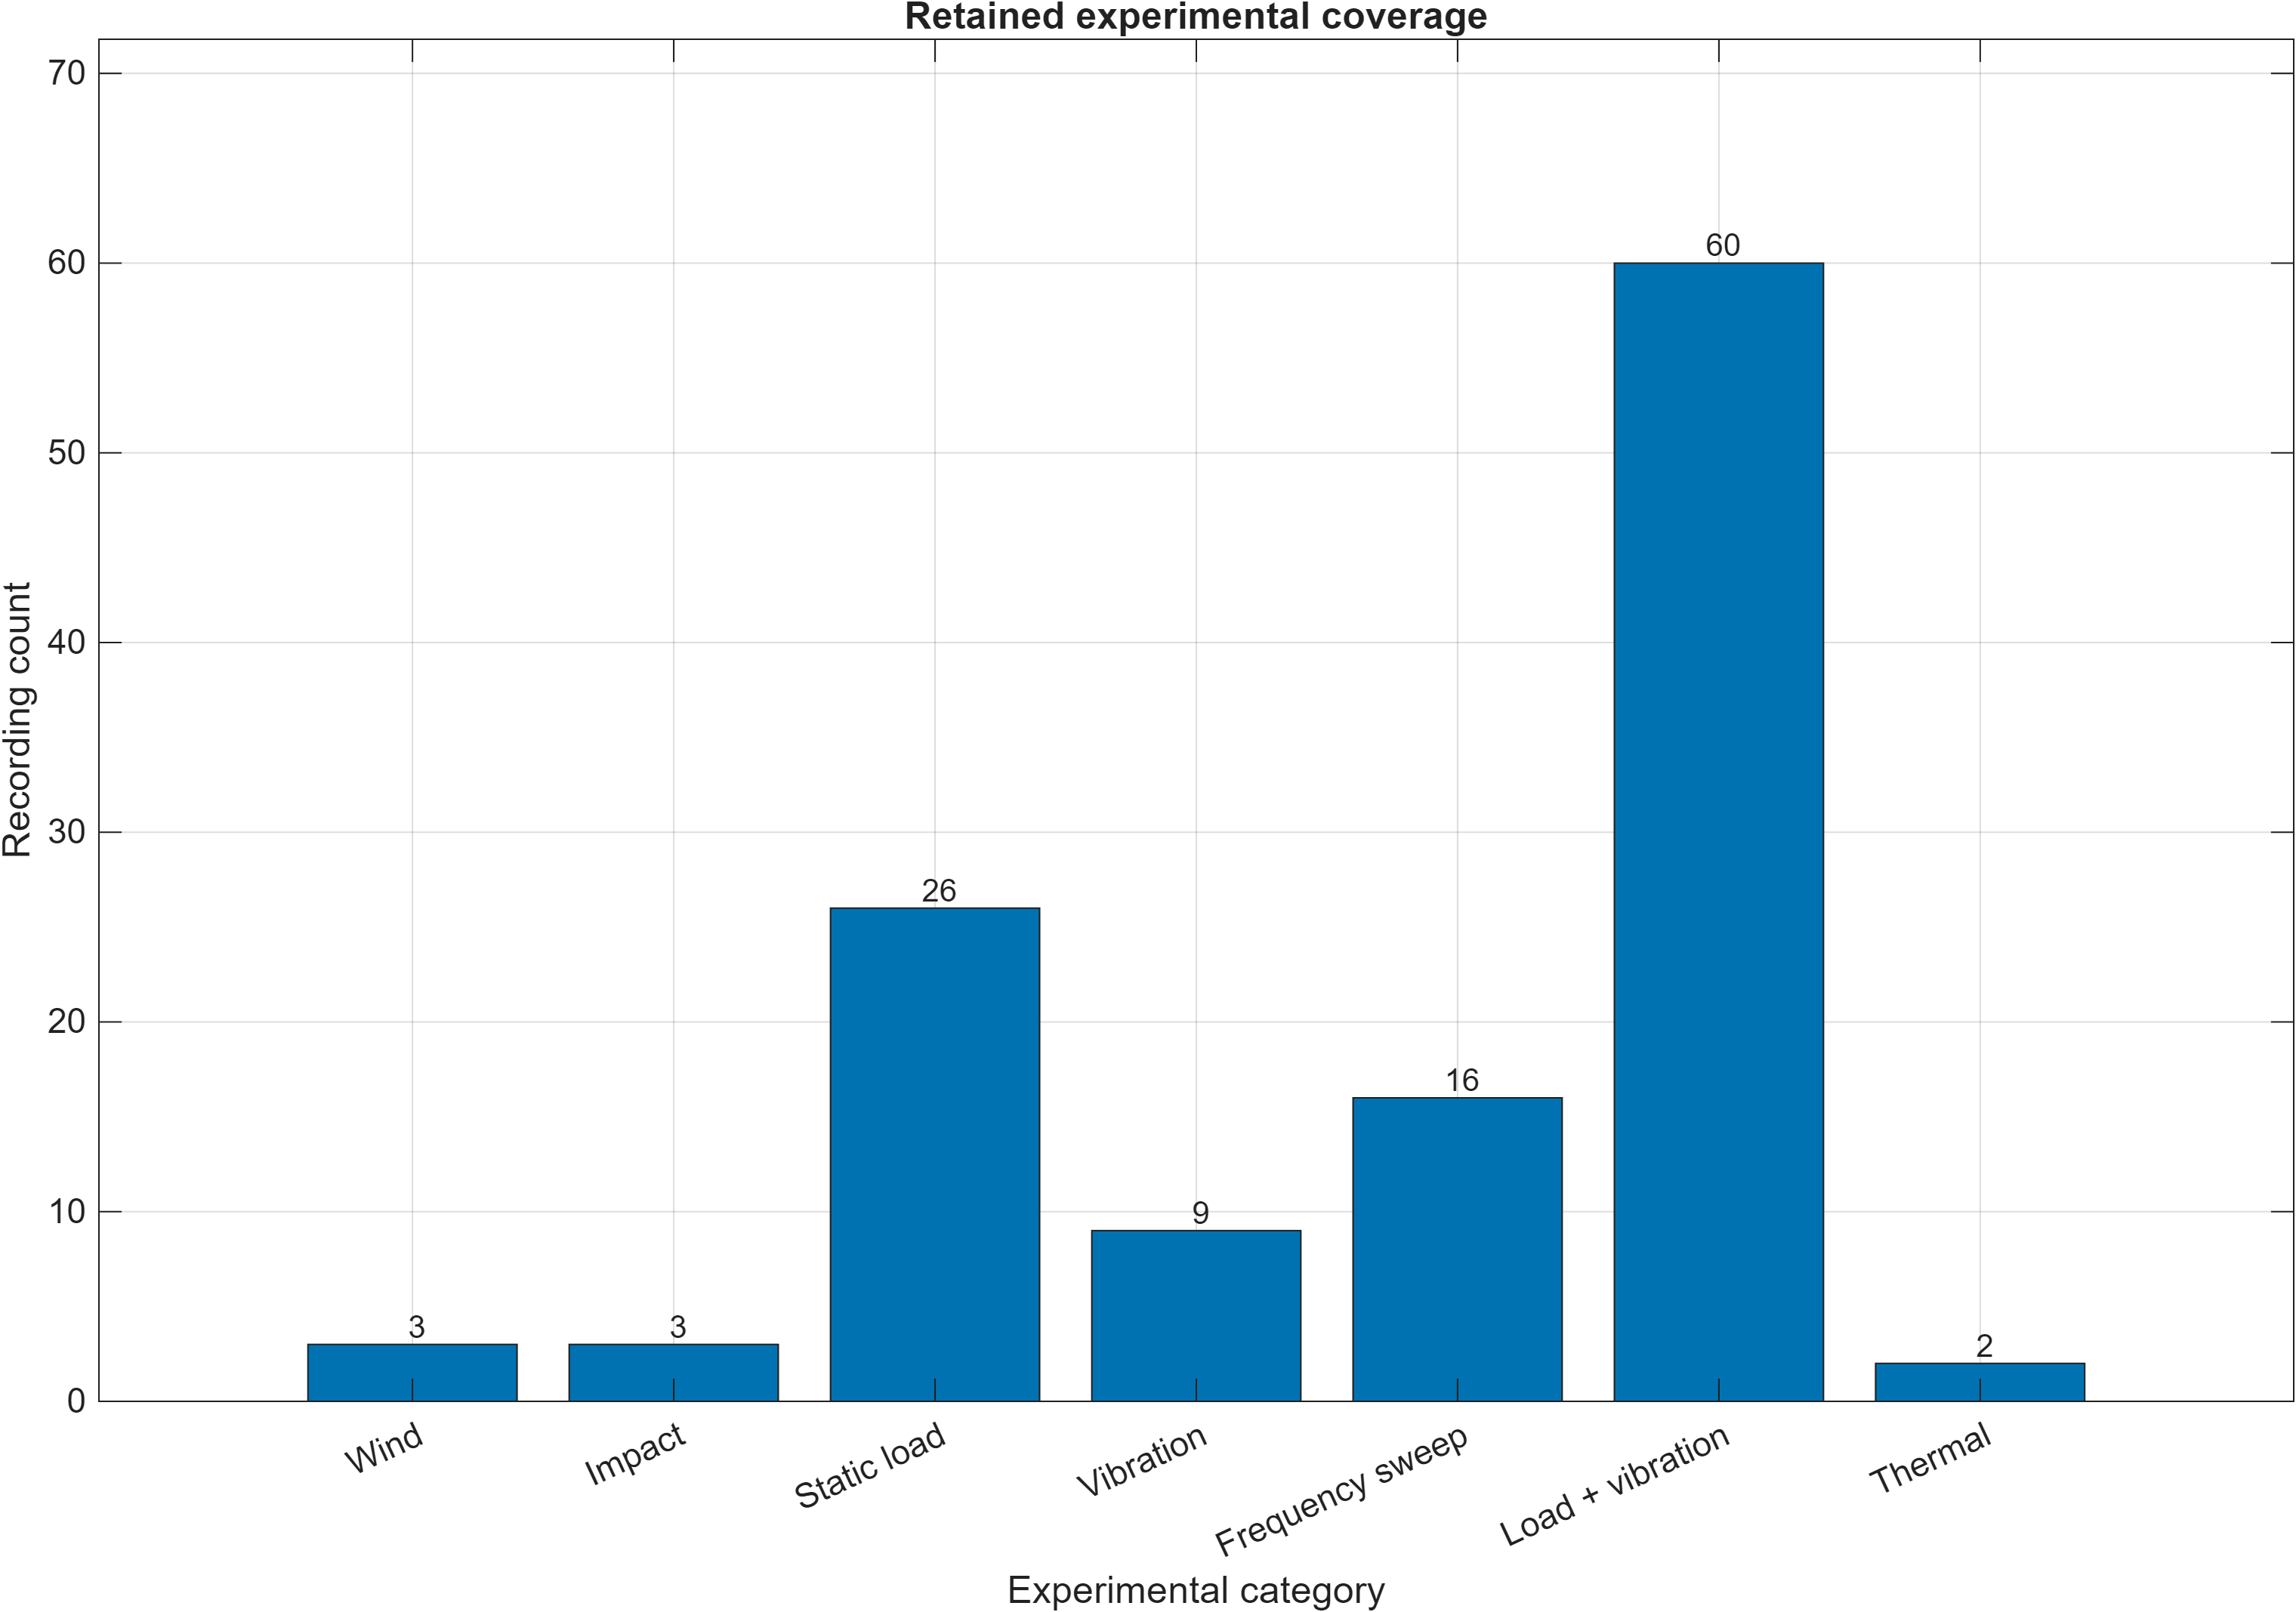
\includegraphics[width=\textwidth,height=0.37\textheight,keepaspectratio]{figures/F01_experimental_categories.png}
\caption{Counts of cleaned recordings by experimental category.}\label{fig:F01}
\end{figure}
Combined load/vibration dominates the retained design: 60 of 119 recordings (50.4 percent), compared with 26 static and 9 unloaded-vibration runs. This balance supports condition-specific comparisons but gives greater descriptive weight to the combined campaign. The two thermal files represent one interrupted session, not replication of environmental behavior. Coverage therefore supports identifying candidate sensor-response relationships; it does not establish a balanced validation dataset or justify pooling acquisition batches.\par

\renewcommand{\thefigure}{F02}
\begin{figure}[H]\centering
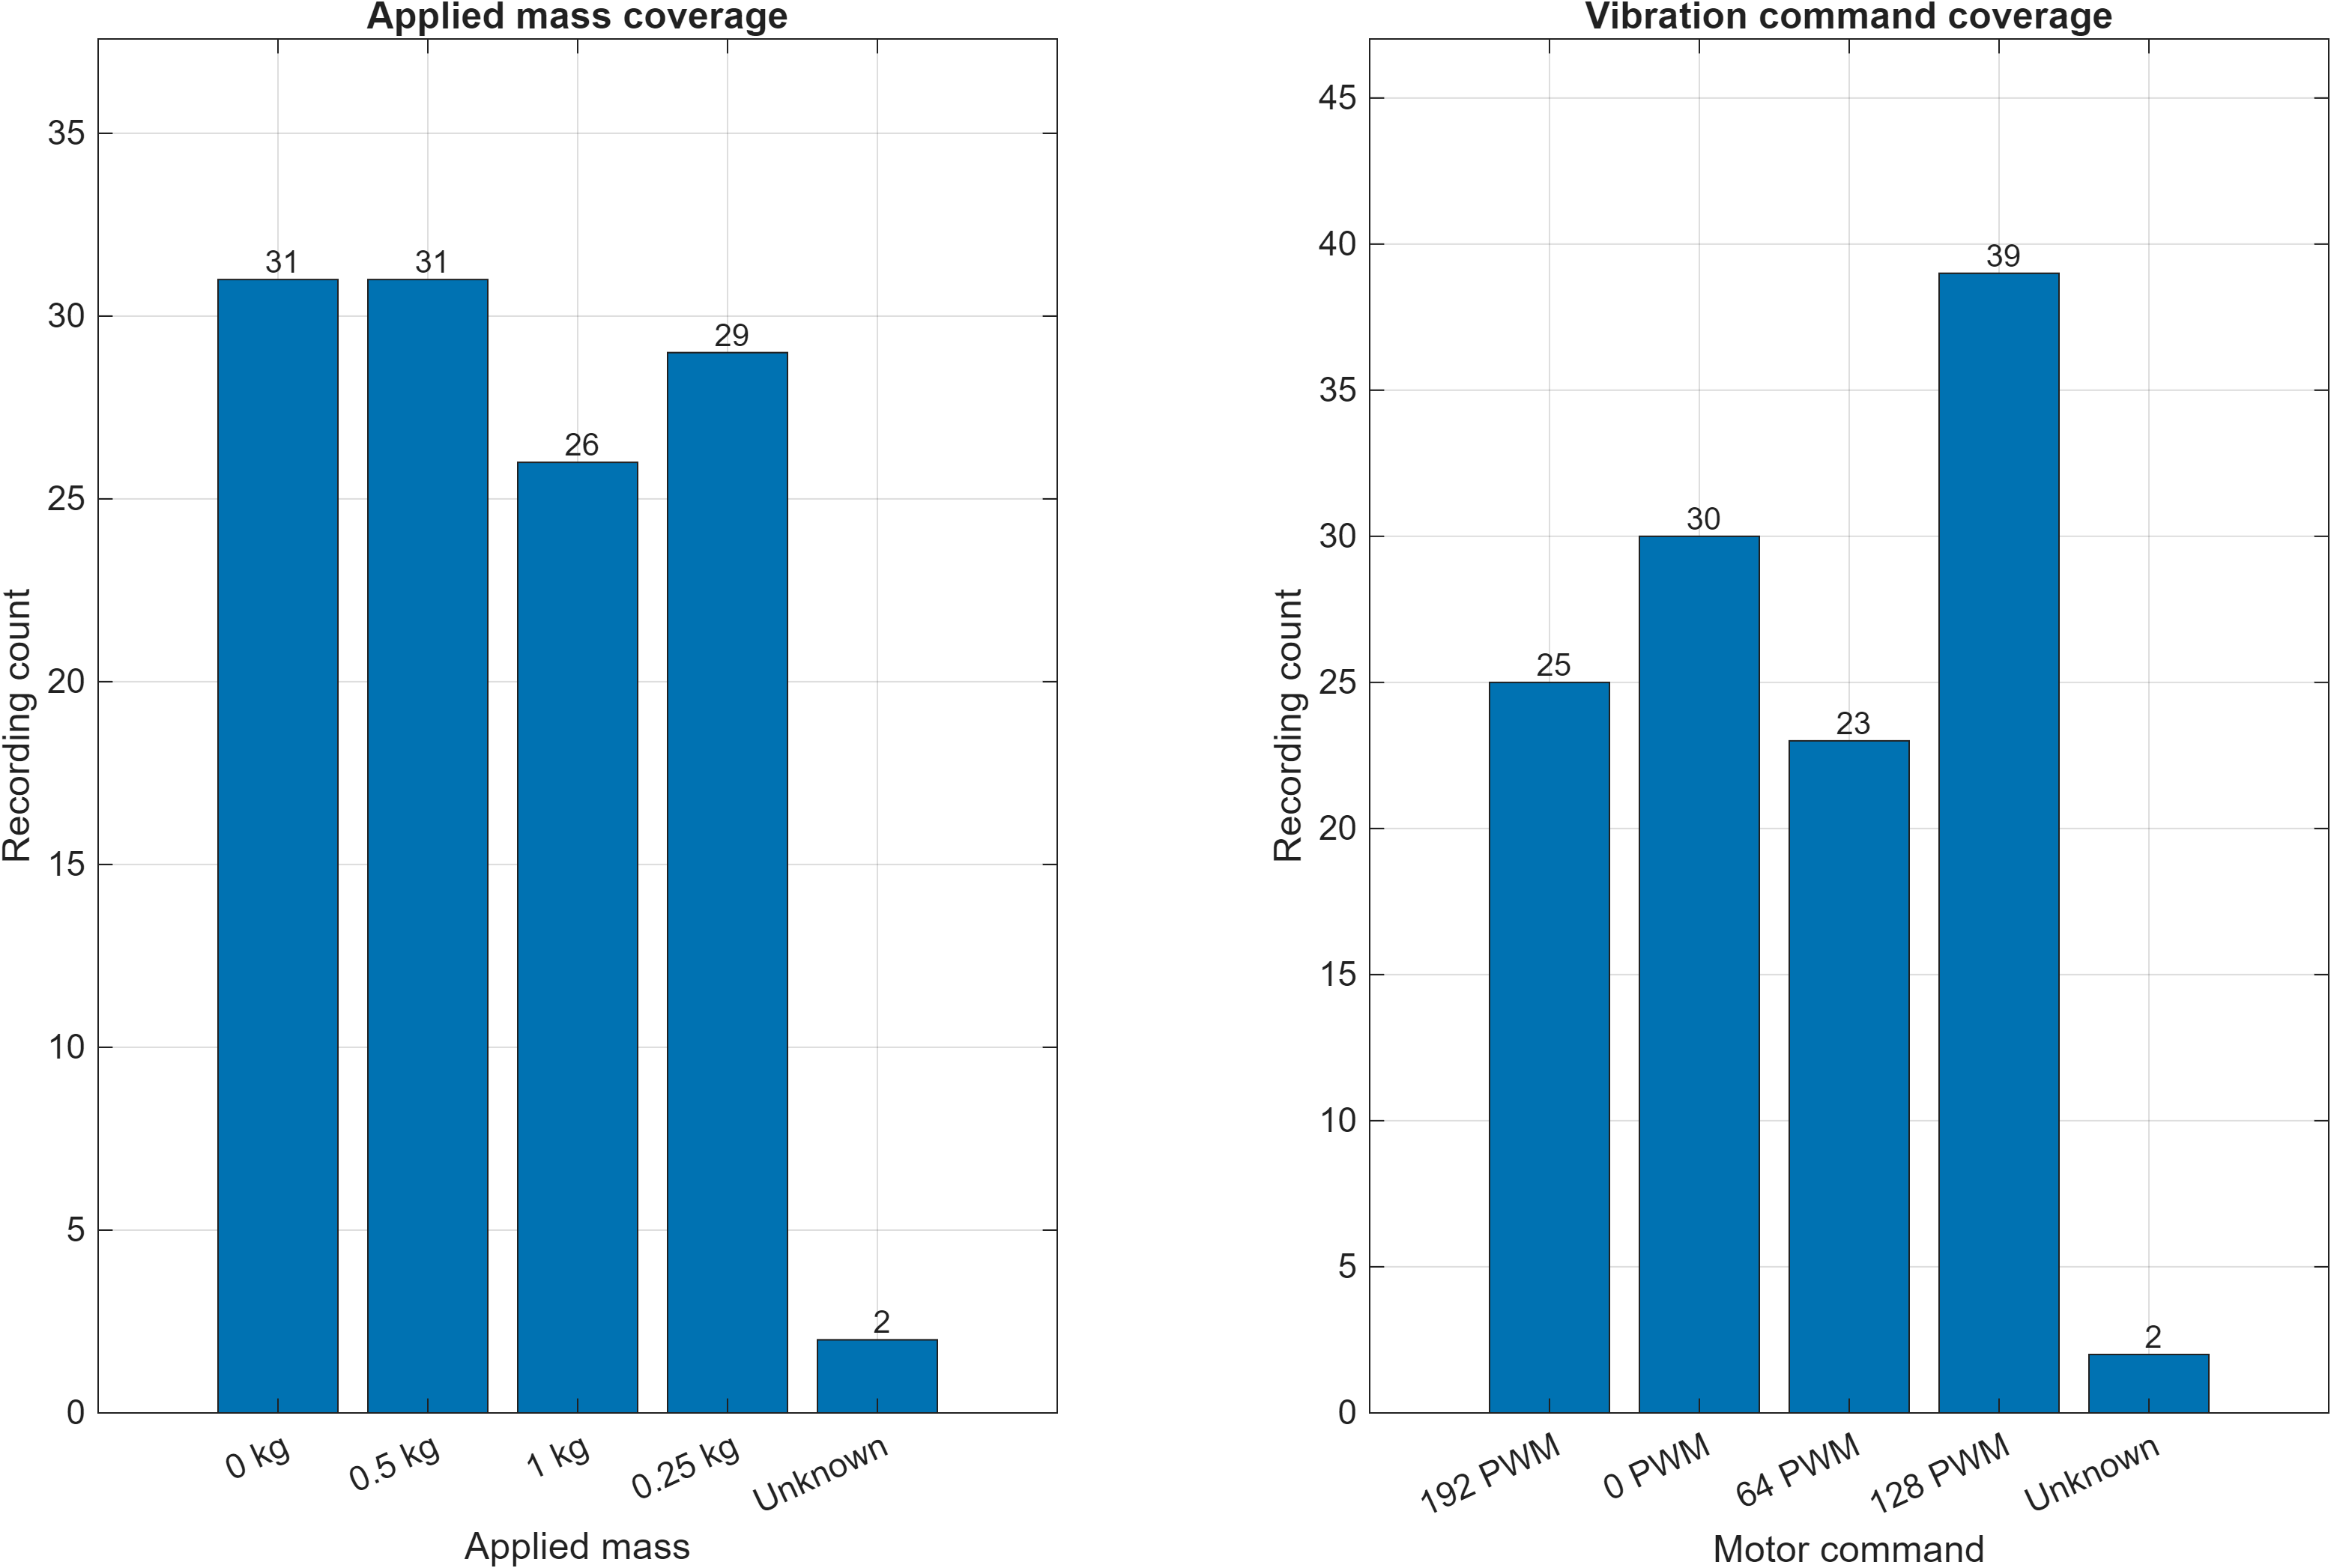
\includegraphics[width=\textwidth,height=0.37\textheight,keepaspectratio]{figures/F02_condition_counts.png}
\caption{Coverage of applied mass and motor PWM, including explicit unknown values.}\label{fig:F02}
\end{figure}
Known mass and PWM metadata are present for 117 recordings; 2 thermal segments remain explicitly unknown. PWM 192 has 25 recordings, versus 23 at PWM 64. These are acquisition counts, not evidence of stronger excitation or better repeatability. Since the mass, position and motor settings are not equally represented, an unstratified average would mix operating conditions and batch effects. Later response comparisons therefore retain matched conditions.\par

\renewcommand{\thefigure}{F03}
\begin{figure}[H]\centering
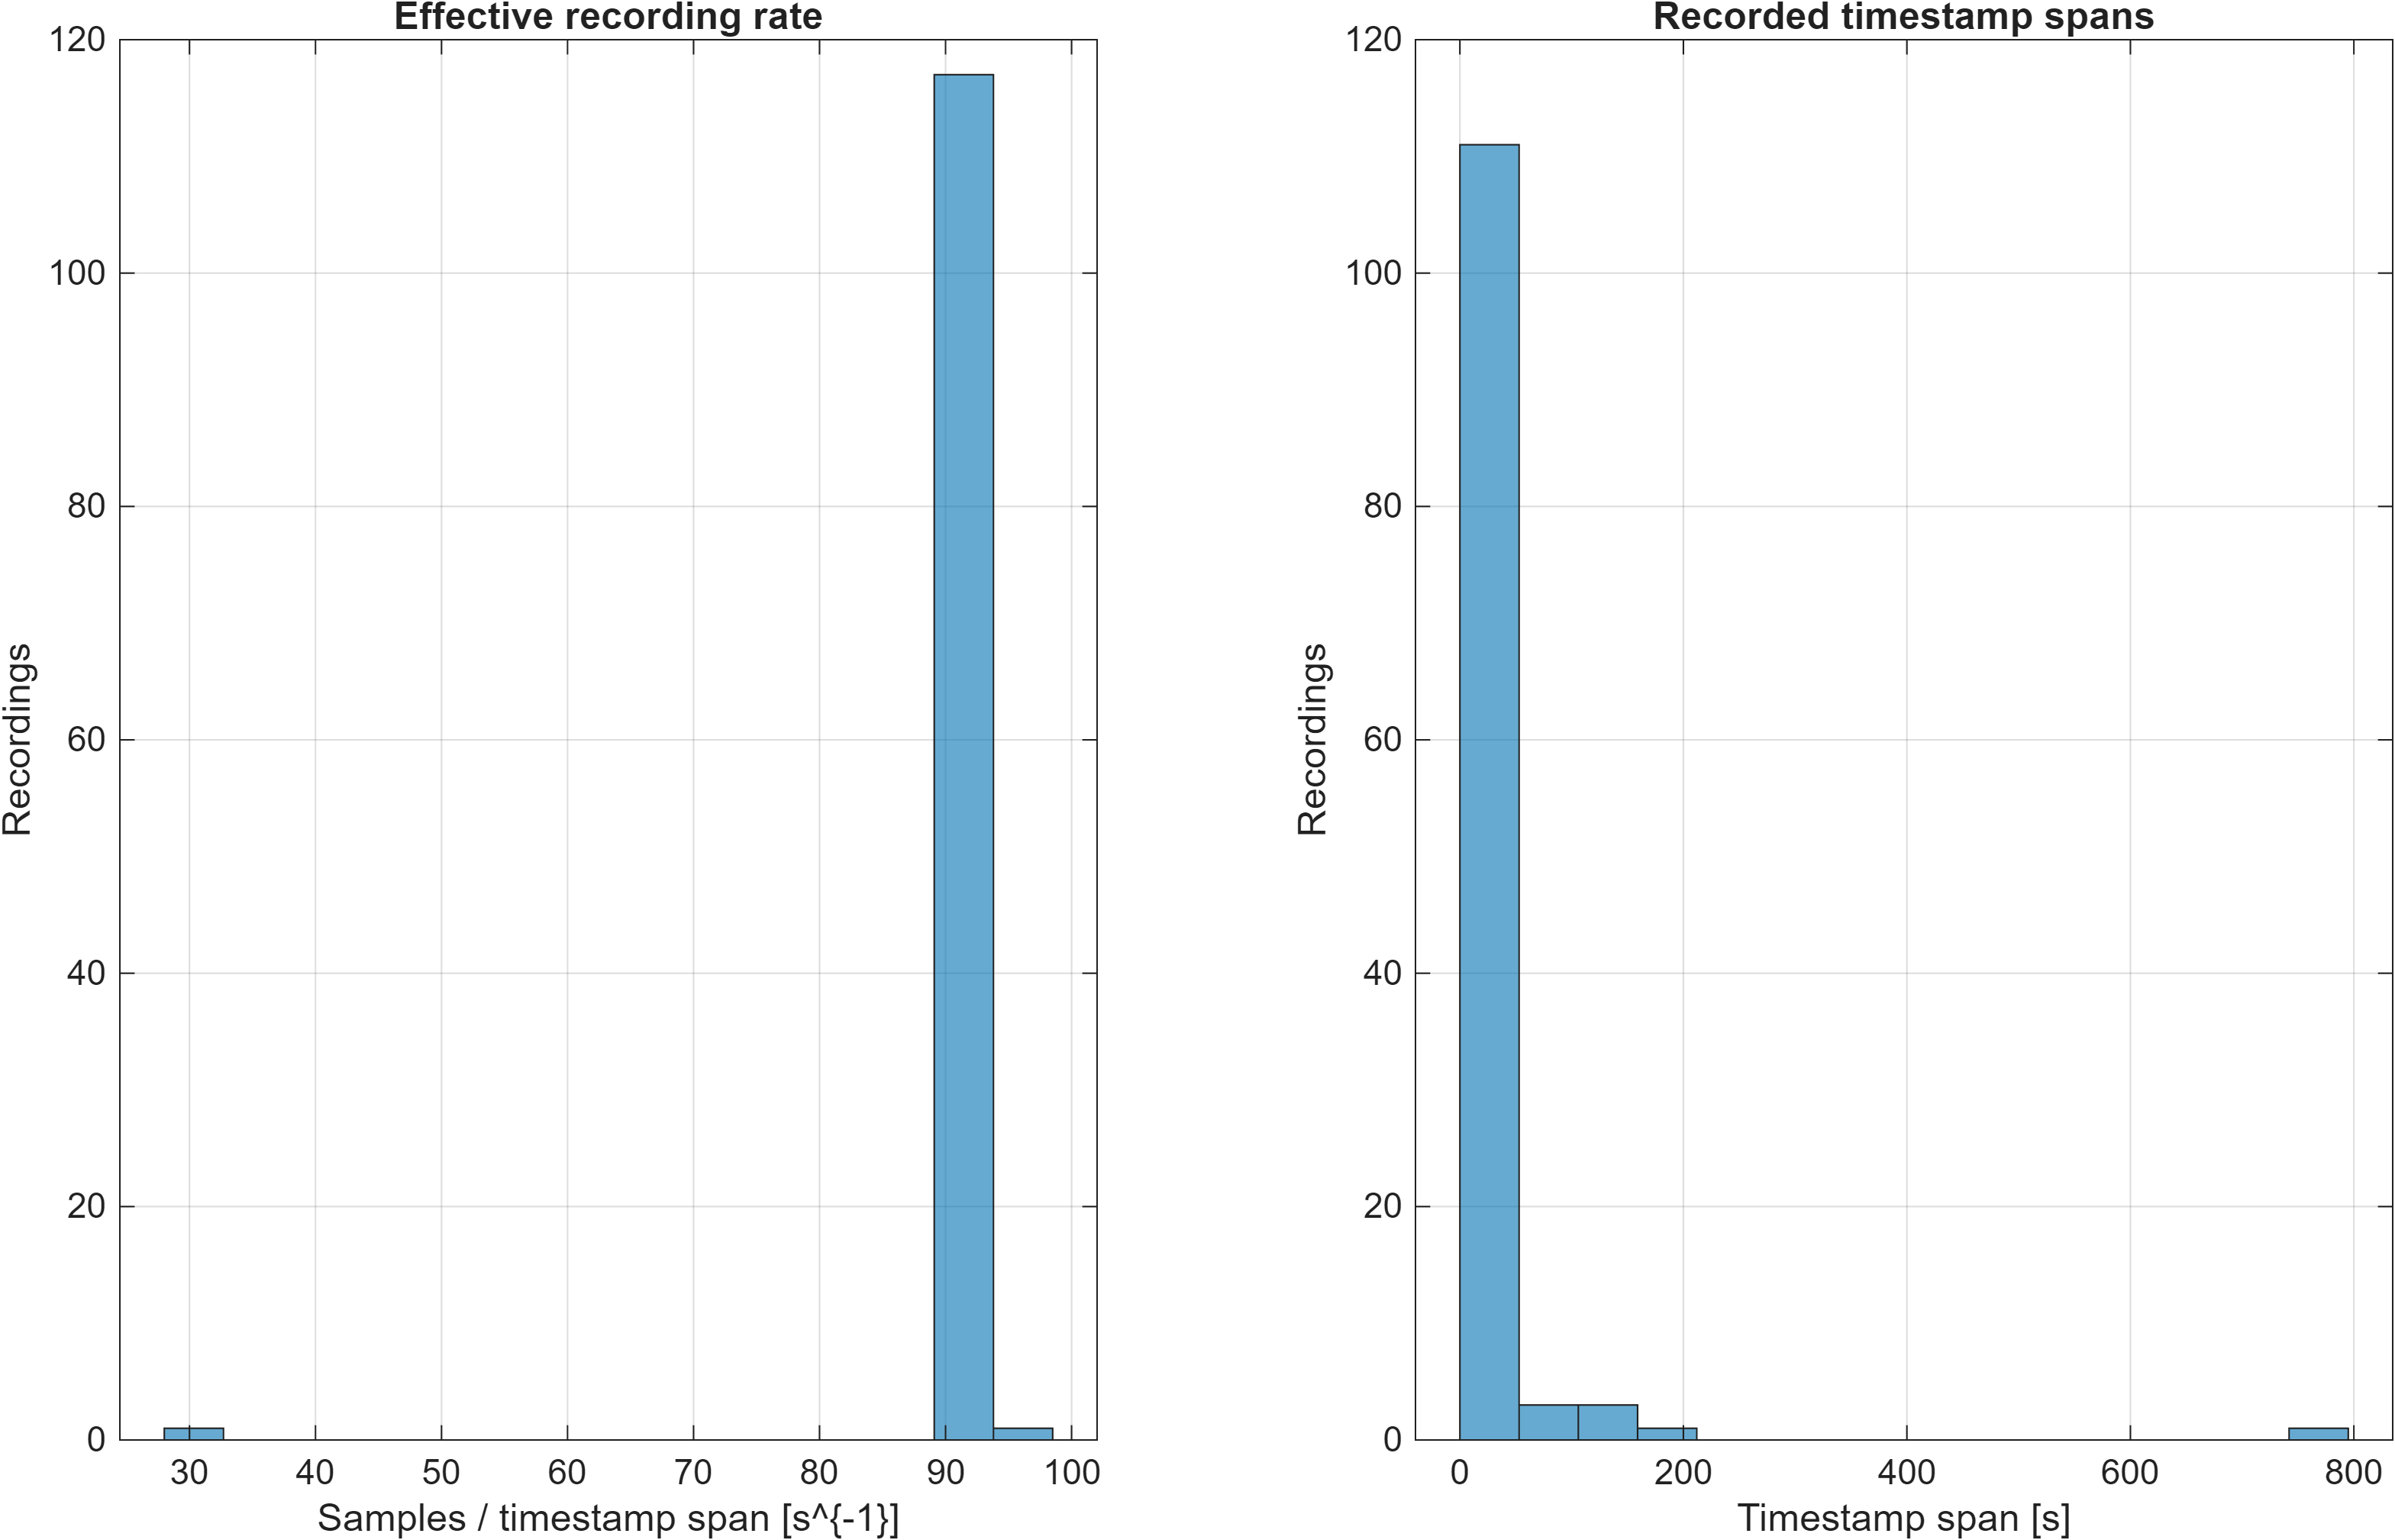
\includegraphics[width=\textwidth,height=0.37\textheight,keepaspectratio]{figures/F03_timing_distributions.png}
\caption{Effective sample rate and timestamp-span distributions.}\label{fig:F03}
\end{figure}
The median timestamp increment suggests 100.000 Hz, but the median effective recording rate is only 90.944 samples/s: gaps reduce temporal coverage despite a nominally fast clock. Thermal segment 2 is the strongest duration anomaly, with a 785.919 s timestamp span but only 246.093 s between finite sensor endpoints. Its leading missing interval depresses the effective rate and must not be interpreted as measured slow sampling. Neither histogram alone establishes FFT eligibility; continuity is audited separately.\par

\renewcommand{\thefigure}{F04}
\begin{figure}[H]\centering
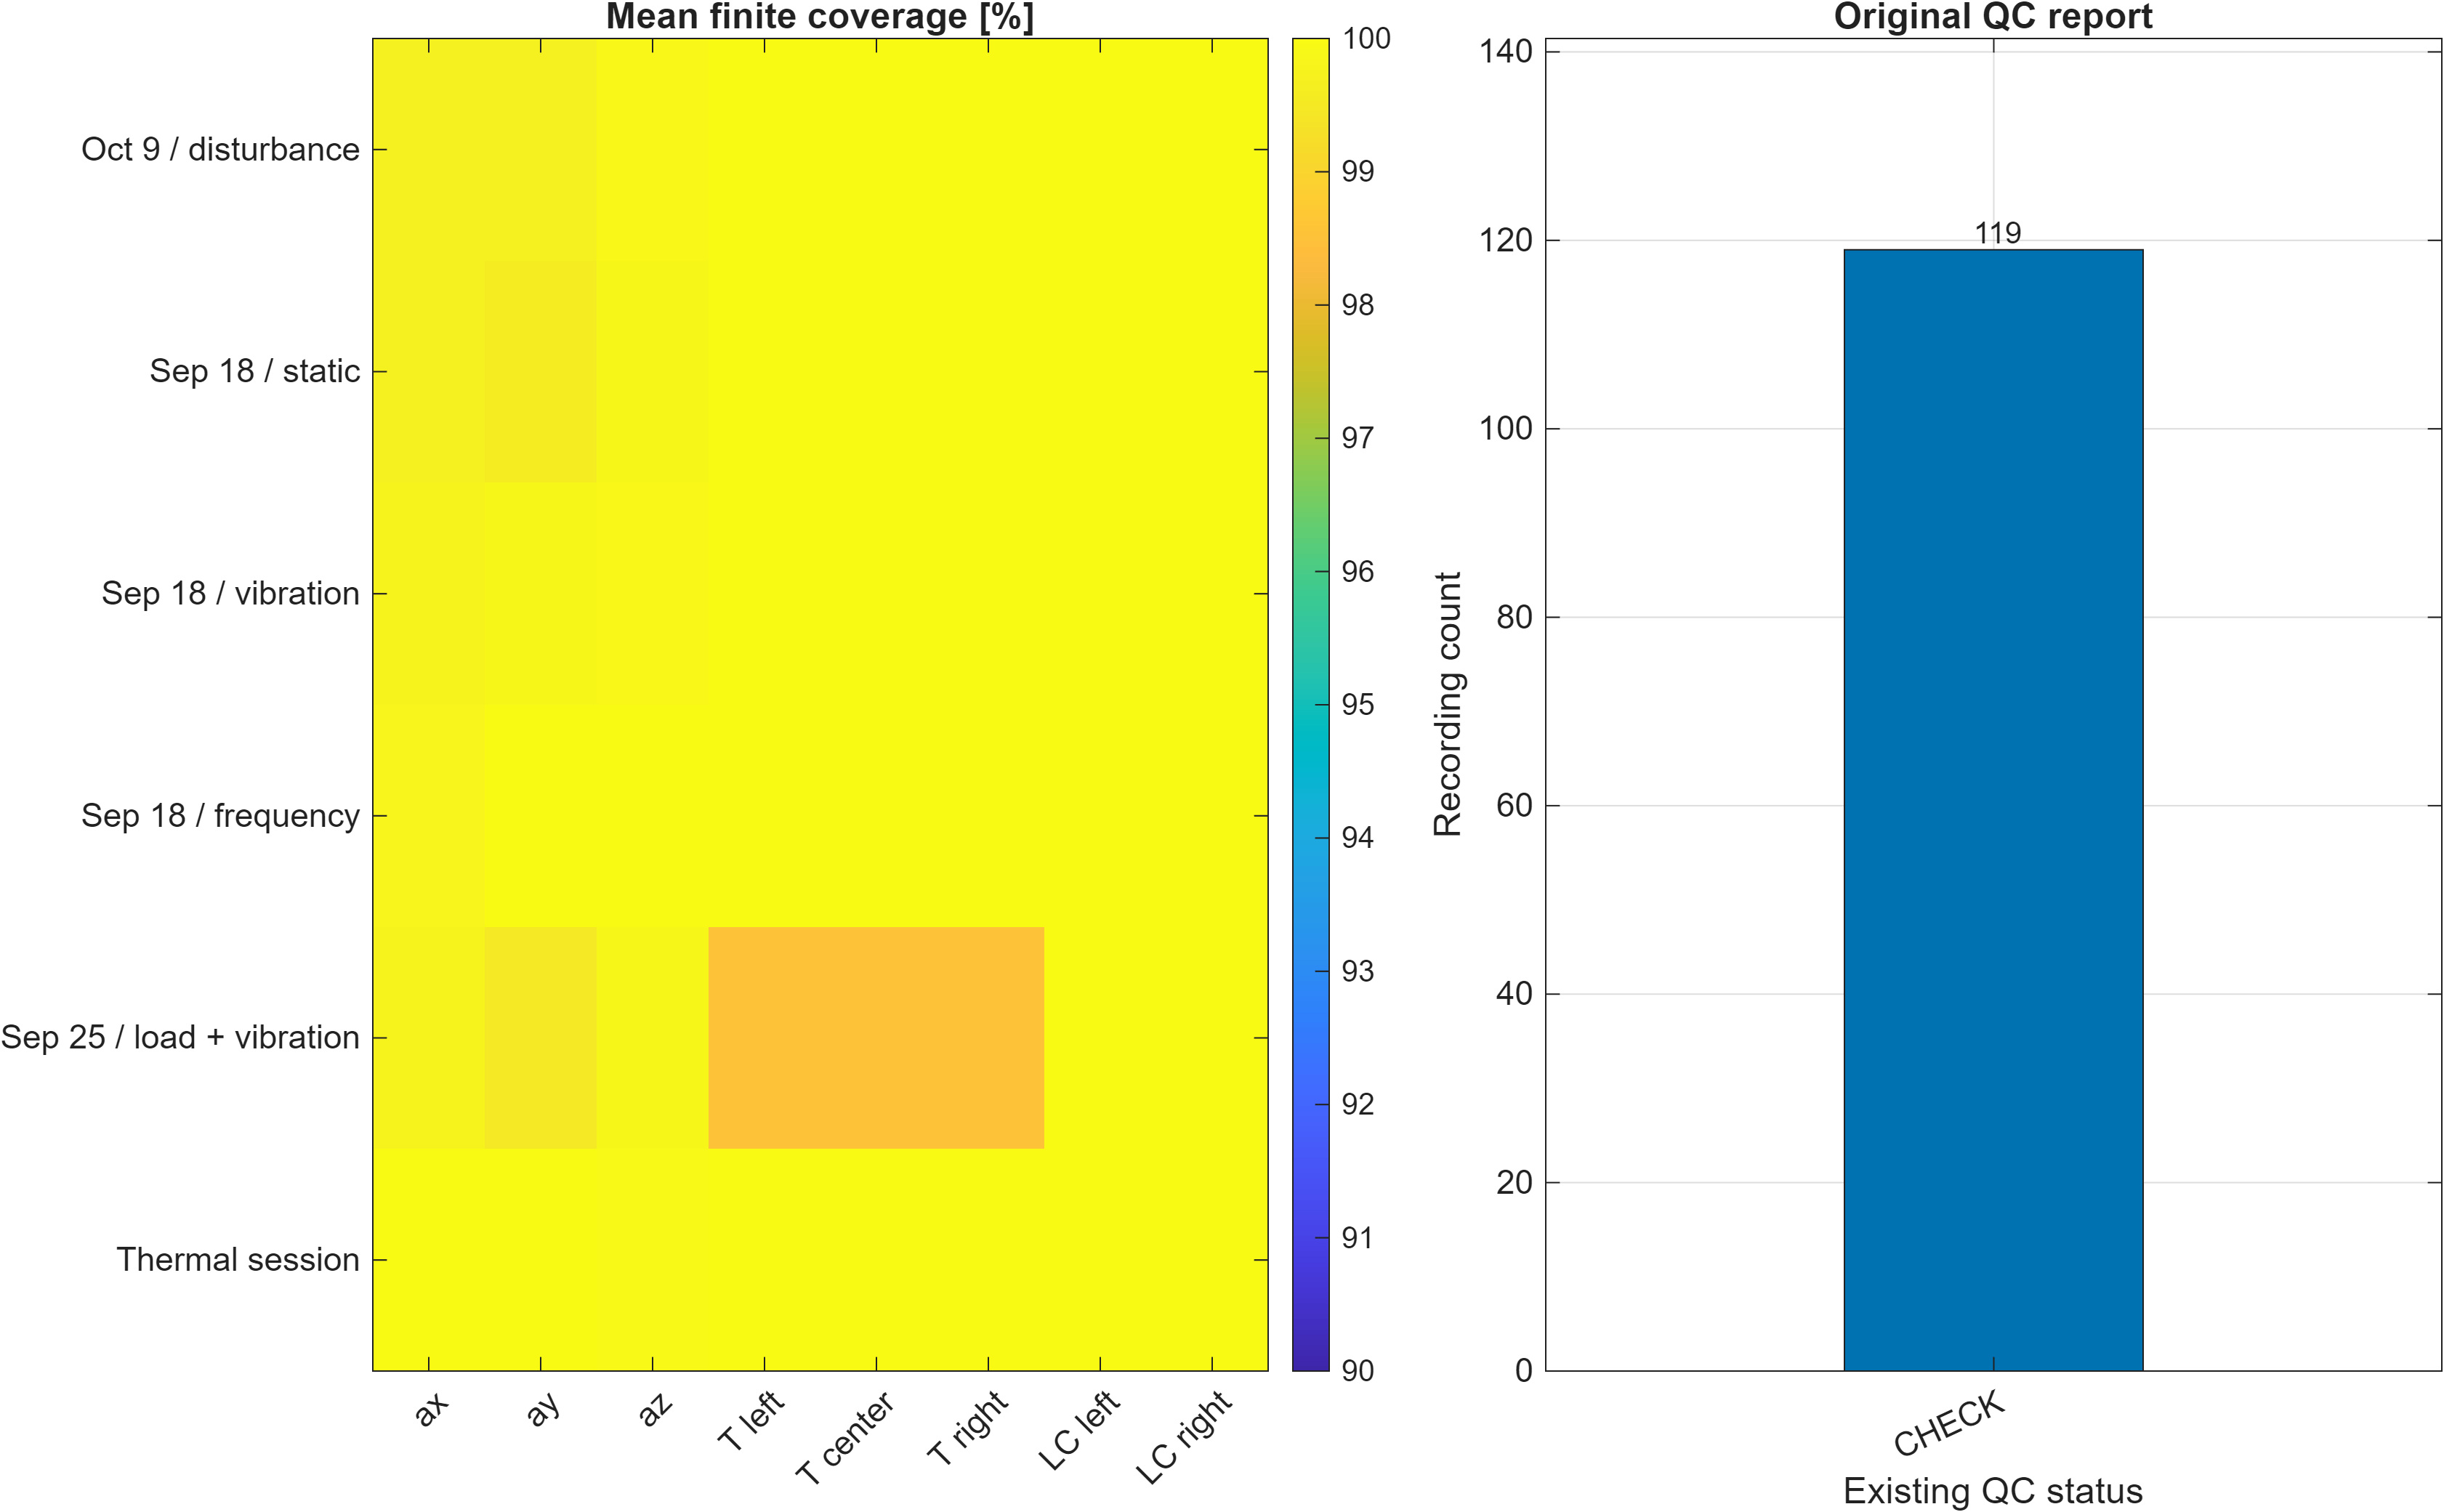
\includegraphics[width=\textwidth,height=0.37\textheight,keepaspectratio]{figures/F04_sensor_coverage_qc.png}
\caption{Finite sensor coverage by batch and unchanged source QC status.}\label{fig:F04}
\end{figure}
High average coverage conceals a complete channel loss: T0236 contains 3302 samples but no finite values in any of its three temperature channels. Its valid acceleration cannot restore the missing environmental context. All 119 retained recordings carry CHECK status, so coverage is not equivalent to accepted measurement quality. Missing channels and timestamp gaps require separate controls; the recovered T0236 spectrum remains useful only as a conditional acceleration observation, without a simultaneous temperature comparison.\par

\Needspace{5\baselineskip}
\section{Static Load Characterization}
Static recordings quantify the measured load-cell response to applied mass. The 0.25 kg runs were acquired on September 25, whereas the retained 0.5 and 1 kg static series were acquired on September 18. These batches are not combined into a single calibration curve. Individual repetitions and raw signal asymmetry expose variability without asserting that an expected mechanical trend occurred.

\renewcommand{\thefigure}{F05}
\begin{figure}[H]\centering
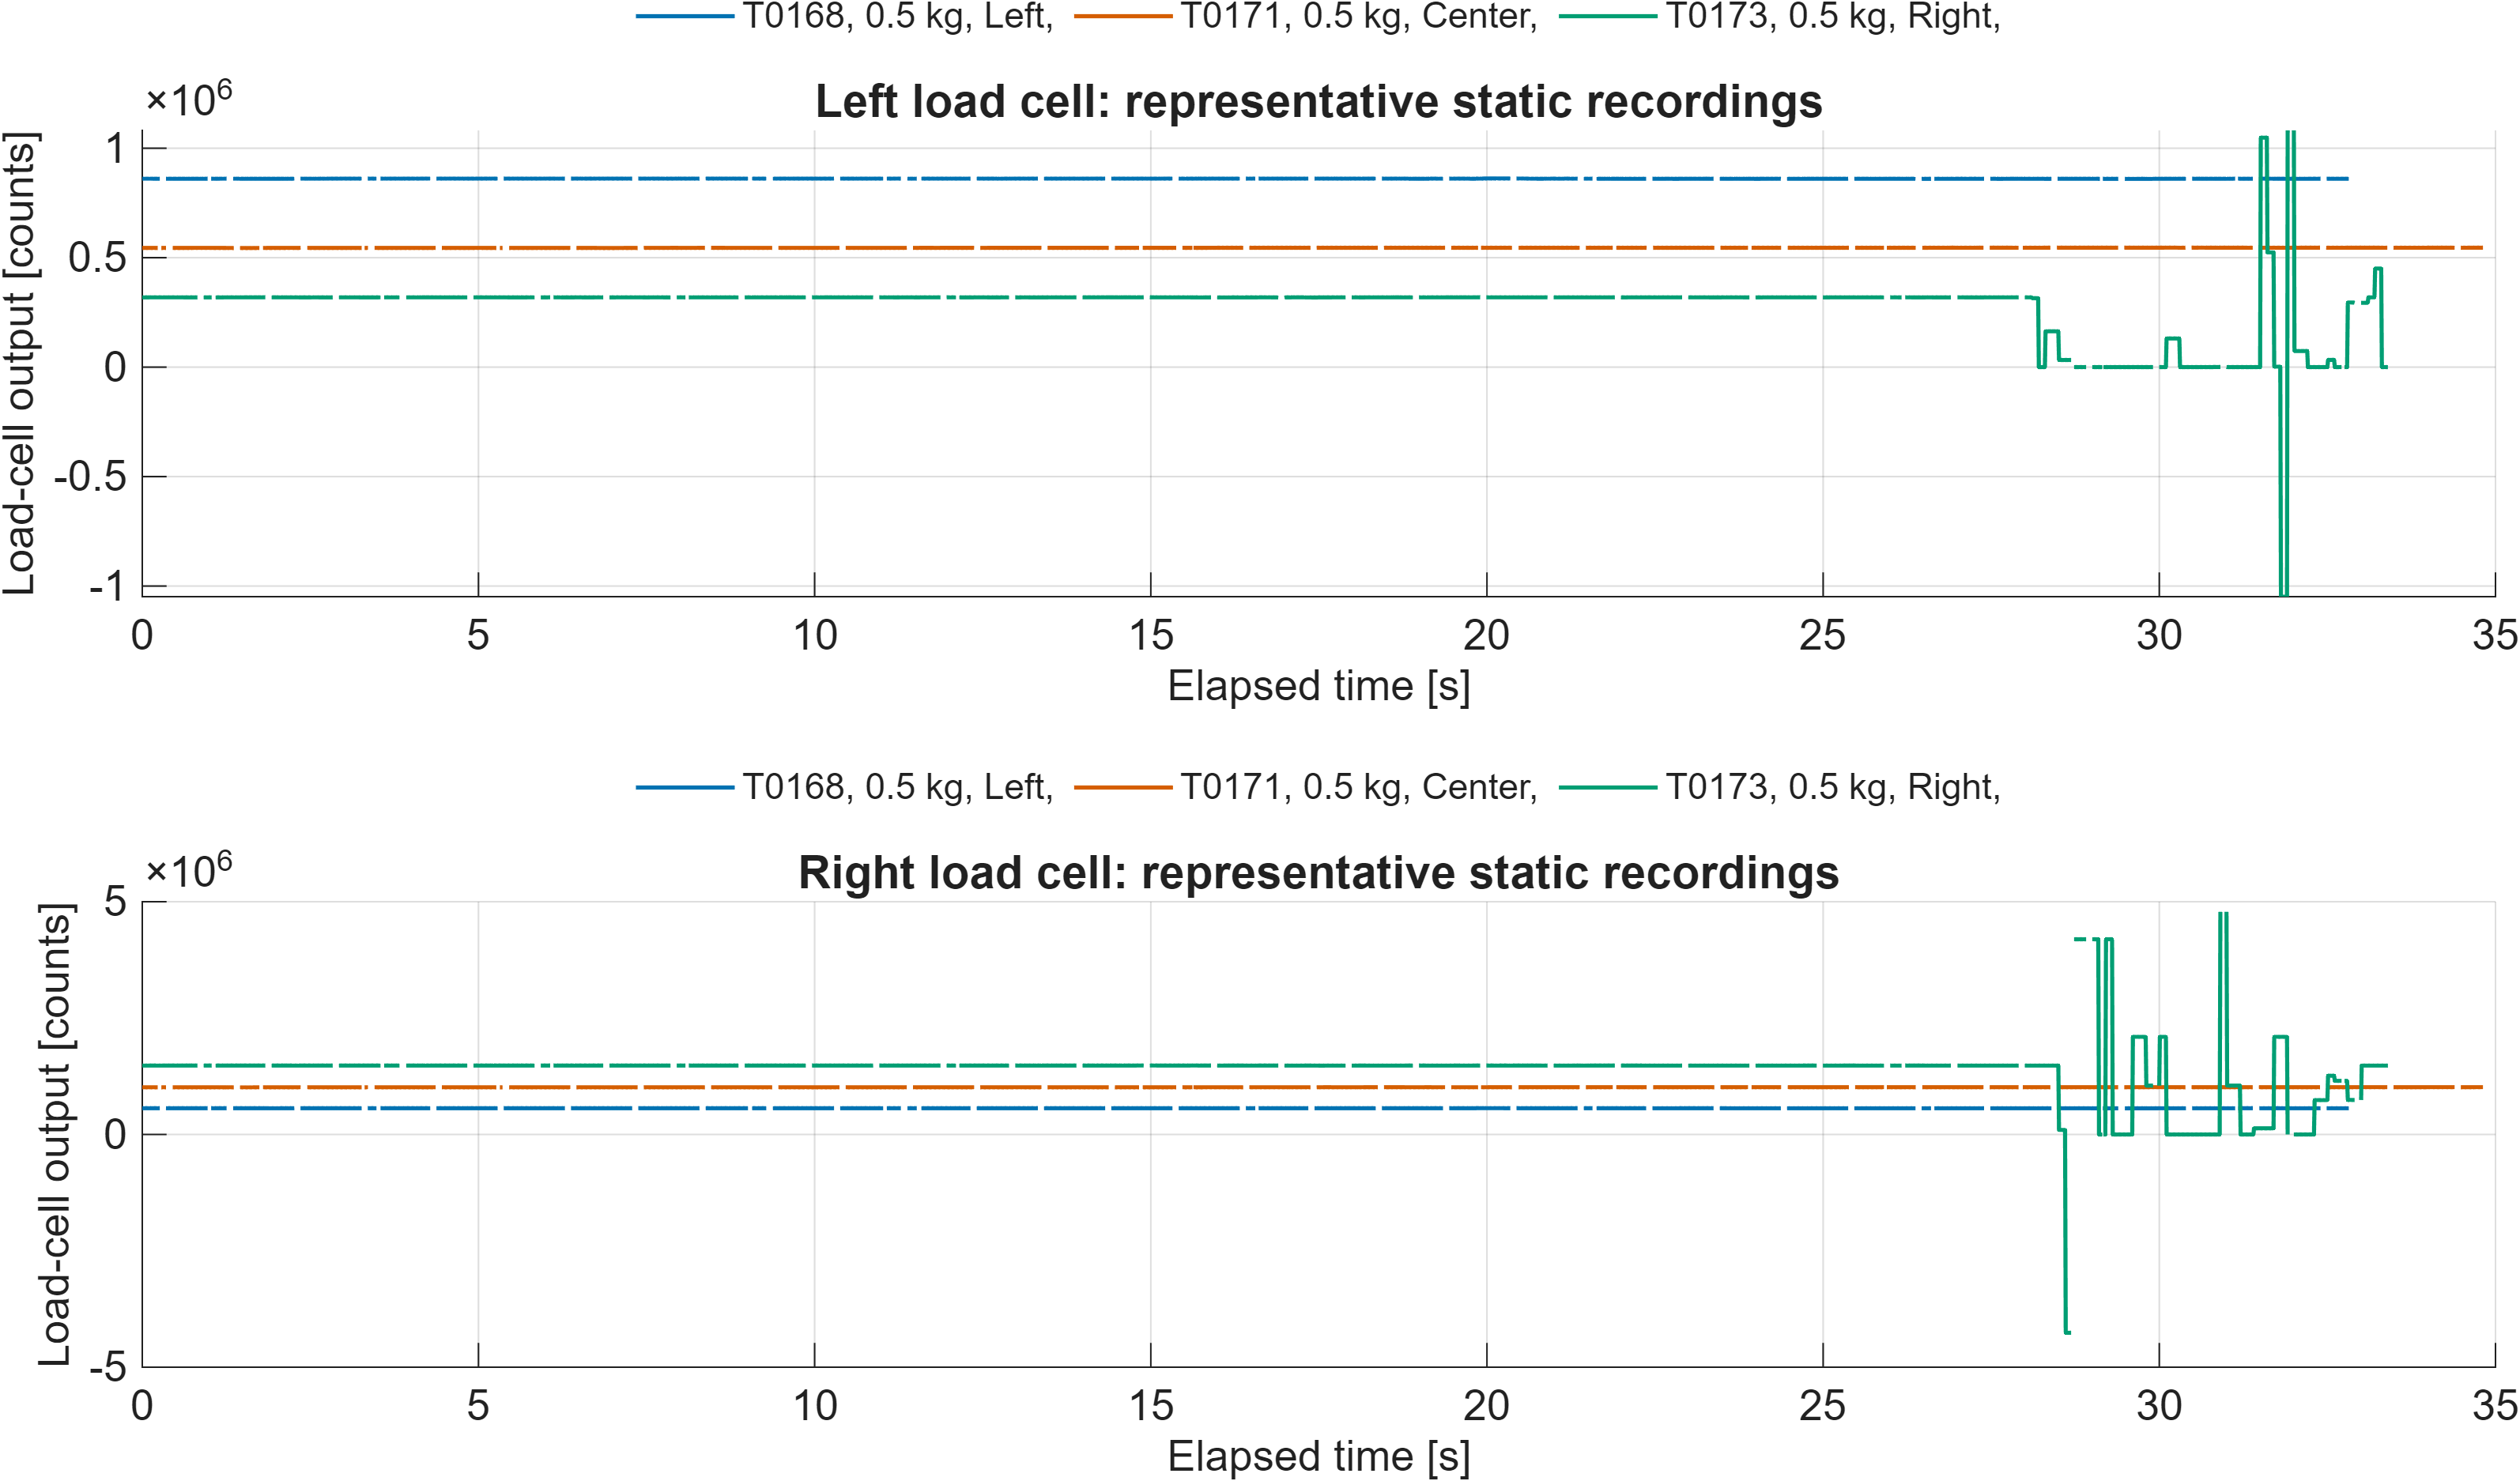
\includegraphics[width=\textwidth,height=0.37\textheight,keepaspectratio]{figures/F05_static_time_histories.png}
\caption{Representative static load-cell time histories by position.}\label{fig:F05}
\end{figure}
At the same 0.5 kg mass, the representative left-cell medians decrease from 861032 counts under left loading to 318913 under right loading, while the opposite channel increases. This is consistent with location-dependent transfer through the bridge and supports using both channels to distinguish position. However, T0173 also contains abrupt late-record changes: its right-channel maximum-minus-minimum span is 9043967 counts. Such excursions are not explained by a static mass label and could reflect load movement, mounting changes or acquisition artifacts. The stable portions and run medians should therefore not be taken as proof that the entire waveform is trustworthy. A synchronized loading log and calibrated channels are needed to separate mechanical response from measurement faults.\par

\renewcommand{\thefigure}{F06}
\begin{figure}[H]\centering
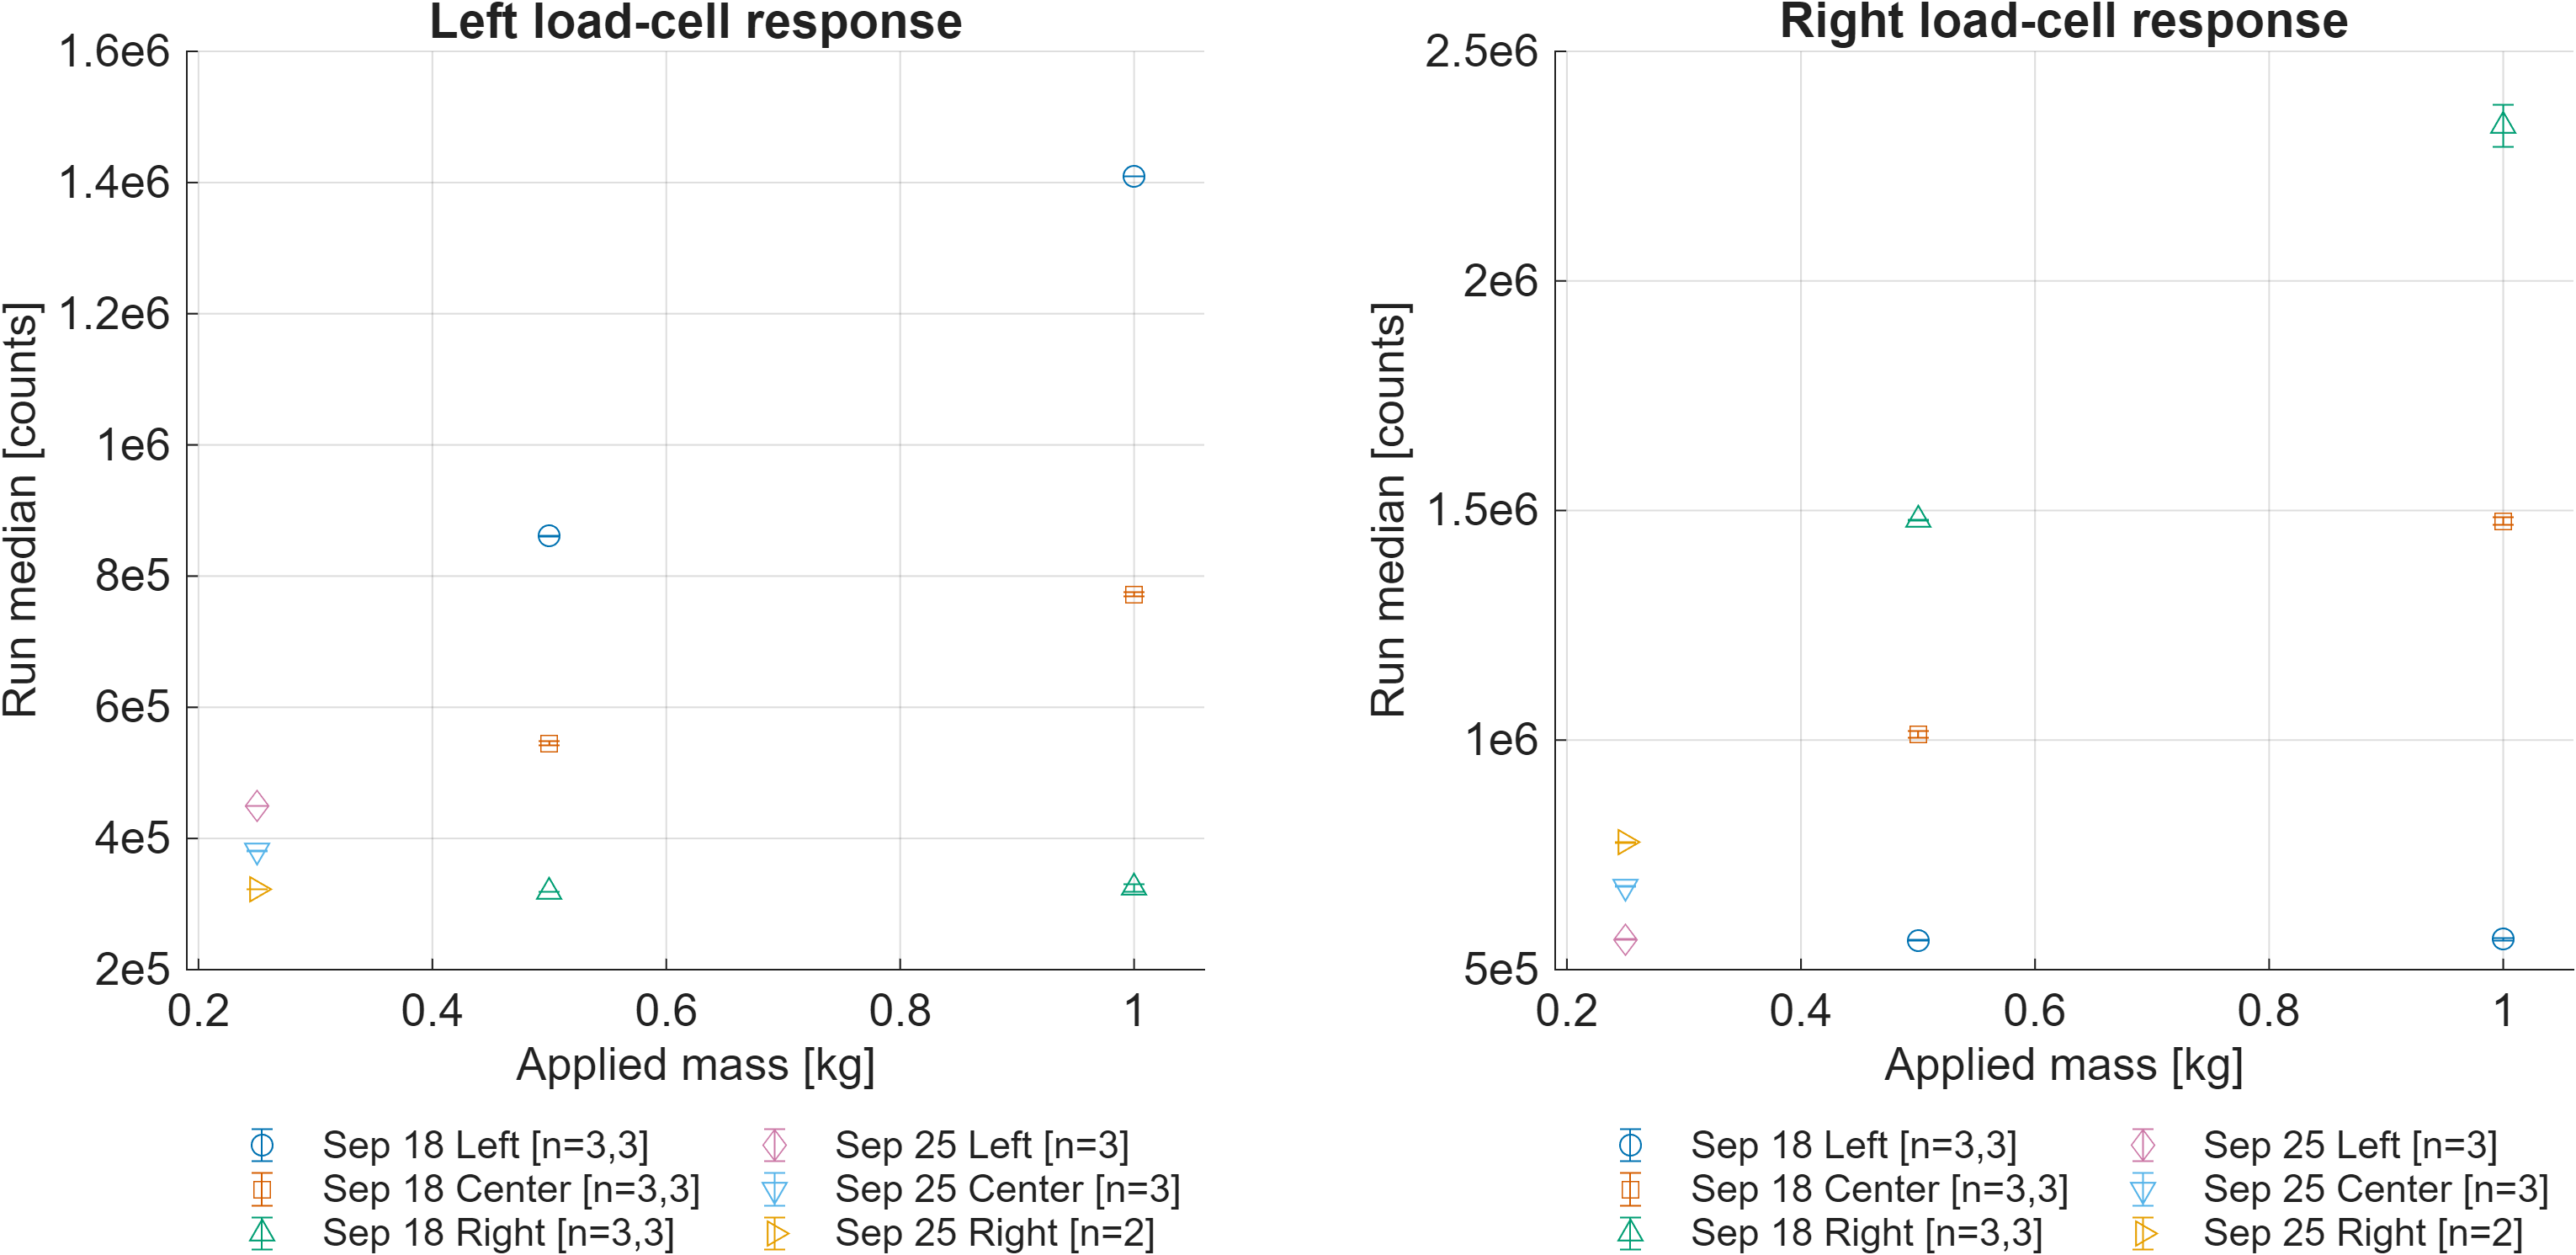
\includegraphics[width=\textwidth,height=0.37\textheight,keepaspectratio]{figures/F06_static_mass_response.png}
\caption{Run-median load-cell output versus applied mass, separated by batch and position.}\label{fig:F06}
\end{figure}
Doubling applied mass from 0.5 to 1 kg produces strongly position-dependent count changes within September 18. Left-cell means of run medians rise 63.7 percent for left loading and 41.6 percent at center, but only 1.79 percent for right loading. Conversely, the right-cell change is only 0.34 percent under left loading and 58.0 percent under right loading. Thus both channels increase over the two tested mass levels, but their sensitivities are far from interchangeable. A nearby load path and channel-specific offsets or gains could produce this pattern; it is not a calibrated force distribution. The separate September 25 0.25 kg series cannot establish a common linear calibration, and two mass levels cannot establish general linearity.\par

\renewcommand{\thefigure}{F07}
\begin{figure}[H]\centering
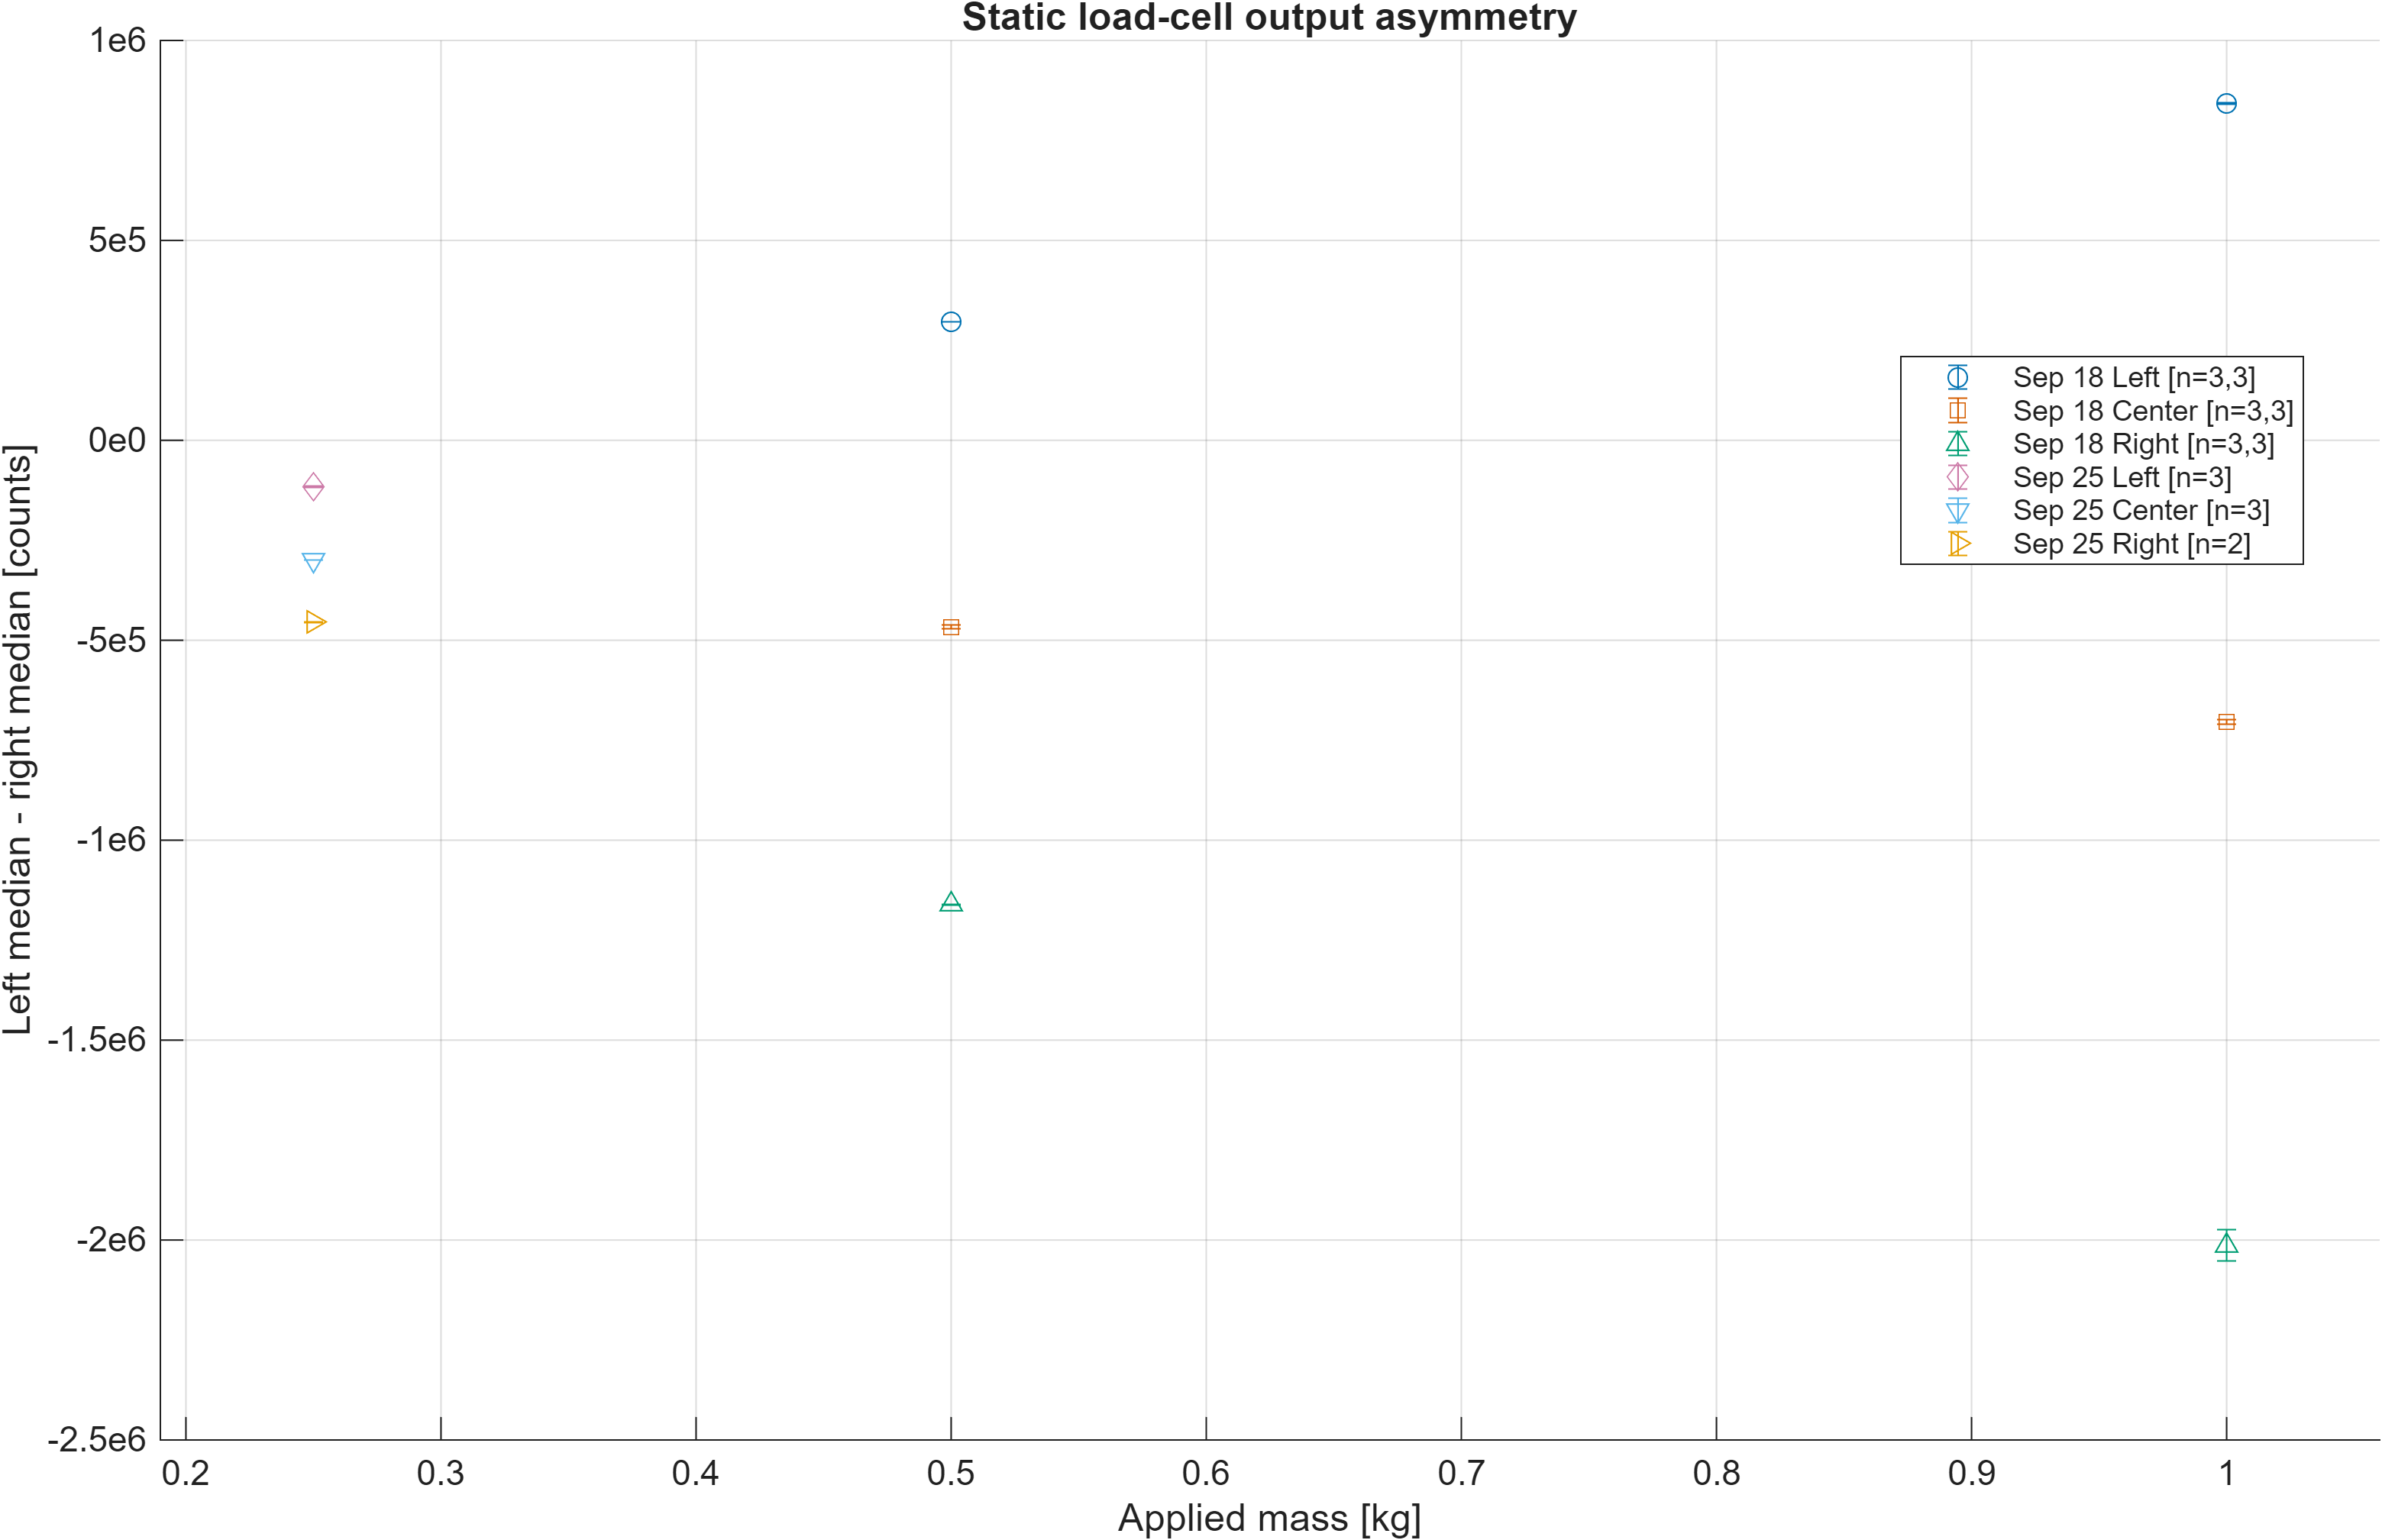
\includegraphics[width=\textwidth,height=0.37\textheight,keepaspectratio]{figures/F07_static_asymmetry.png}
\caption{Difference between left and right run-median load-cell outputs.}\label{fig:F07}
\end{figure}
Output asymmetry is not a universal monotonic function of mass. When mass doubles, left-minus-right counts increase by 546294 under left loading, but decrease by 237490 at center and 852575 under right loading. The direction depends on which channel acquires the larger incremental response. This supports treating mass and position jointly in a future measurement model, rather than using a single pooled asymmetry-to-mass curve. The center value remains negative at both masses, showing that a centered load does not zero this uncalibrated difference. Unequal channel offsets, gains and mounting compliance are plausible contributors. Without tare and independent calibration, neither the sign nor its magnitude quantifies unequal support forces.\par

\renewcommand{\thefigure}{F08}
\begin{figure}[H]\centering
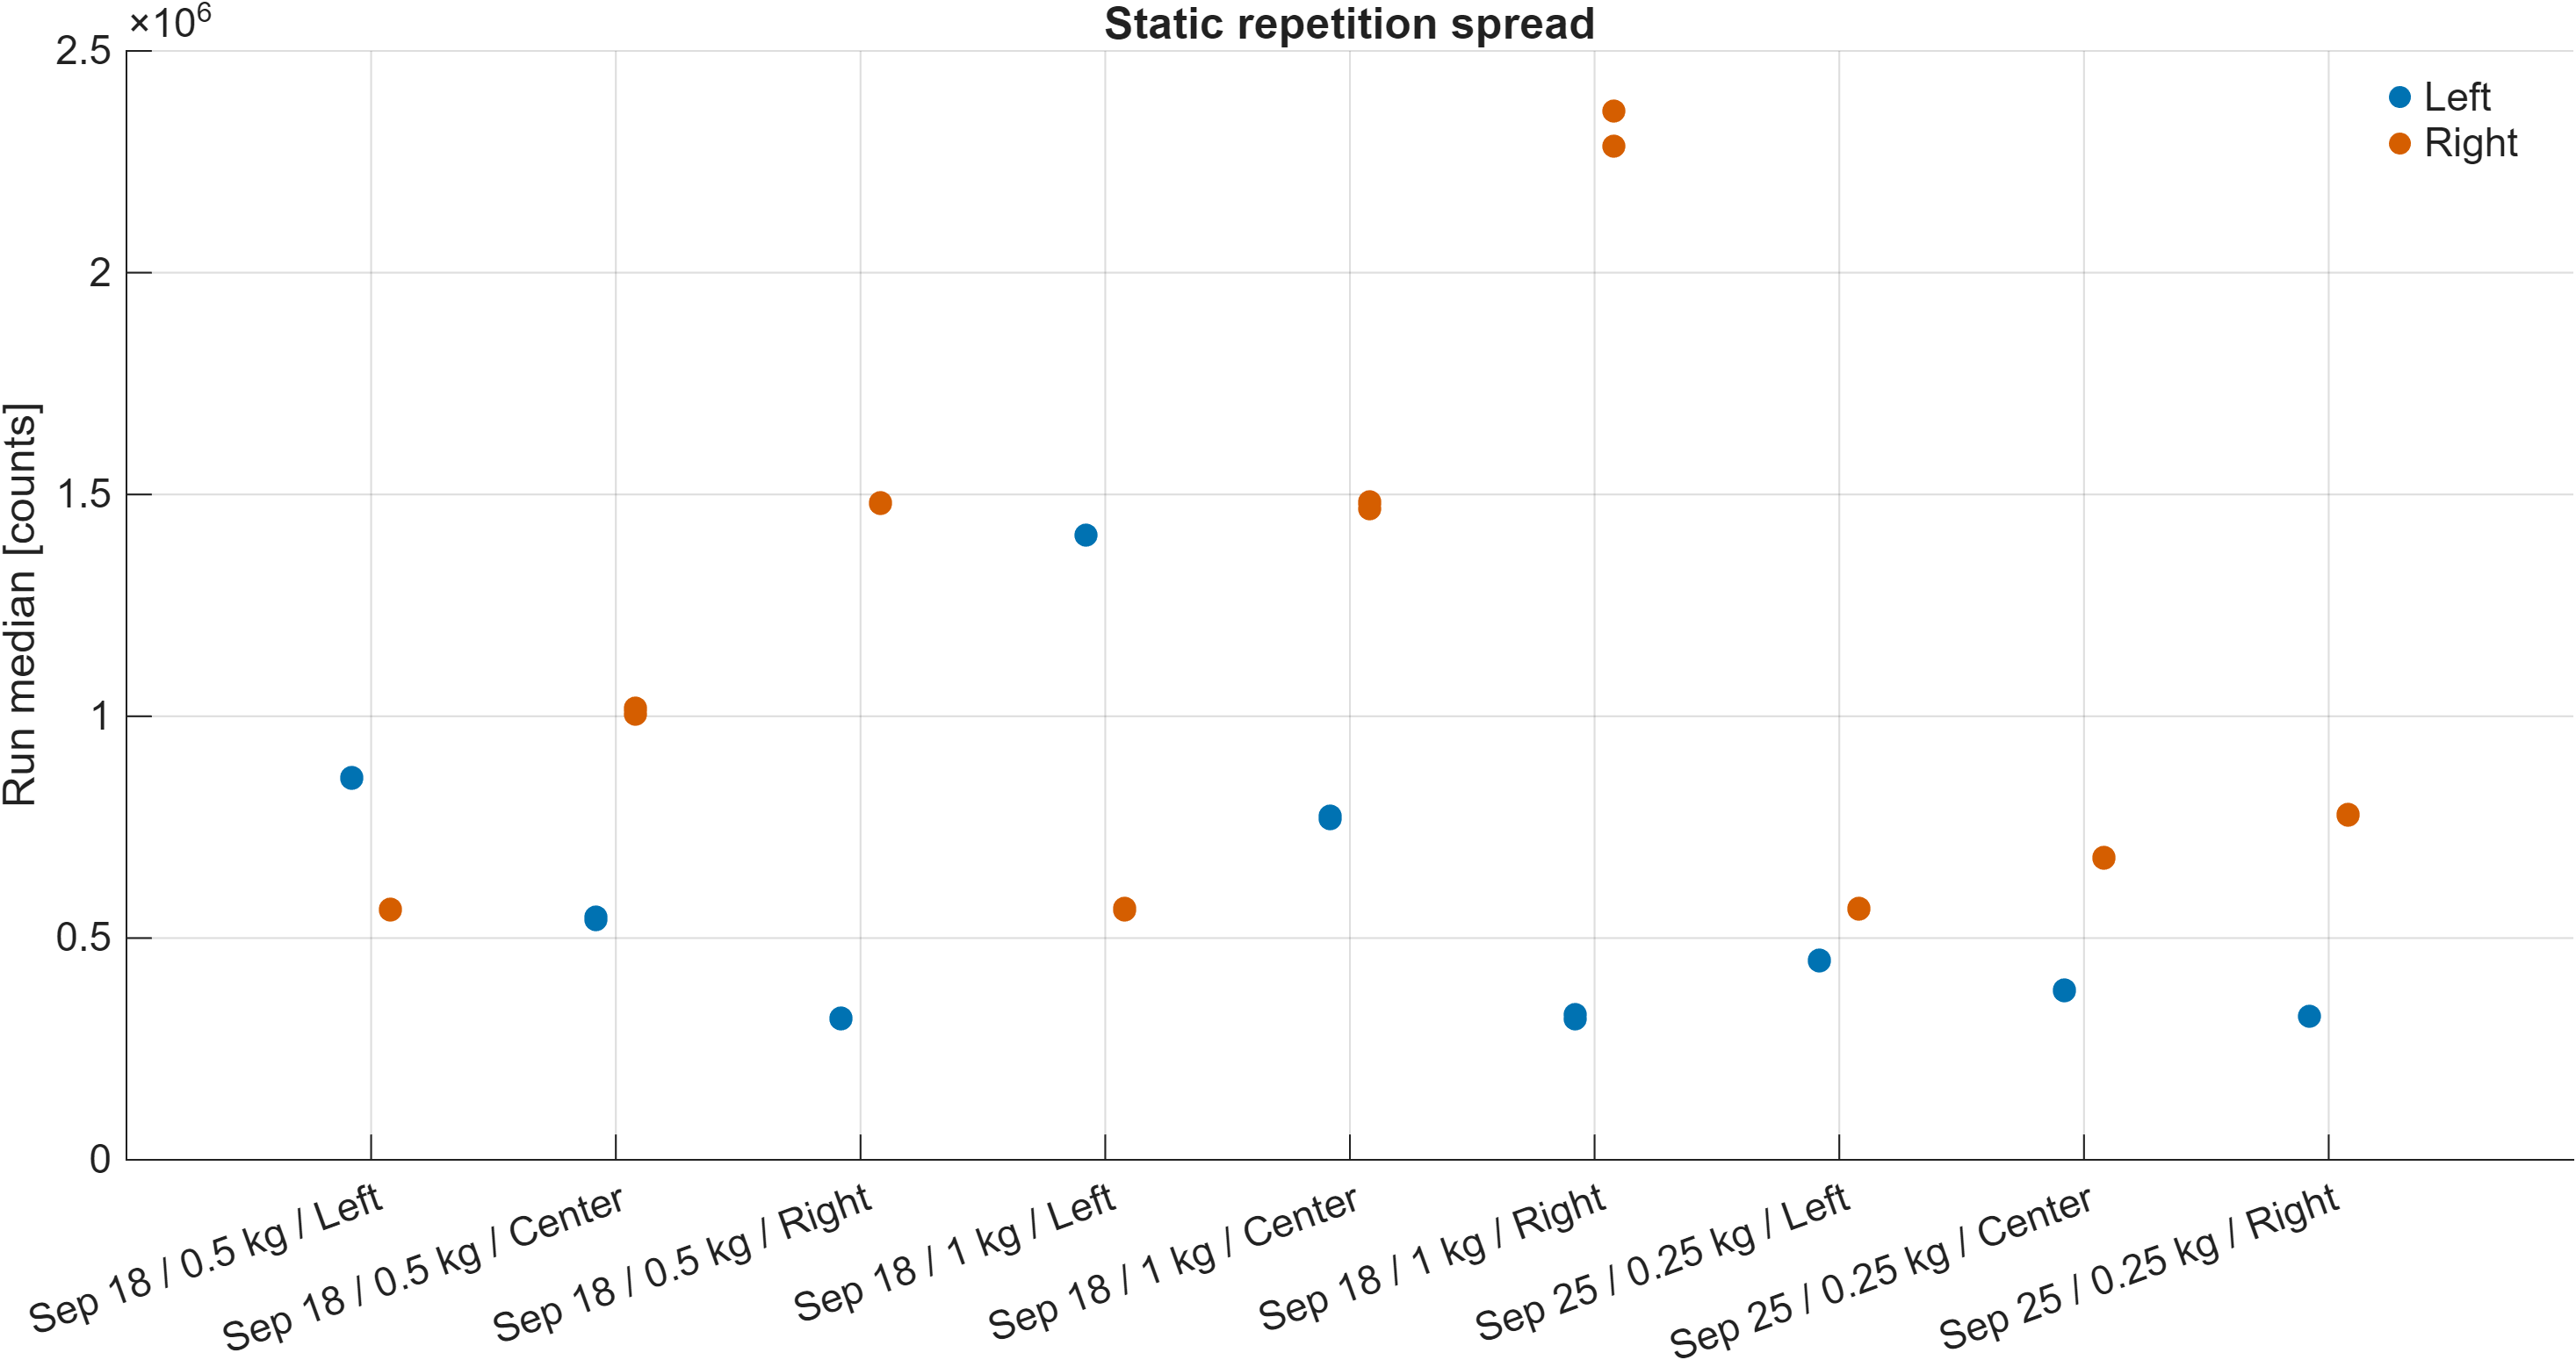
\includegraphics[width=\textwidth,height=0.37\textheight,keepaspectratio]{figures/F08_static_repeatability.png}
\caption{Individual run medians within equivalent static conditions.}\label{fig:F08}
\end{figure}
The September 18 run medians are relatively reproducible compared with their absolute count levels: between-run coefficients of variation range from 0.015 to 1.932 percent. The largest value belongs to the right channel at 1 kg/right loading, where the standard deviation is 45176 counts, substantially larger than the 1076-count standard deviation at 0.5 kg/right loading. This localized loss of repeatability deserves a mounting and acquisition check before fitting position sensitivity. These percentages describe raw medians, whose large offsets can make relative scatter appear small. Stable medians also suppress isolated excursions visible in time histories. No acceptance tolerance or calibration uncertainty was specified, so the data support descriptive repeatability, not a declaration that measurement performance is acceptable.\par

\Needspace{5\baselineskip}
\section{Load Position Sensitivity}
The position comparisons retain mass and batch strata. Left, center and right refer to metadata position labels. The normalized raw-signal contribution is included to describe relative channel output, but differing offsets and gains prevent identifying it with a support reaction or load fraction.

\renewcommand{\thefigure}{F09}
\begin{figure}[H]\centering
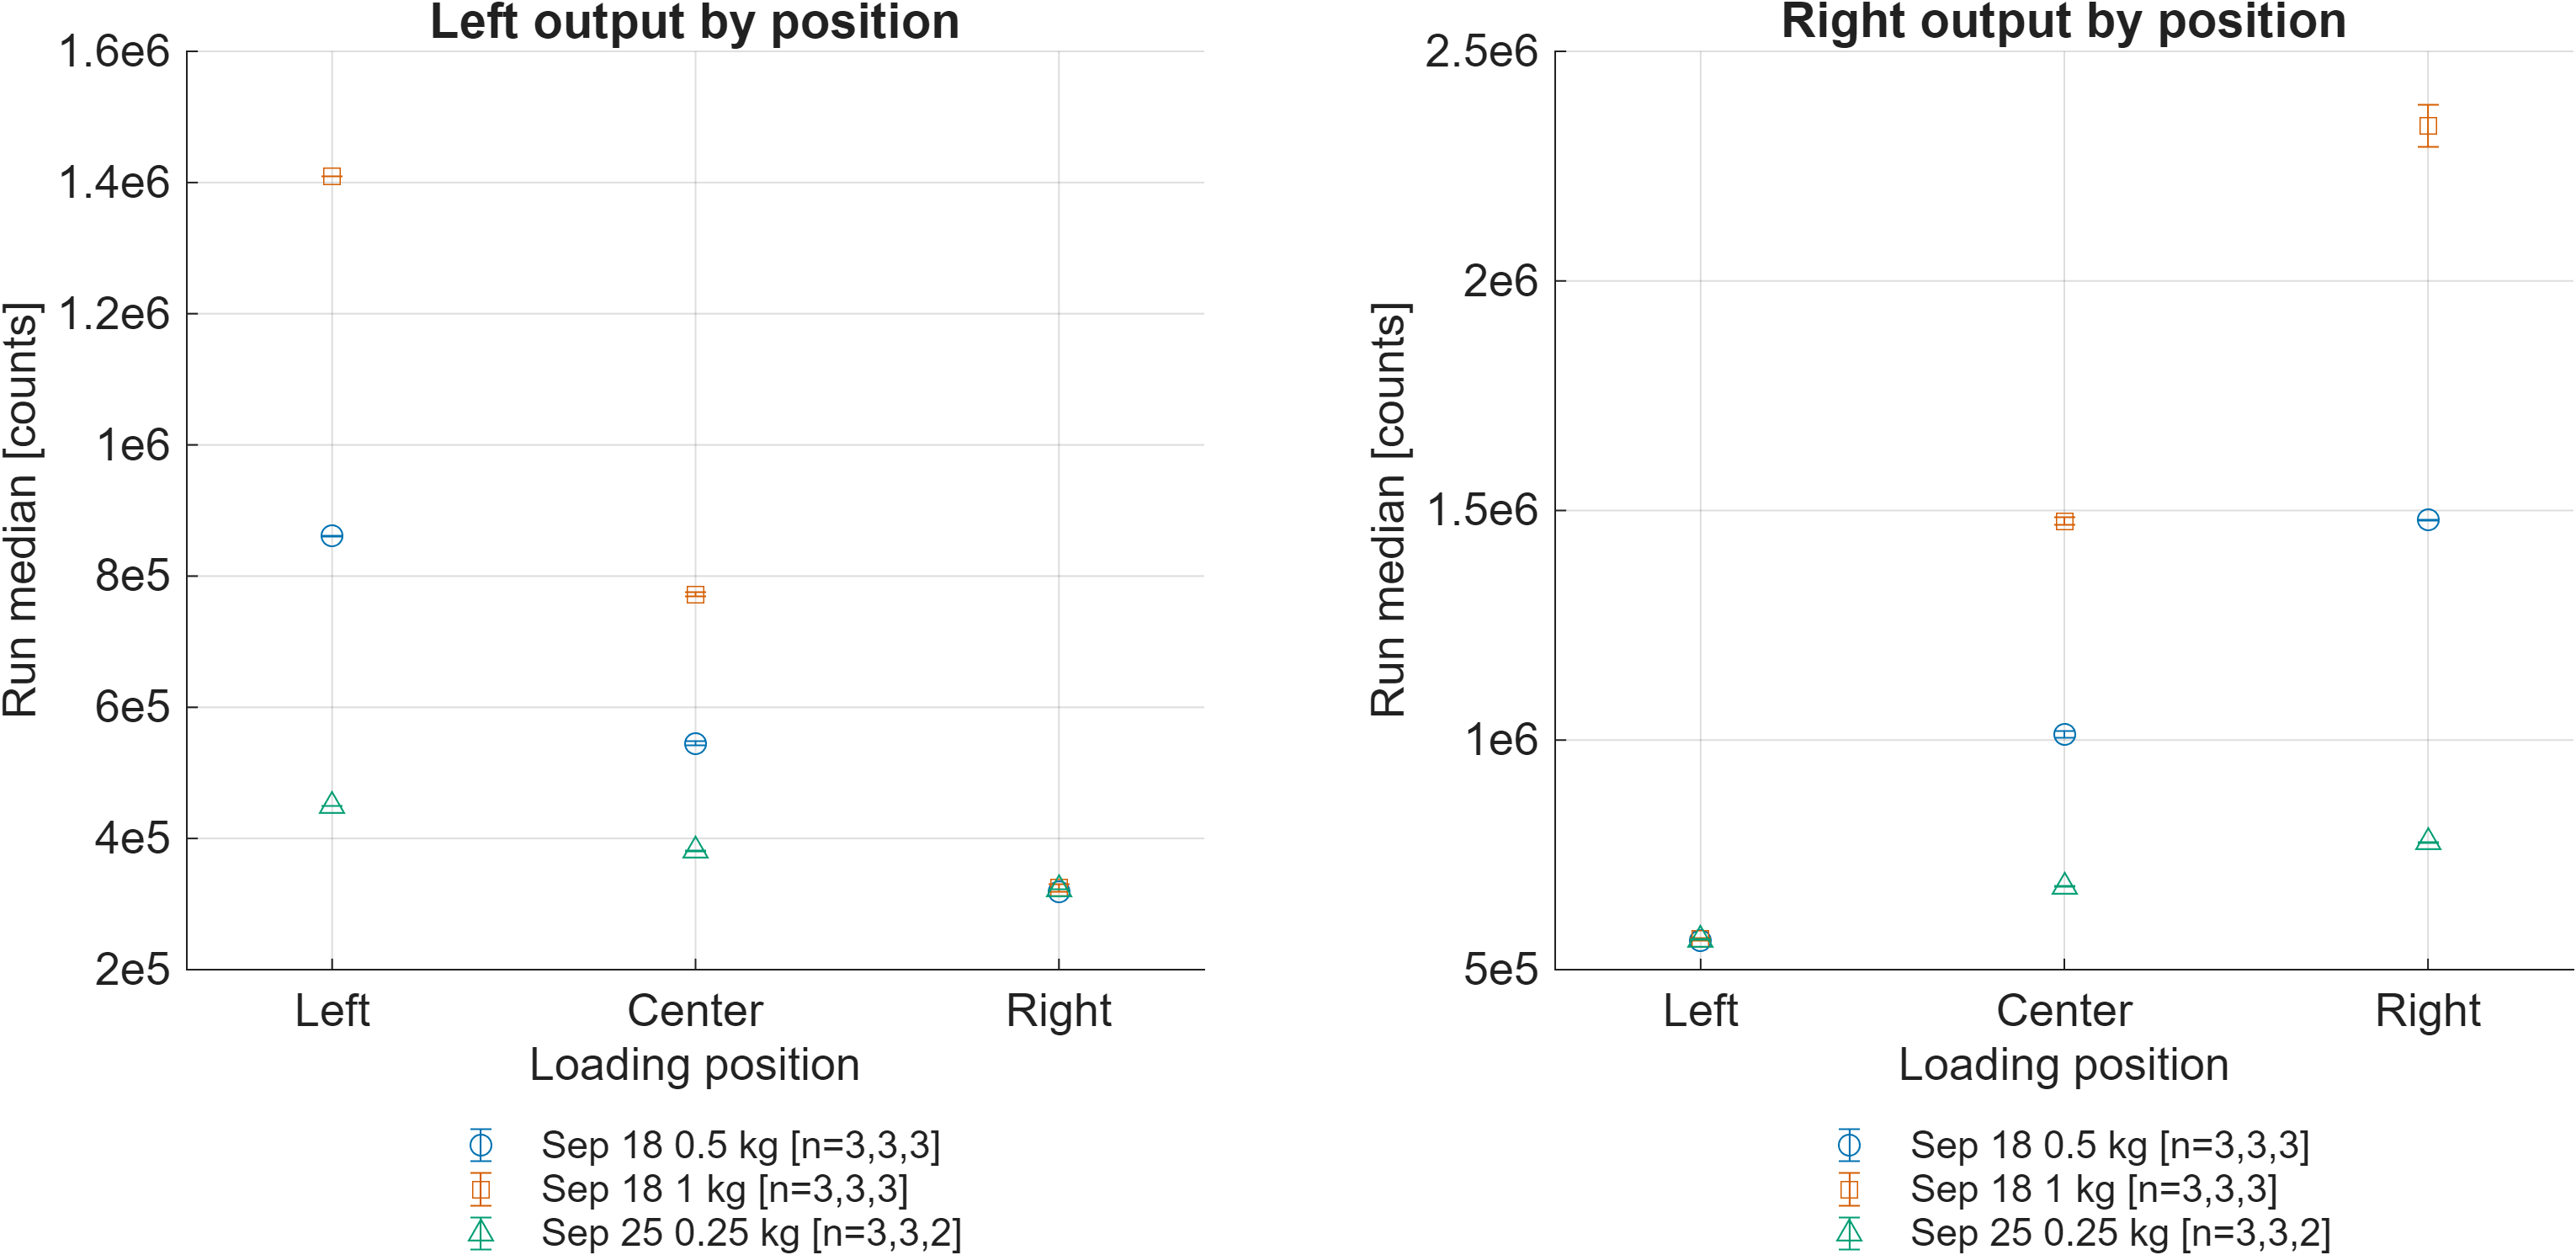
\includegraphics[width=\textwidth,height=0.37\textheight,keepaspectratio]{figures/F09_position_response.png}
\caption{Left, center and right loading positions at matched mass and batch.}\label{fig:F09}
\end{figure}
Moving a 1 kg load from left to right decreases the left-channel mean of run medians from 1409088 to 324512 counts (77.0 percent), while increasing the right channel from 566025 to 2337938 counts (313.0 percent). The center measurements lie between the endpoints. The same opposite ordering occurs at 0.5 kg in September 18 and at 0.25 kg in September 25, making position sensitivity more consistent than an across-batch mass calibration. Redistribution of the load path is a plausible mechanism, although sensor mounting and channel gains contribute to the observed scale. Because these are raw counts with unknown tare, the relative changes cannot be interpreted as support-reaction percentages. Independent position trials would be needed to test prediction accuracy.\par

\renewcommand{\thefigure}{F10}
\begin{figure}[H]\centering
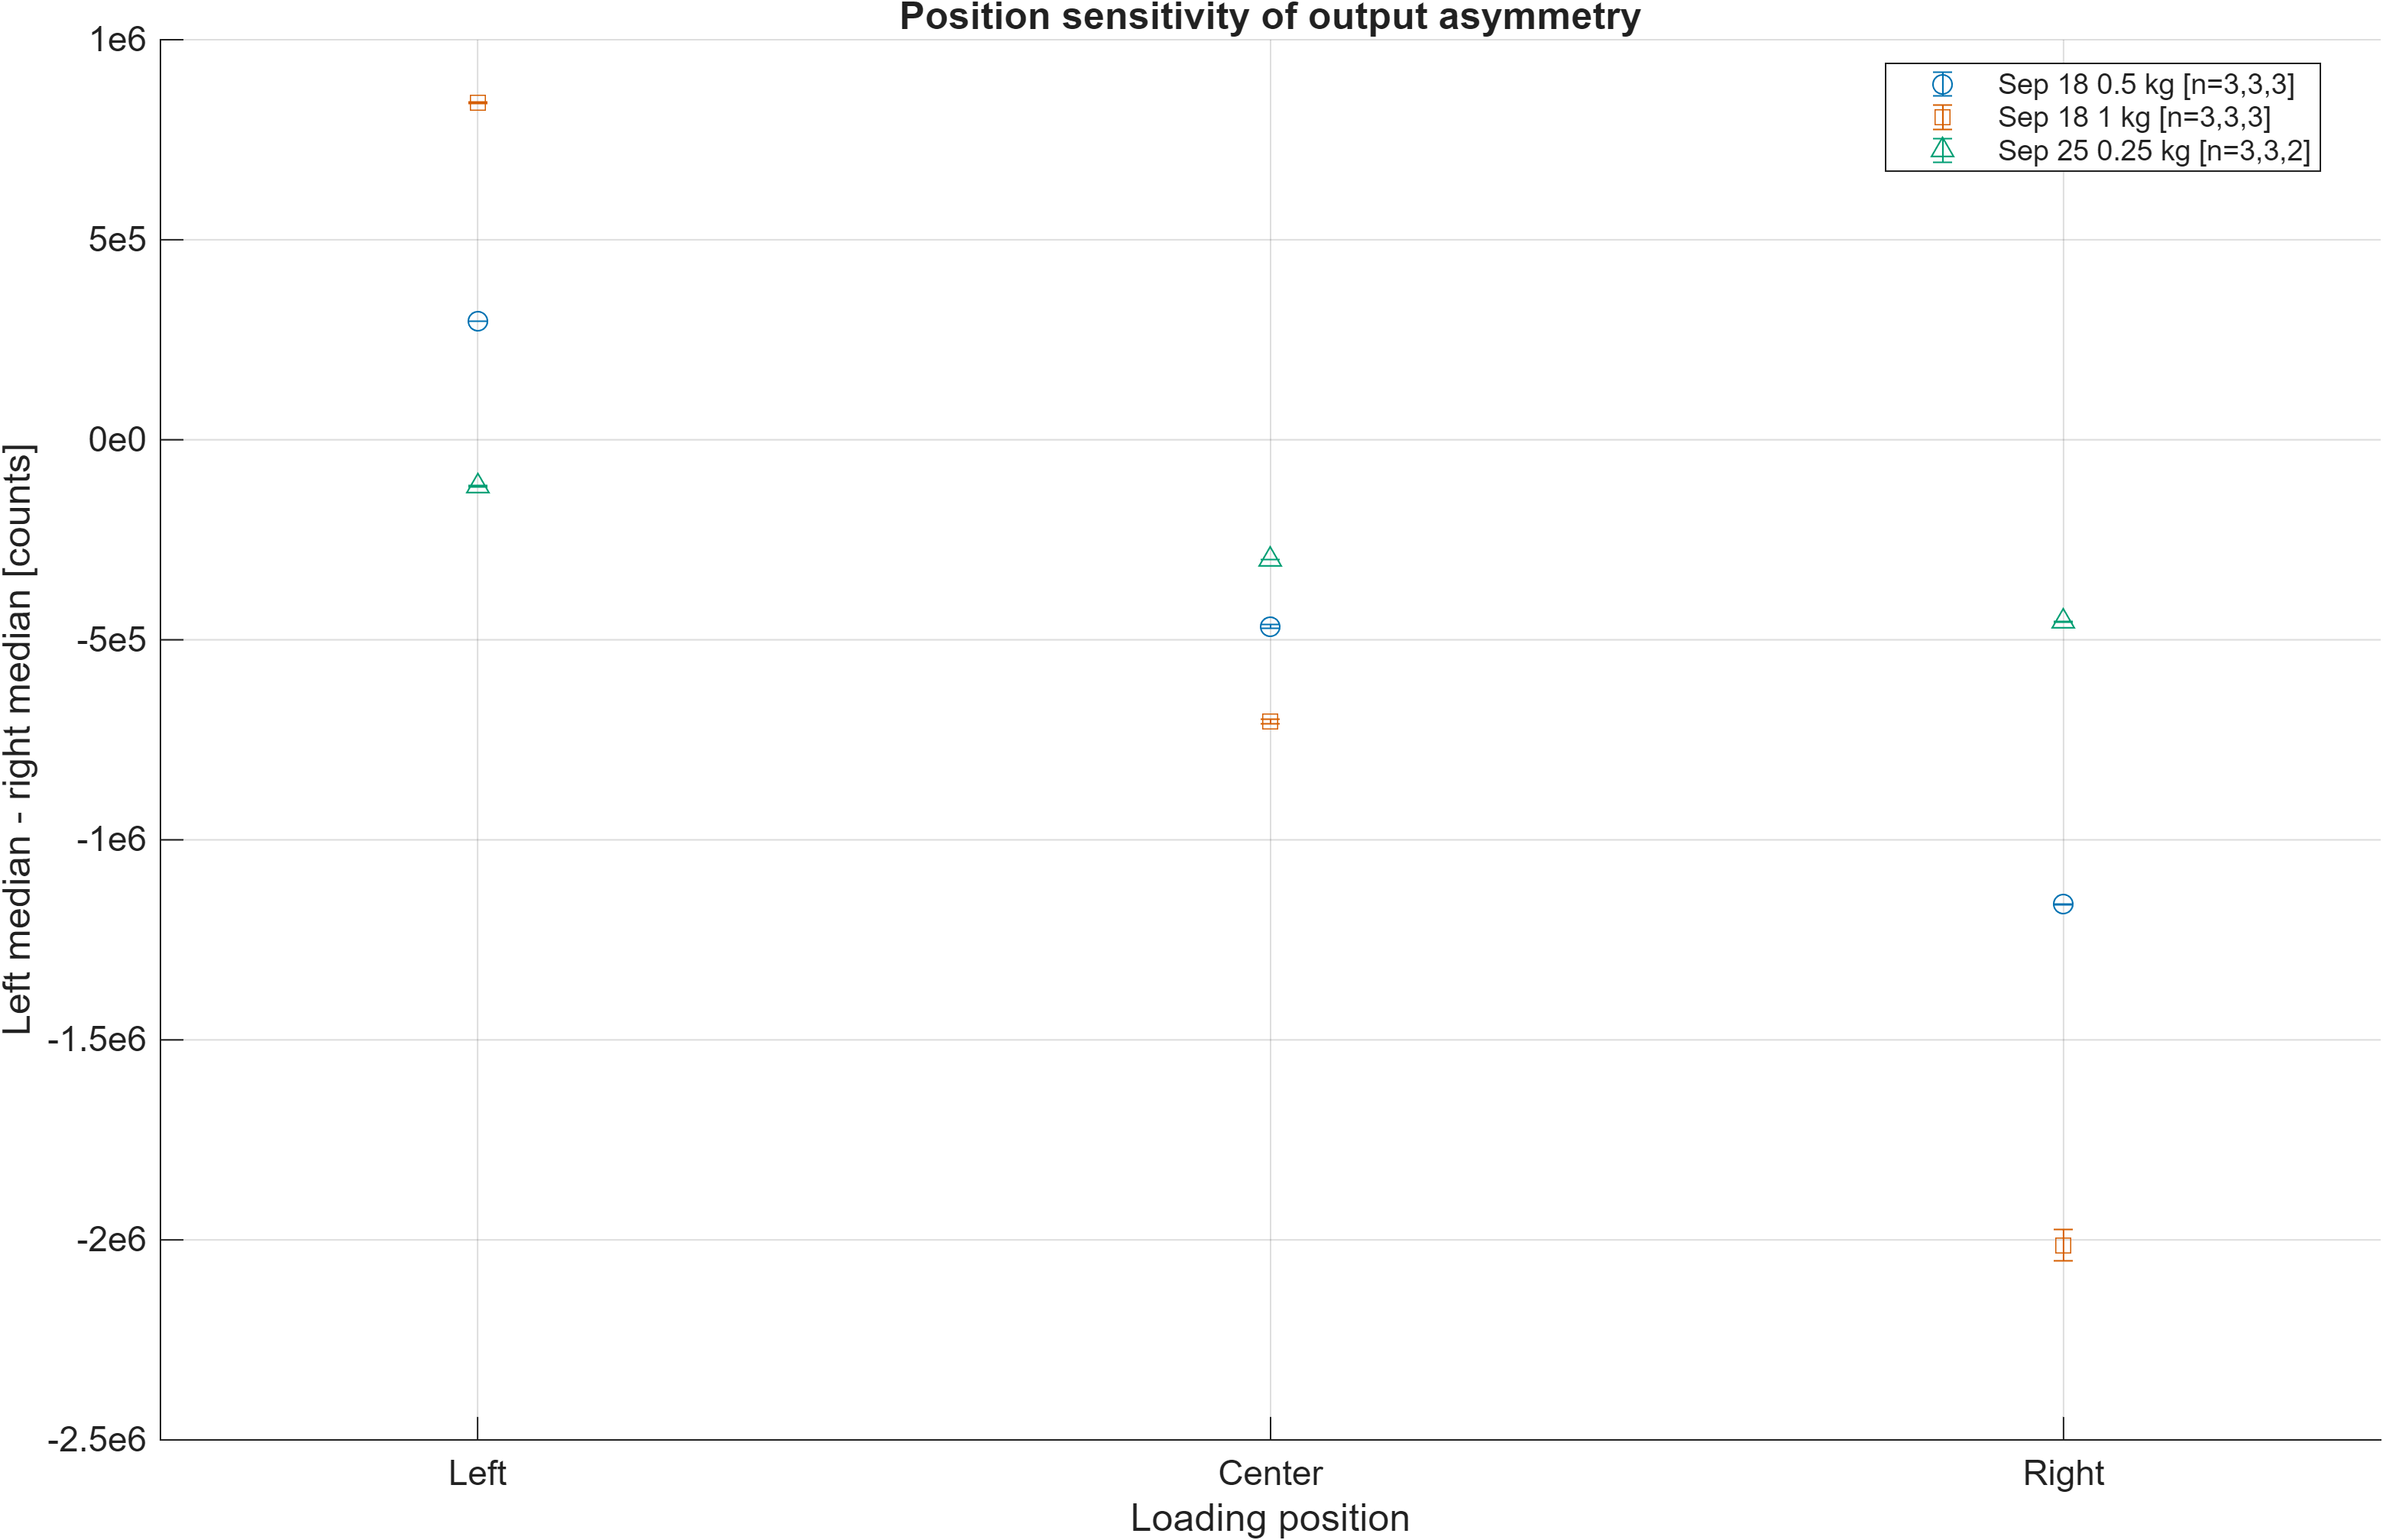
\includegraphics[width=\textwidth,height=0.37\textheight,keepaspectratio]{figures/F10_position_asymmetry.png}
\caption{Position-dependent raw output asymmetry within mass and batch strata.}\label{fig:F10}
\end{figure}
Asymmetry falls consistently as the load moves right within each mass/batch stratum. At 1 kg the group means are 843062, -704453 and -2013427 counts for left, center and right, respectively. This ordered separation is potentially useful for identifying load location from a pair of sensors. It also reveals why the channel difference must not be interpreted as a force balance: the center result is far from zero, and all three September 25 0.25 kg positions have negative differences. Channel offsets or unequal gains can shift the entire relation without destroying its ordering. The trend is encouraging for a calibrated measurement model, but repetition scatter, acquisition artifacts and limited independent positions prevent claiming validated localization.\par

\renewcommand{\thefigure}{F11}
\begin{figure}[H]\centering
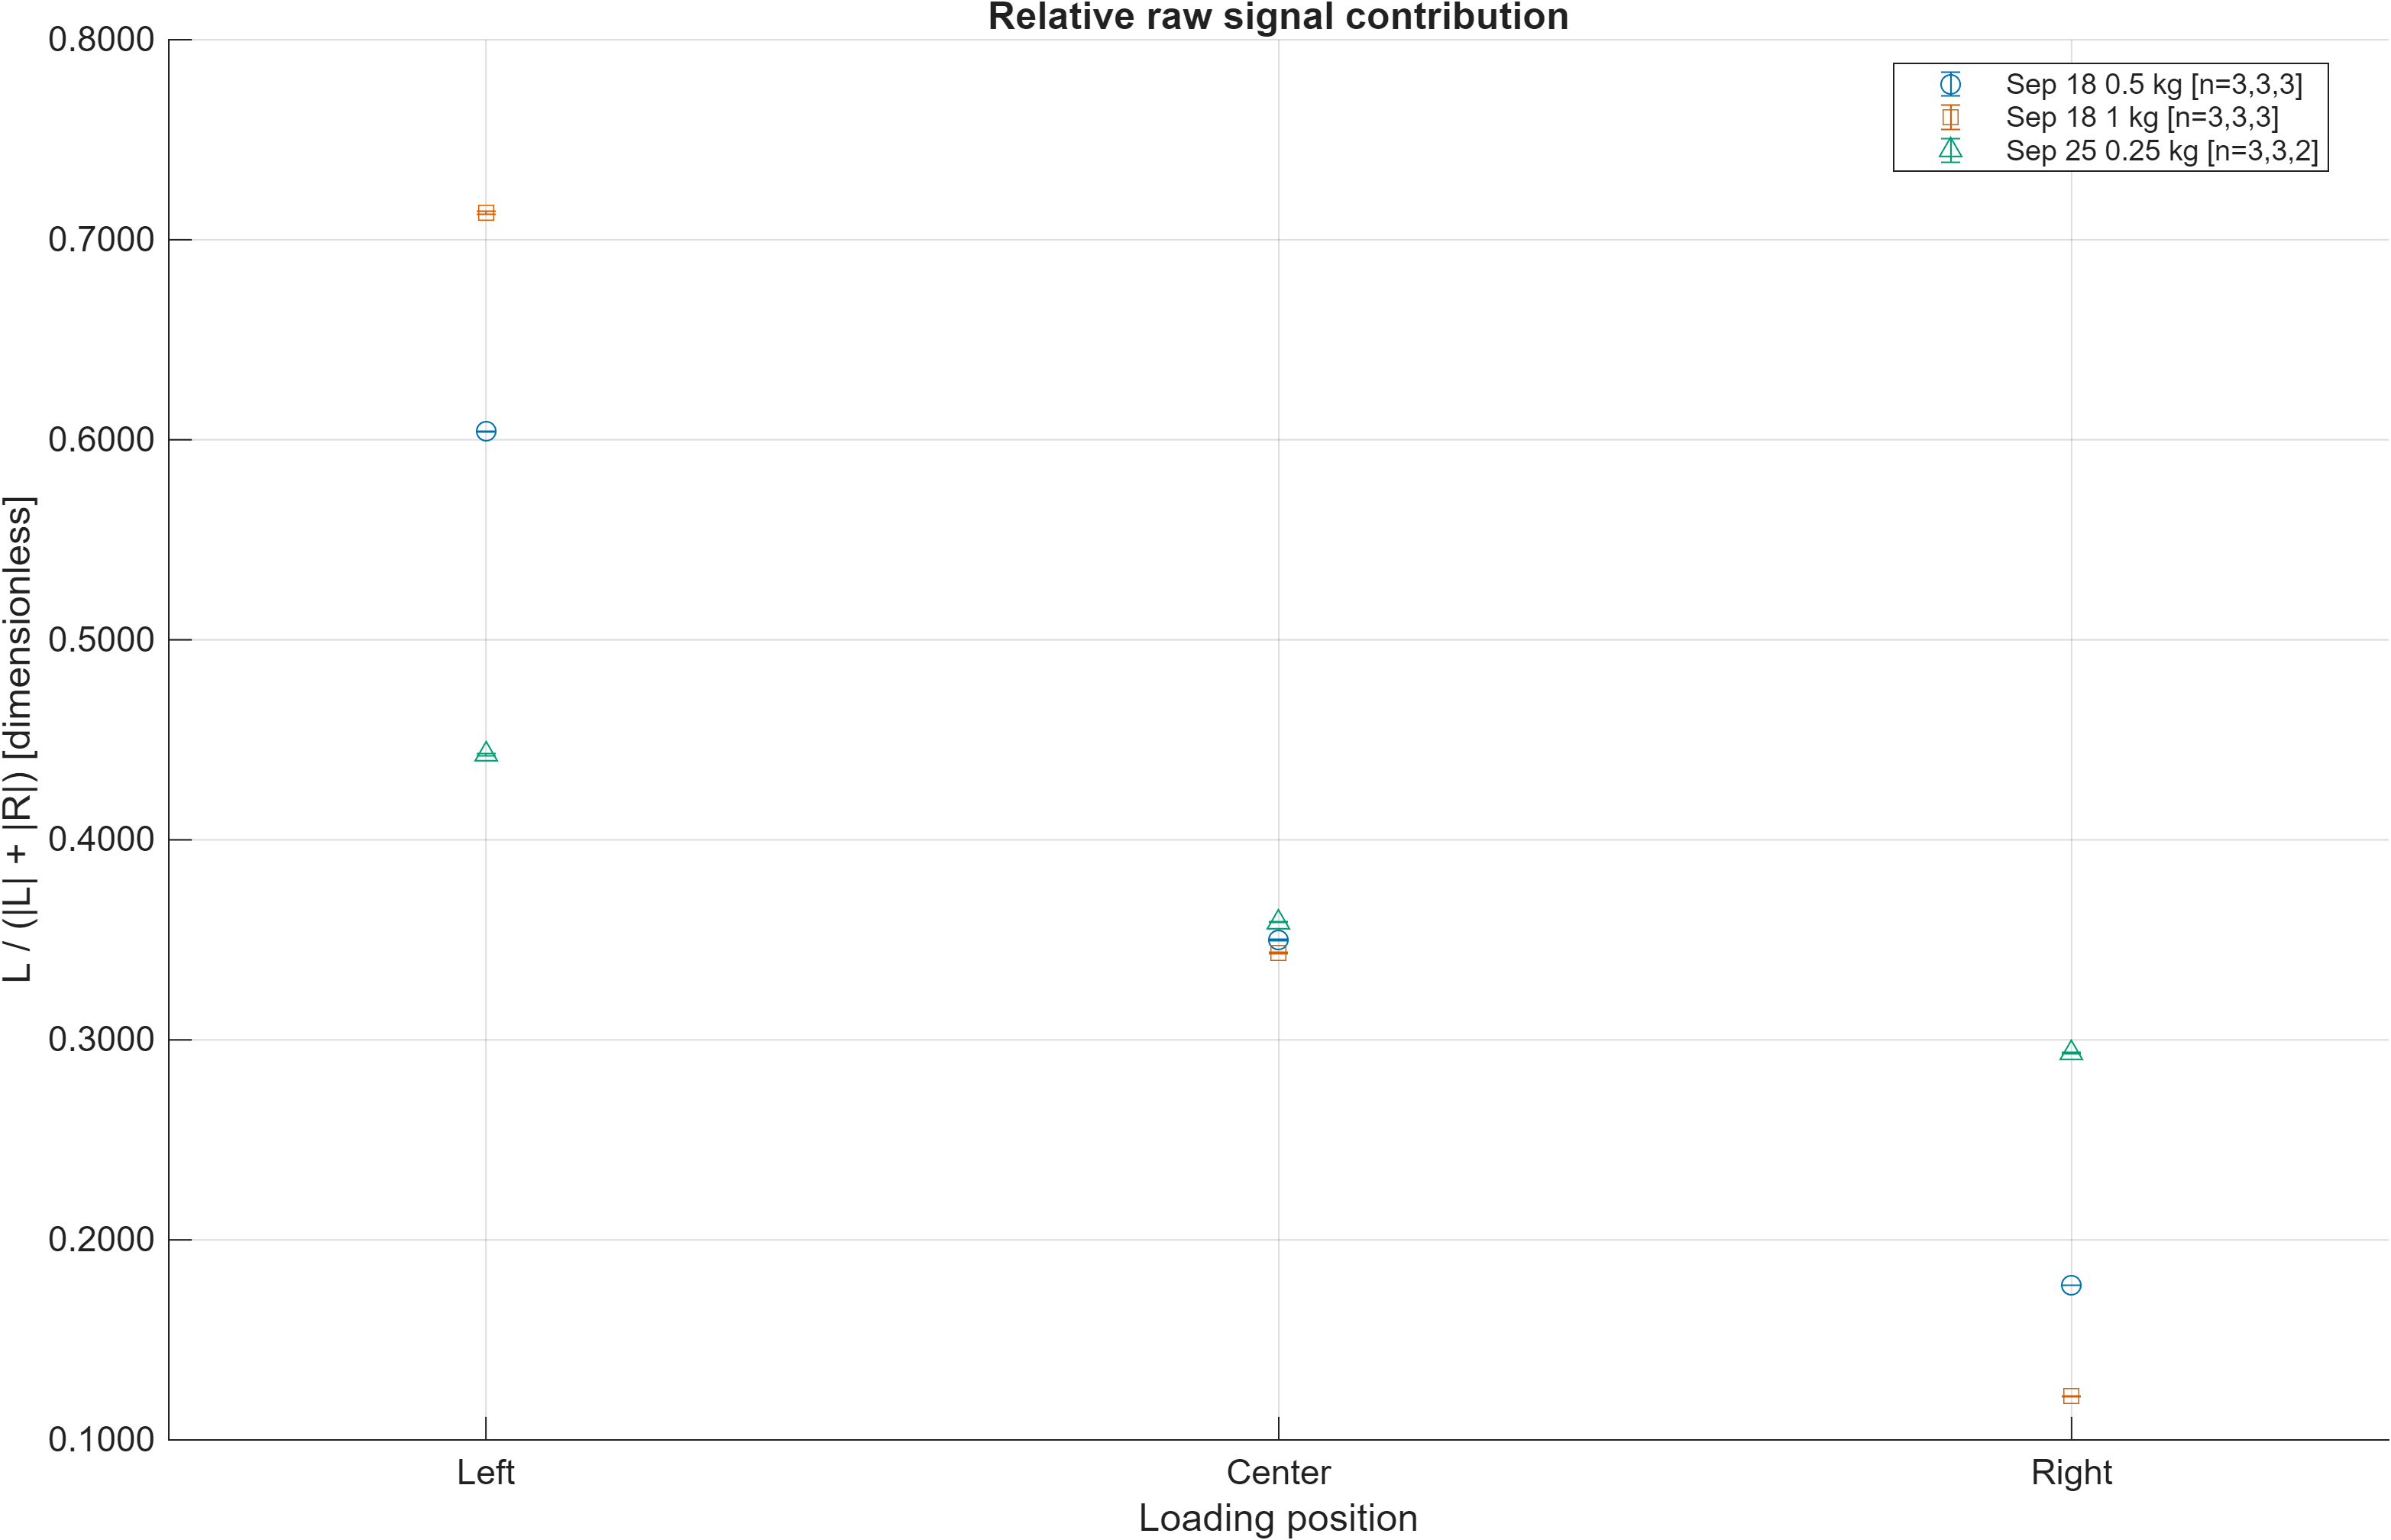
\includegraphics[width=\textwidth,height=0.37\textheight,keepaspectratio]{figures/F11_relative_signal_distribution.png}
\caption{Normalized left raw-output contribution by load position.}\label{fig:F11}
\end{figure}
For the 1 kg series, the normalized left raw-signal contribution decreases from 0.713 at left loading to 0.343 at center and 0.122 at right. The corresponding 0.5 kg endpoints are 0.604 and 0.177. The consistent direction compresses the two-channel position pattern into a bounded descriptor, but the center ratio is not 0.5 and the relation shifts with mass. These deviations are expected to be sensitive to nonzero sensor offsets and unequal gains, not just mechanics. The ratio may be useful as an empirical feature after calibration and controlled validation, but it is not a physical load-sharing fraction. Using it directly as a support reaction would discard the very offset and sensitivity information that these measurements show is important.\par

\Needspace{5\baselineskip}
\section{Vibration Response}
The unloaded September 18 vibration series provides a within-batch PWM comparison. Both cleaned acceleration levels and dynamic residuals are displayed. RMS and peak quantities apply to the existing cleaned signals. Earlier cleaning used a spike filter and interpolation of short missing runs, so original physical peaks may no longer be available.

\renewcommand{\thefigure}{F12}
\begin{figure}[H]\centering
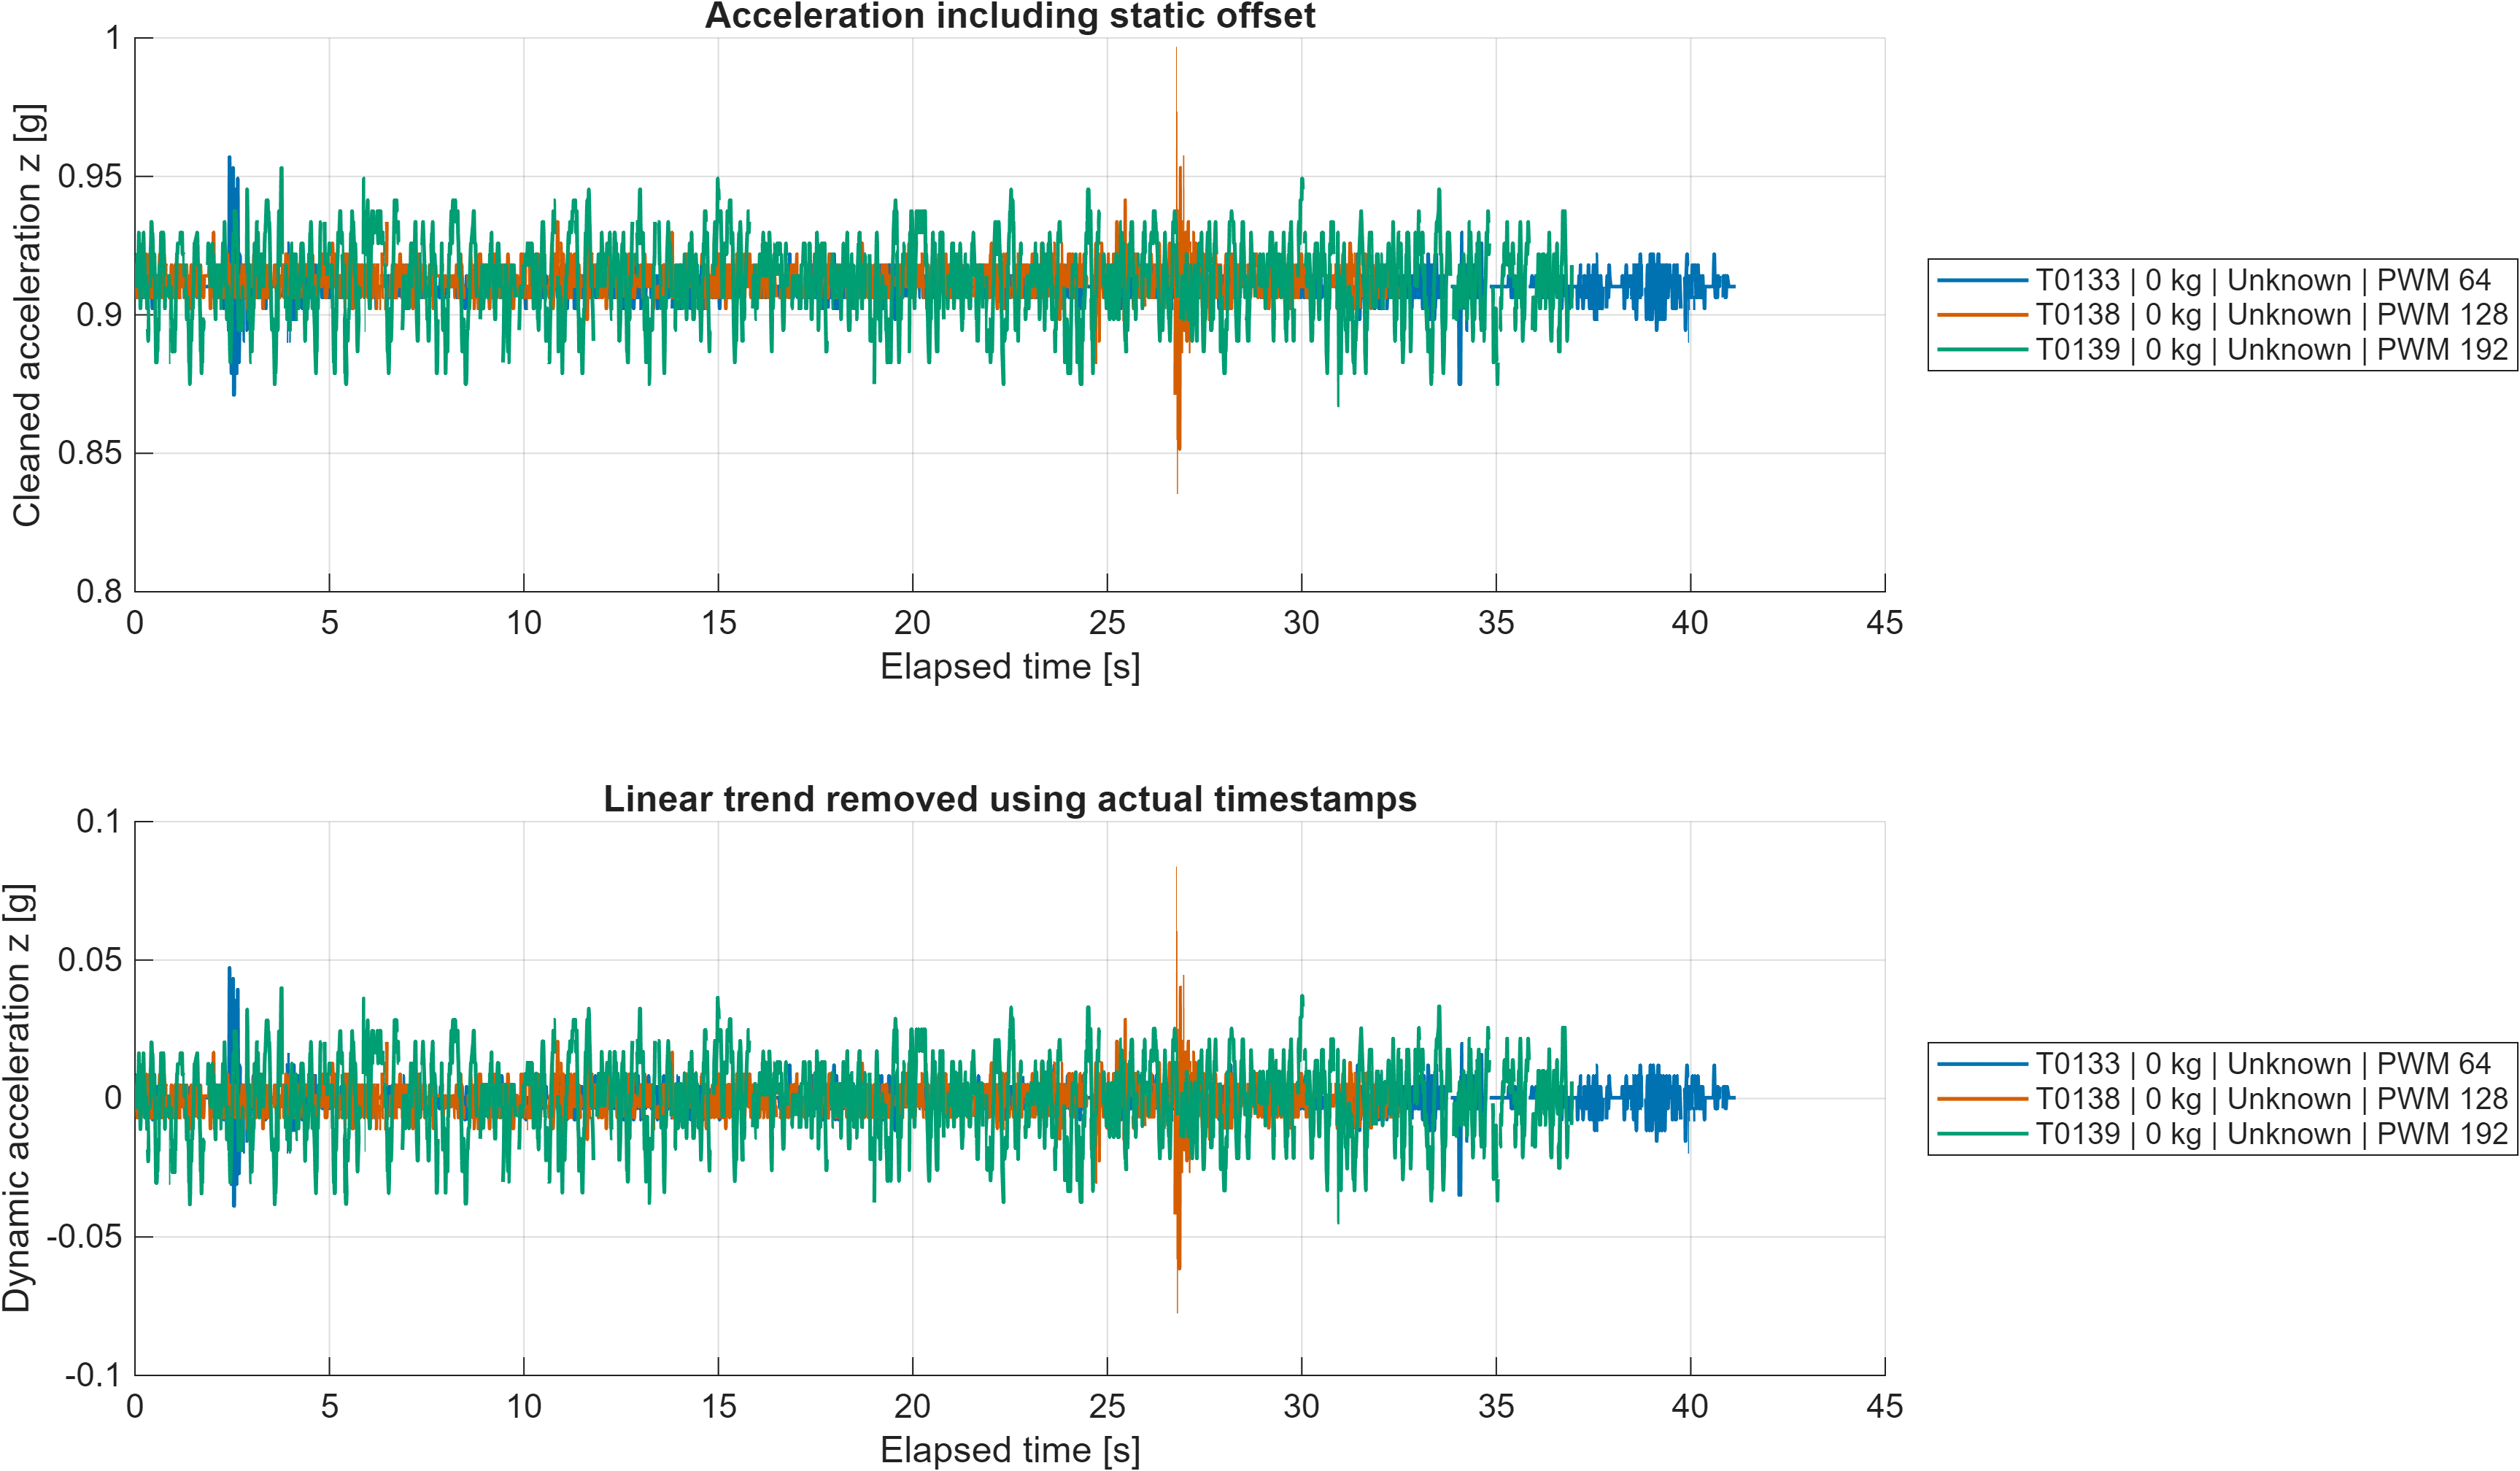
\includegraphics[width=\textwidth,height=0.37\textheight,keepaspectratio]{figures/F12_vibration_time_histories.png}
\caption{Cleaned and linearly detrended acceleration in representative no-load vibration runs.}\label{fig:F12}
\end{figure}
The selected waveforms separate a largely steady acceleration offset from much smaller dynamic fluctuations. Their detrended z RMS values are 0.00420, 0.00612 and 0.01440 g at PWM 64, 128 and 192. The highest command produces sustained broader fluctuations, whereas the PWM 128 representative includes a short, conspicuous excursion near the latter part of the record. This difference illustrates why RMS and maximum amplitude need not rank commands identically: a brief transient can dominate the peak without dominating the energy averaged over the recording. Increased forcing is plausible at higher command, but PWM does not identify excitation force or frequency. These are median-RMS representatives, not synchronized trials, and earlier cleaning may have altered individual spikes.\par

\renewcommand{\thefigure}{F13}
\begin{figure}[H]\centering
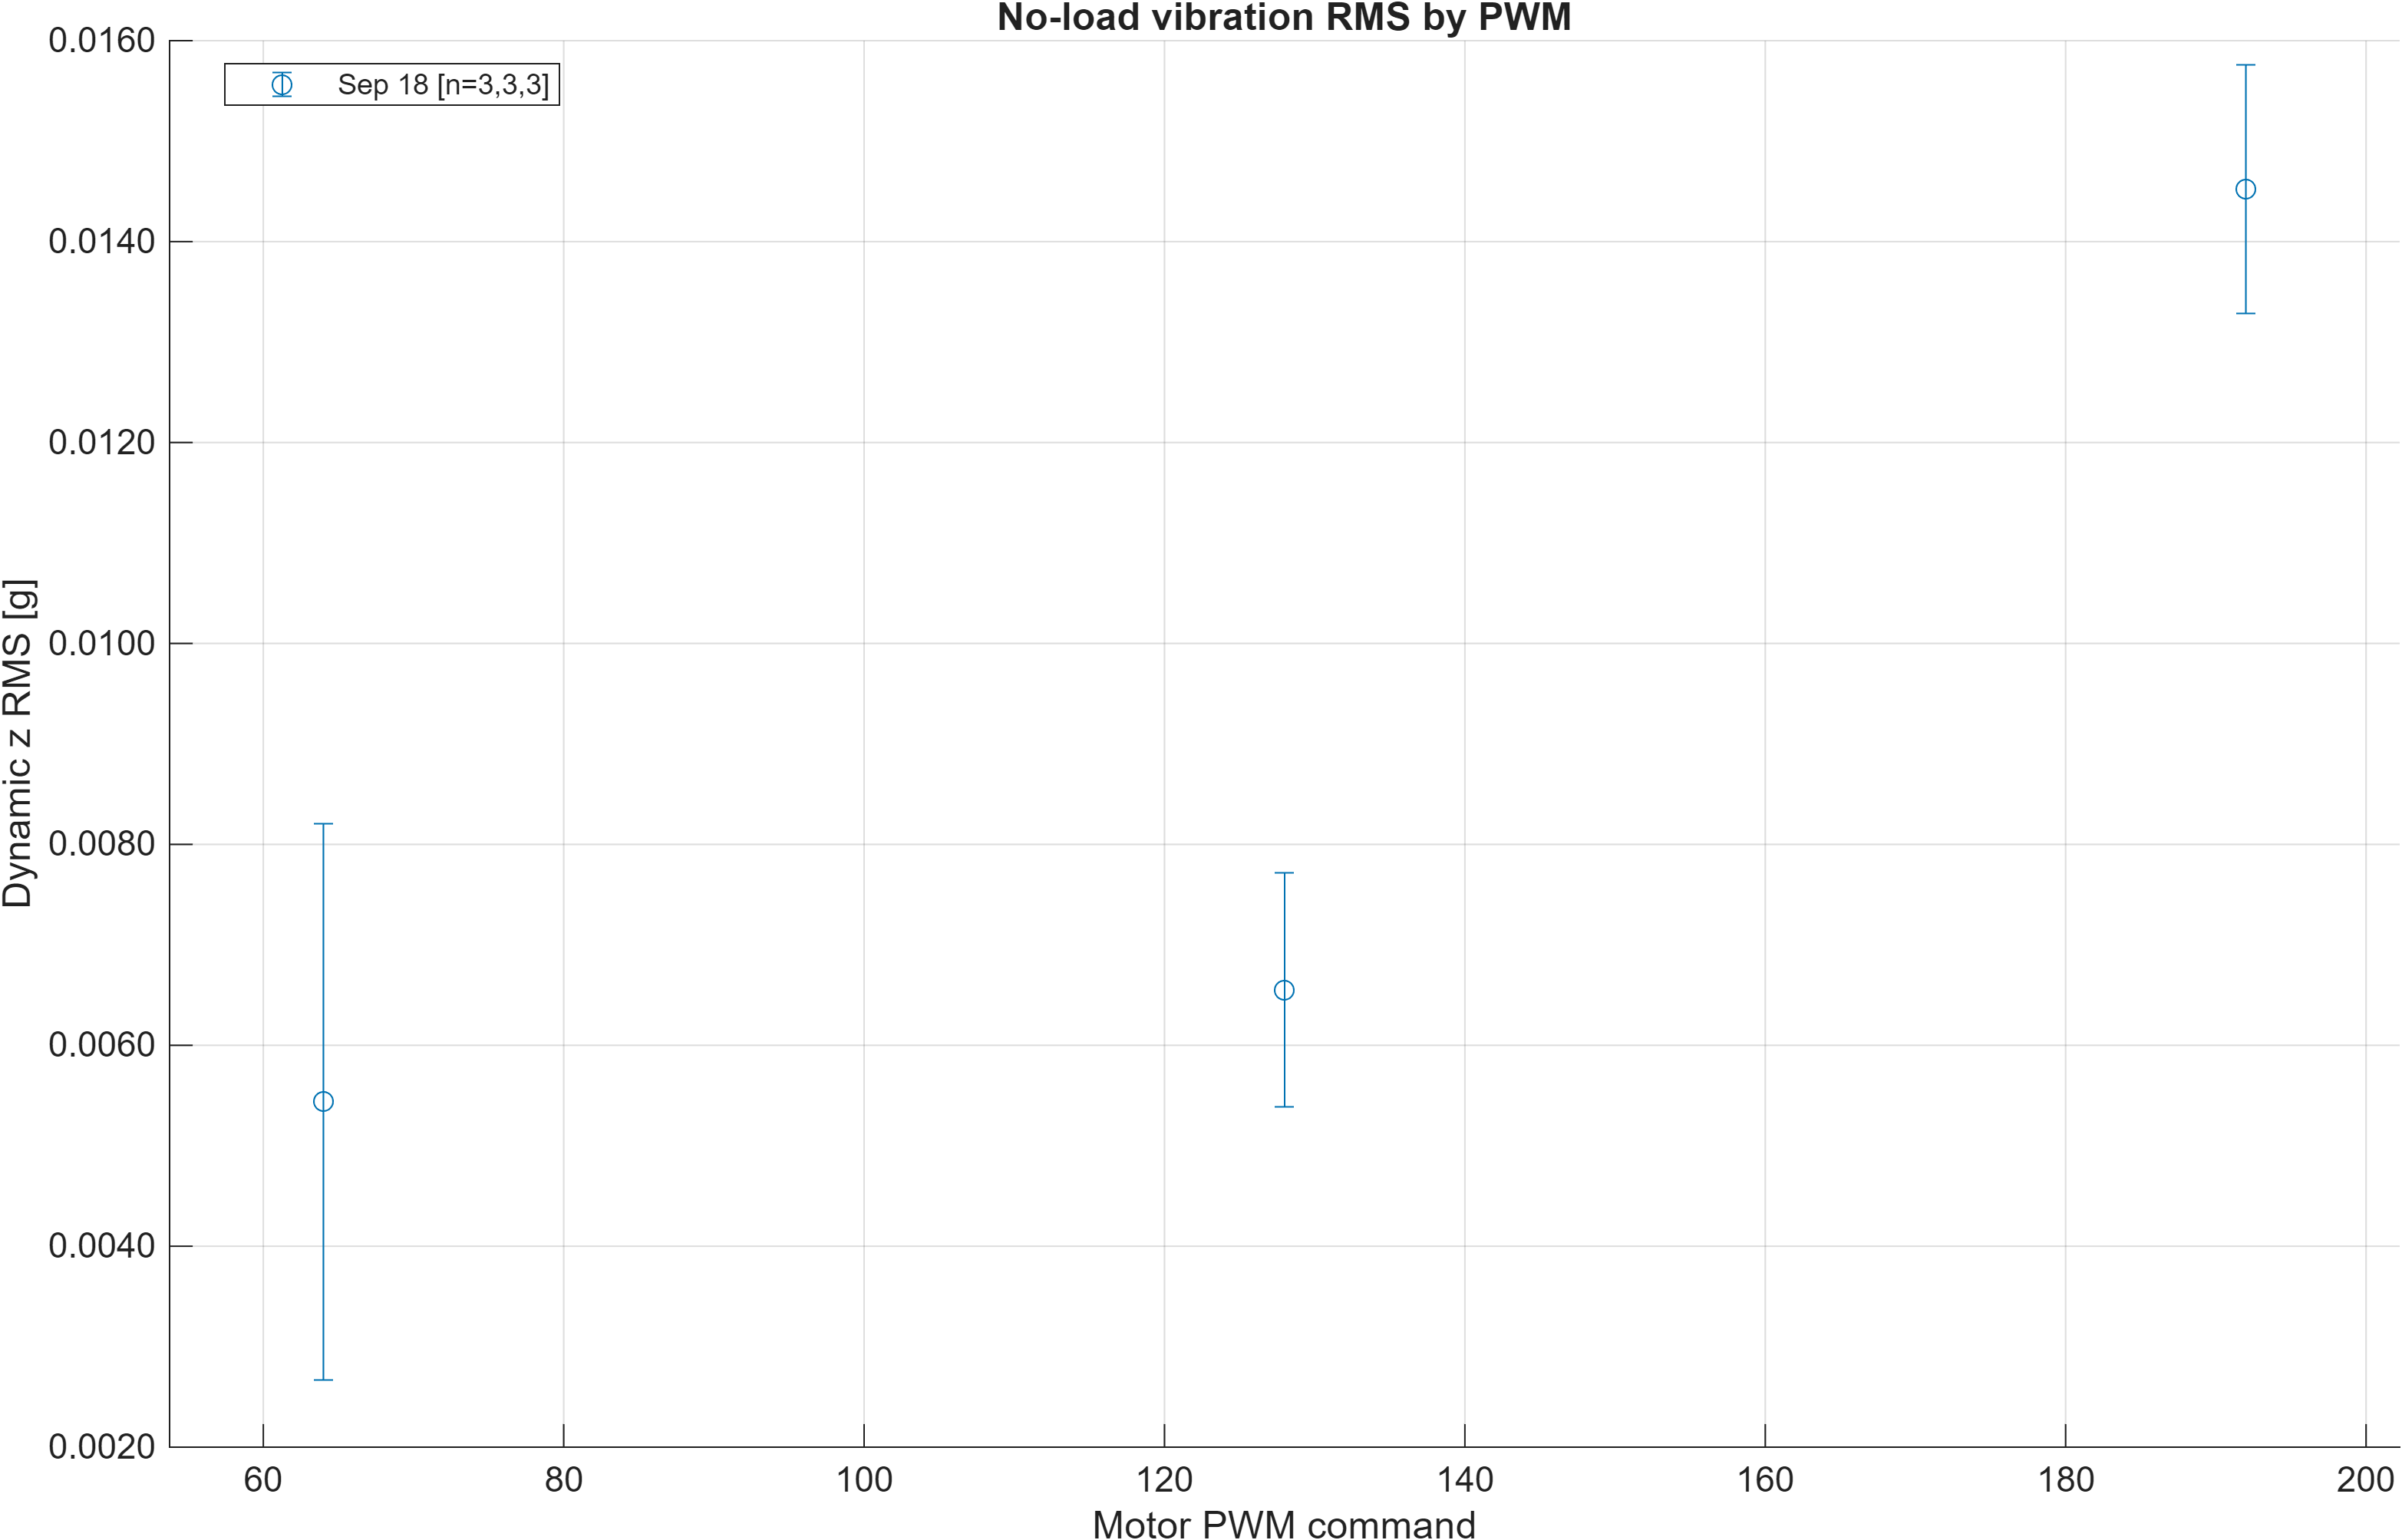
\includegraphics[width=\textwidth,height=0.37\textheight,keepaspectratio]{figures/F13_vibration_rms.png}
\caption{Dynamic acceleration RMS across the no-load PWM series.}\label{fig:F13}
\end{figure}
Mean unloaded z RMS increases monotonically from 0.00544 g at PWM 64 to 0.00655 g at 128 and 0.01452 g at 192. The increases are 20.5 percent for 64-to-128 and 121.7 percent for 128-to-192; the highest command is 167.1 percent above the lowest. The first increase is smaller than the PWM 64 between-run standard deviation of 0.00277 g, so that step is weak evidence of a repeatable change. The high-command separation is more pronounced relative to the plotted repetition spread. Greater excitation is a plausible explanation, but motor force, speed and structural response are not independently measured. These three-repetition results characterize sensitivity under this acquisition setup, not a calibrated or statistically validated command-response law.\par

\renewcommand{\thefigure}{F14}
\begin{figure}[H]\centering
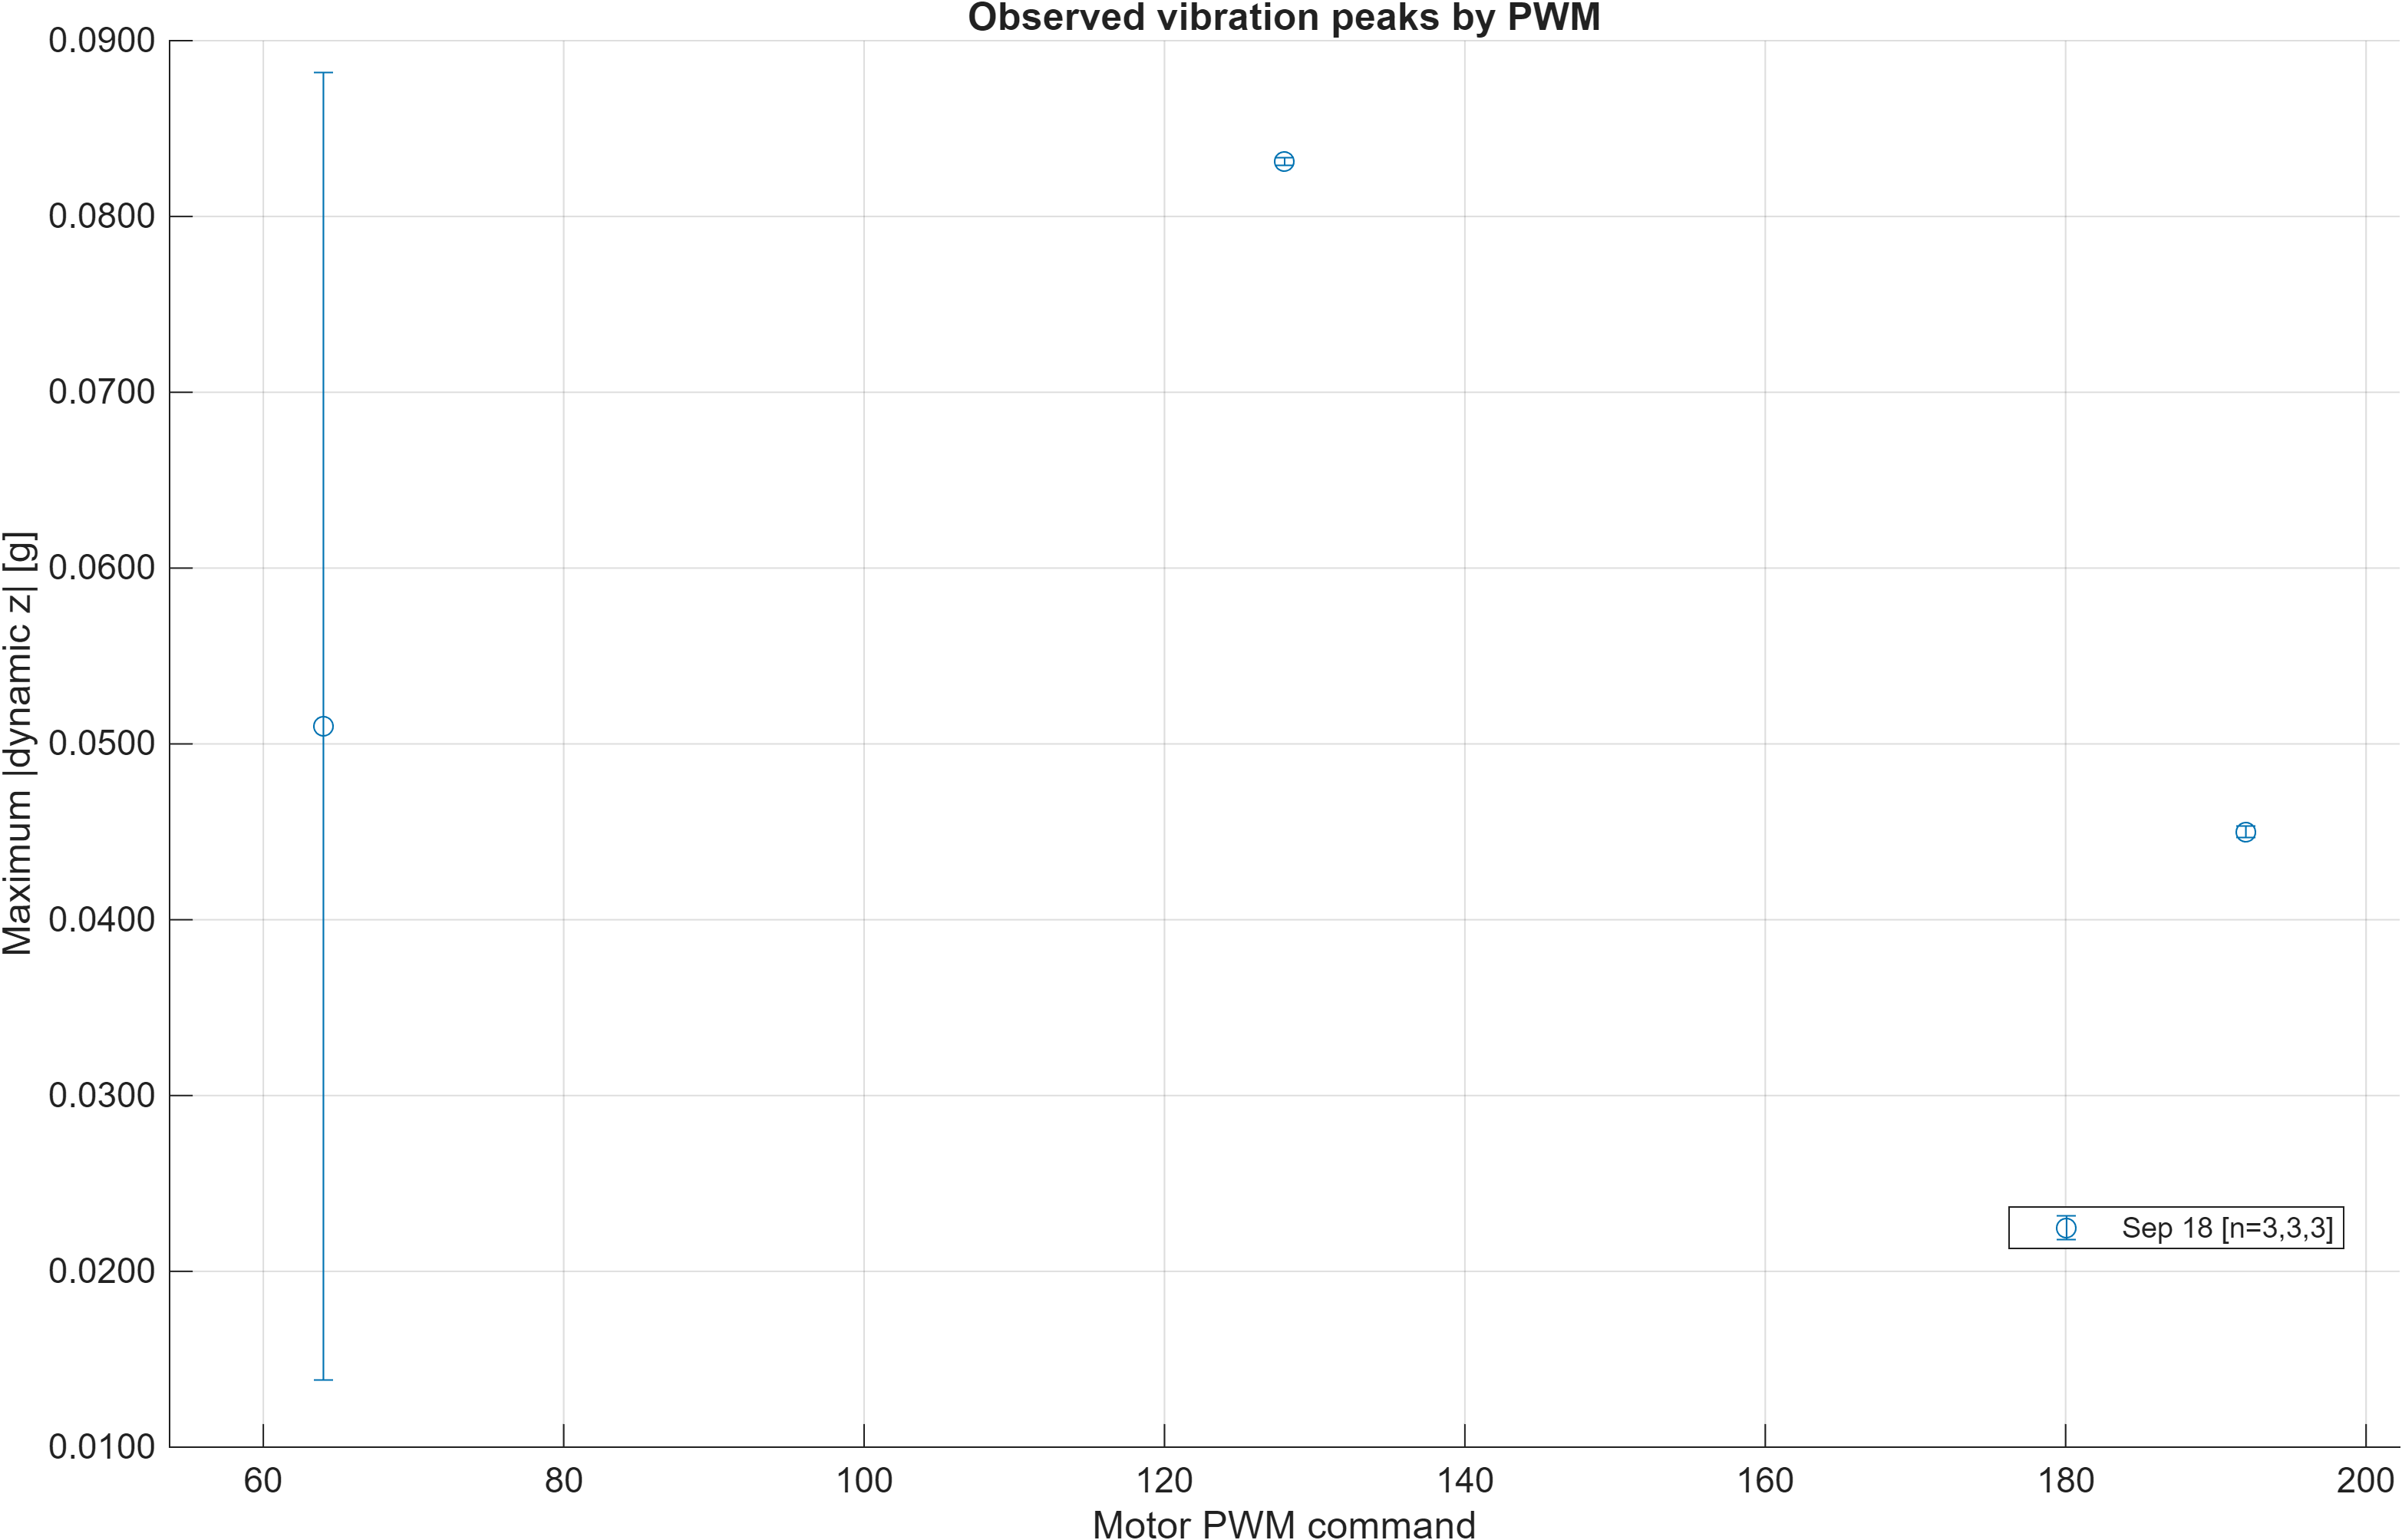
\includegraphics[width=\textwidth,height=0.37\textheight,keepaspectratio]{figures/F14_vibration_peaks.png}
\caption{Largest observed absolute detrended z acceleration in each no-load vibration run.}\label{fig:F14}
\end{figure}
Peak response is nonmonotonic: the mean observed maximum is 0.05102 g at PWM 64, 0.08313 g at 128 and 0.04499 g at 192. The last step decreases the peak by 45.9 percent even though RMS increases. This is a substantive counterexample to treating a higher motor command as a uniformly larger response. Short-lived excursions and differences in waveform concentration can reverse peak rankings while sustained fluctuations increase. PWM 64 peaks are especially variable, with a between-run standard deviation of 0.03718 g, compared with 0.00023 g at PWM 128. No extra smoothing was applied here, but upstream spike filtering remains a limitation. Peak-based alarm or model features therefore need event-level provenance and repeatability checks, rather than relying on command alone.\par

\renewcommand{\thefigure}{F15}
\begin{figure}[H]\centering
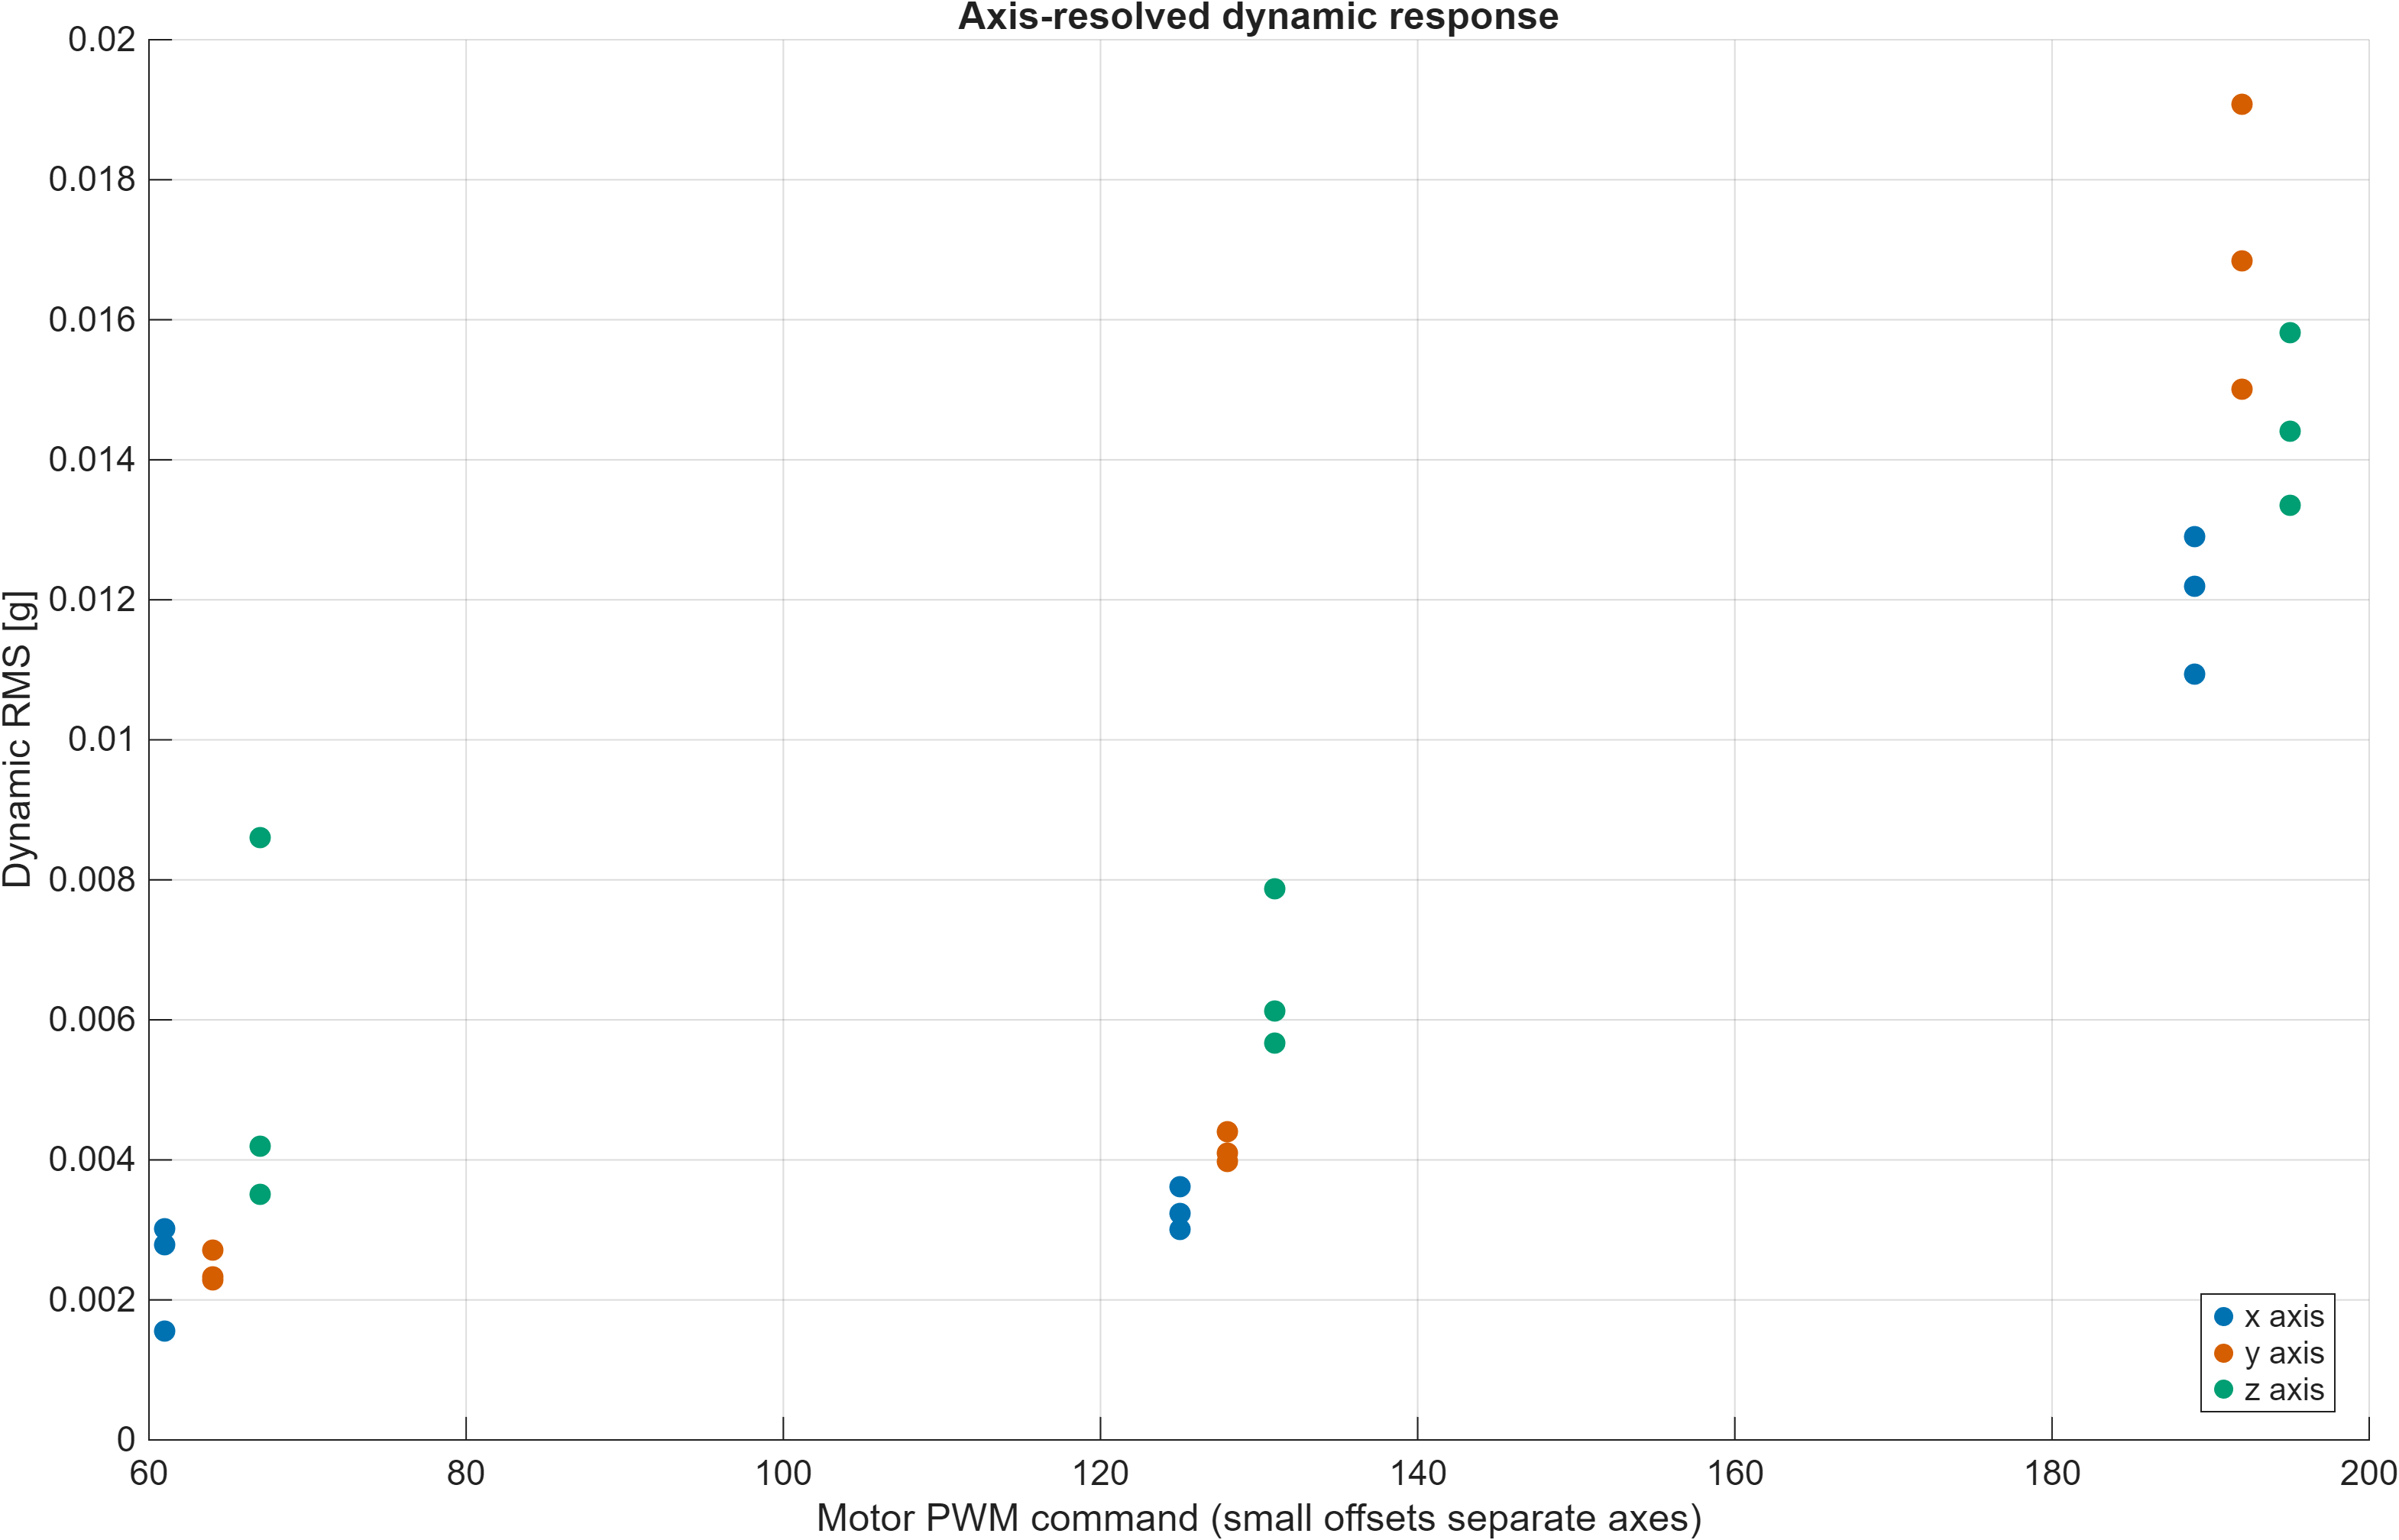
\includegraphics[width=\textwidth,height=0.37\textheight,keepaspectratio]{figures/F15_vibration_axes.png}
\caption{Axis-resolved RMS for the same no-load recordings.}\label{fig:F15}
\end{figure}
Dynamic response is not confined to the recorded z axis. At PWM 192, mean x/y/z RMS is 0.01201/0.01698/0.01452 g; y exceeds z by 16.9 percent. At PWM 64, z is 2.21 times x, so the dominant measured direction changes with command. From the lowest to highest PWM, x and y increase by factors 4.89 and 6.95, larger than the z factor 2.67. Direction-dependent excitation, sensor orientation and changes in structural motion could all contribute. The result argues for retaining all three axes in future system identification rather than reducing the measurement to z alone. It does not establish a mode shape: spatial measurements, orientation verification and excitation characterization are missing.\par

\Needspace{5\baselineskip}
\section{Frequency-Domain Analysis}
Timing is audited before spectral analysis. The cleaner converted milliseconds to seconds and had already removed nonincreasing timestamps or selected a reset segment. The present cleaned timestamps can therefore reveal remaining jitter and gaps but cannot reconstruct discarded raw resets. The recurring increments near 0.09--0.10 s, in otherwise approximately 0.01 s sampling, are treated conservatively as missing acquisition intervals. Their acquisition cause cannot be established from cleaned data alone.

For each run, the algorithm splits at missing acceleration, nonincreasing timestamps, or a timestamp increment greater than 1.5 times the median. It selects the longest remaining interval and requires at least four seconds, at least 256 samples, and maximum interval deviation no greater than 20 percent of the local median. Four seconds gives at least two cycles at the lowest inspected 0.5 Hz and a nominal Fourier spacing no coarser than 0.25 Hz. These are minimum engineering screening rules, not a certification of stationarity or anti-aliasing.

Only an accepted interval is linearly interpolated onto its median-increment grid, without extrapolation or bridging rejected gaps. Base MATLAB supplies linear detrending and fft. The periodic Hann window is evaluated directly as $w_n=0.5-0.5\cos(2\pi n/N)$. The amplitude is $|\mathrm{FFT}(w a_{dyn})|/\sum w$, with positive-frequency bins doubled except DC and, for even N, Nyquist. Frequencies are $k f_s/N$. The searched response-peak band is 0.5 Hz to the smaller of 40 Hz and 0.4 times the sampling rate. Bin spacing is not the ability to resolve neighboring tones: Hann windowing broadens spectral features. This is a response spectrum, not a transfer function because input force is not measured.

The MATLAB license test recognizes Signal Processing Toolbox entitlement, but hann, pwelch and spectrogram are not installed in this execution environment. This prevents the optional toolbox analyses, not the base-MATLAB FFT. Welch PSD and spectrograms are omitted.

1 recording passes the unchanged interval rules: T0236, from 13.106 to 20.505 s (7.399 s). Its 741 source samples become 740 grid values at 100.000 Hz, spanning 7.390 s, with FFT bin spacing 0.135135 Hz. The other 90 candidates fail continuity-duration screening. The first accepted spectrum is appended as F33 to preserve all existing figure identifiers.

\renewcommand{\thefigure}{F16}
\begin{figure}[H]\centering
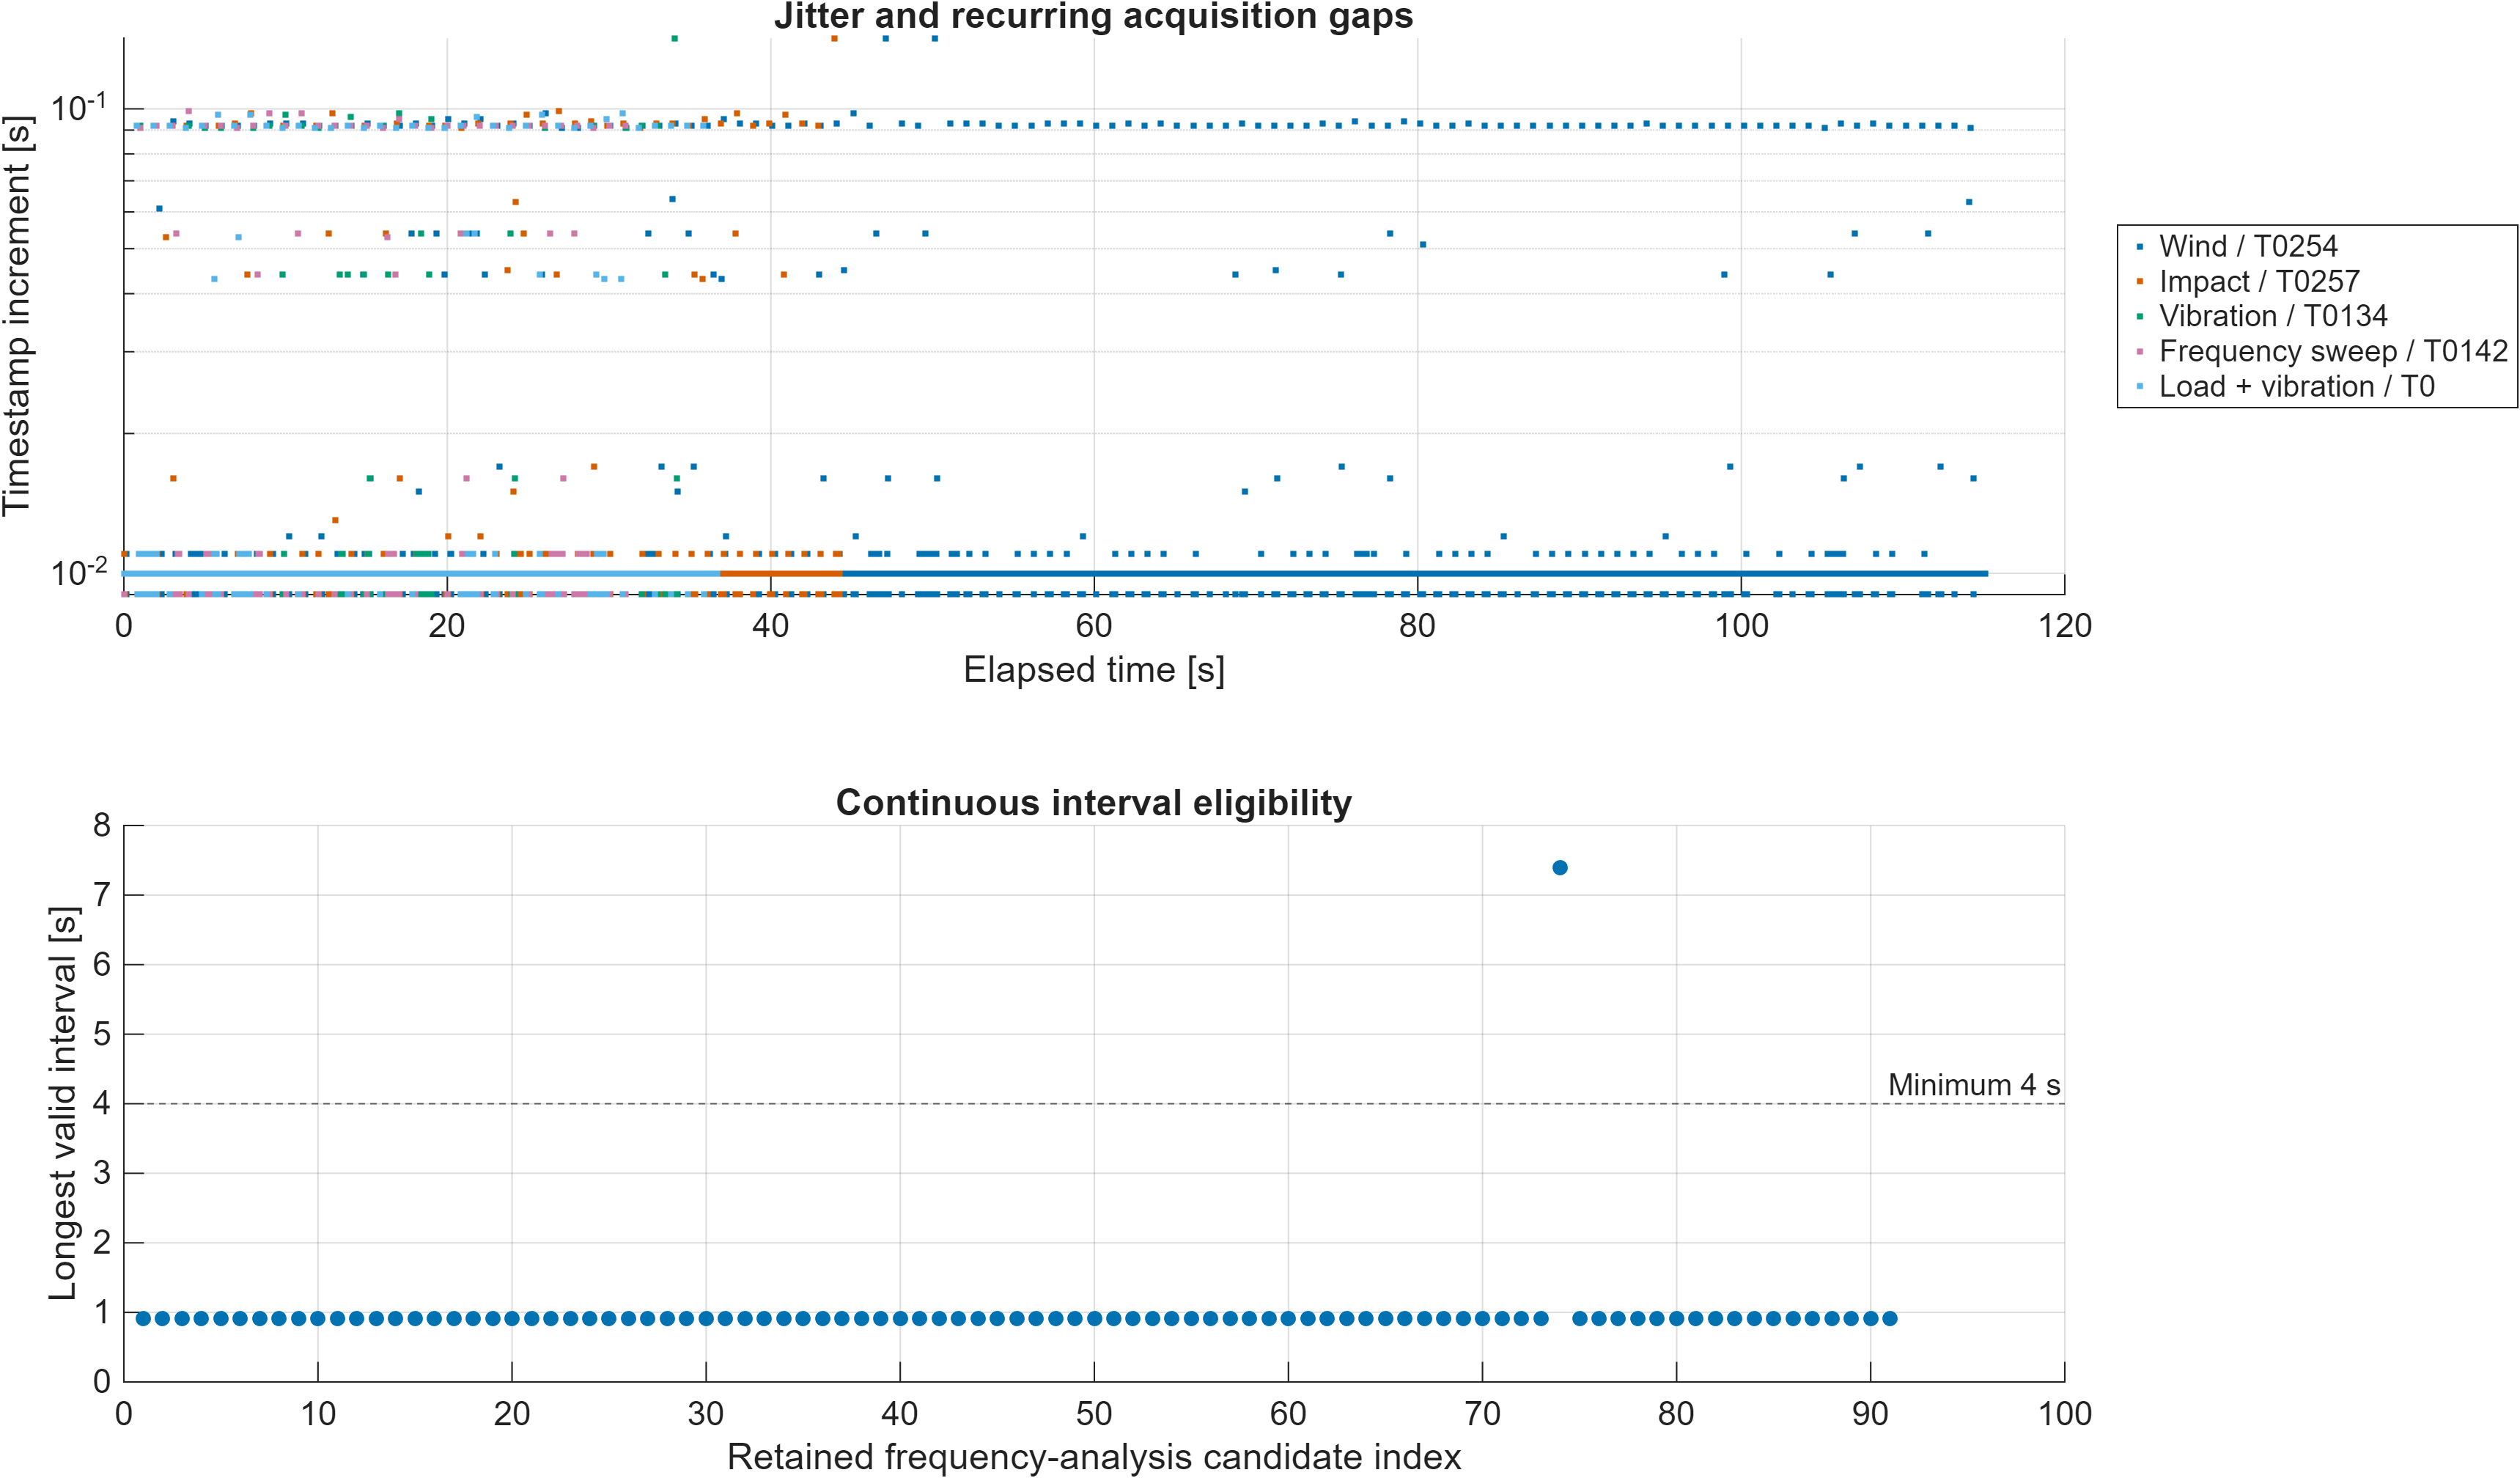
\includegraphics[width=\textwidth,height=0.37\textheight,keepaspectratio]{figures/F16_timestamp_integrity.png}
\caption{Timestamp increments in representative runs and the longest continuous valid intervals in all candidates.}\label{fig:F16}
\end{figure}
Only 1 of 91 candidates passes the unchanged continuity screen. T0236 supplies a 7.399 s interval; the other candidates have maximum continuous spans no longer than 0.912 s. Recurrent acquisition gaps, rather than a low nominal sampling rate, therefore constrain frequency analysis. Interpolating through those gaps would introduce assumptions about unmeasured vibration. The isolated accepted interval permits a response spectrum, but it cannot establish spectral repeatability across PWM, load or position.\par

\renewcommand{\thefigure}{F17}
\begin{figure}[H]\centering
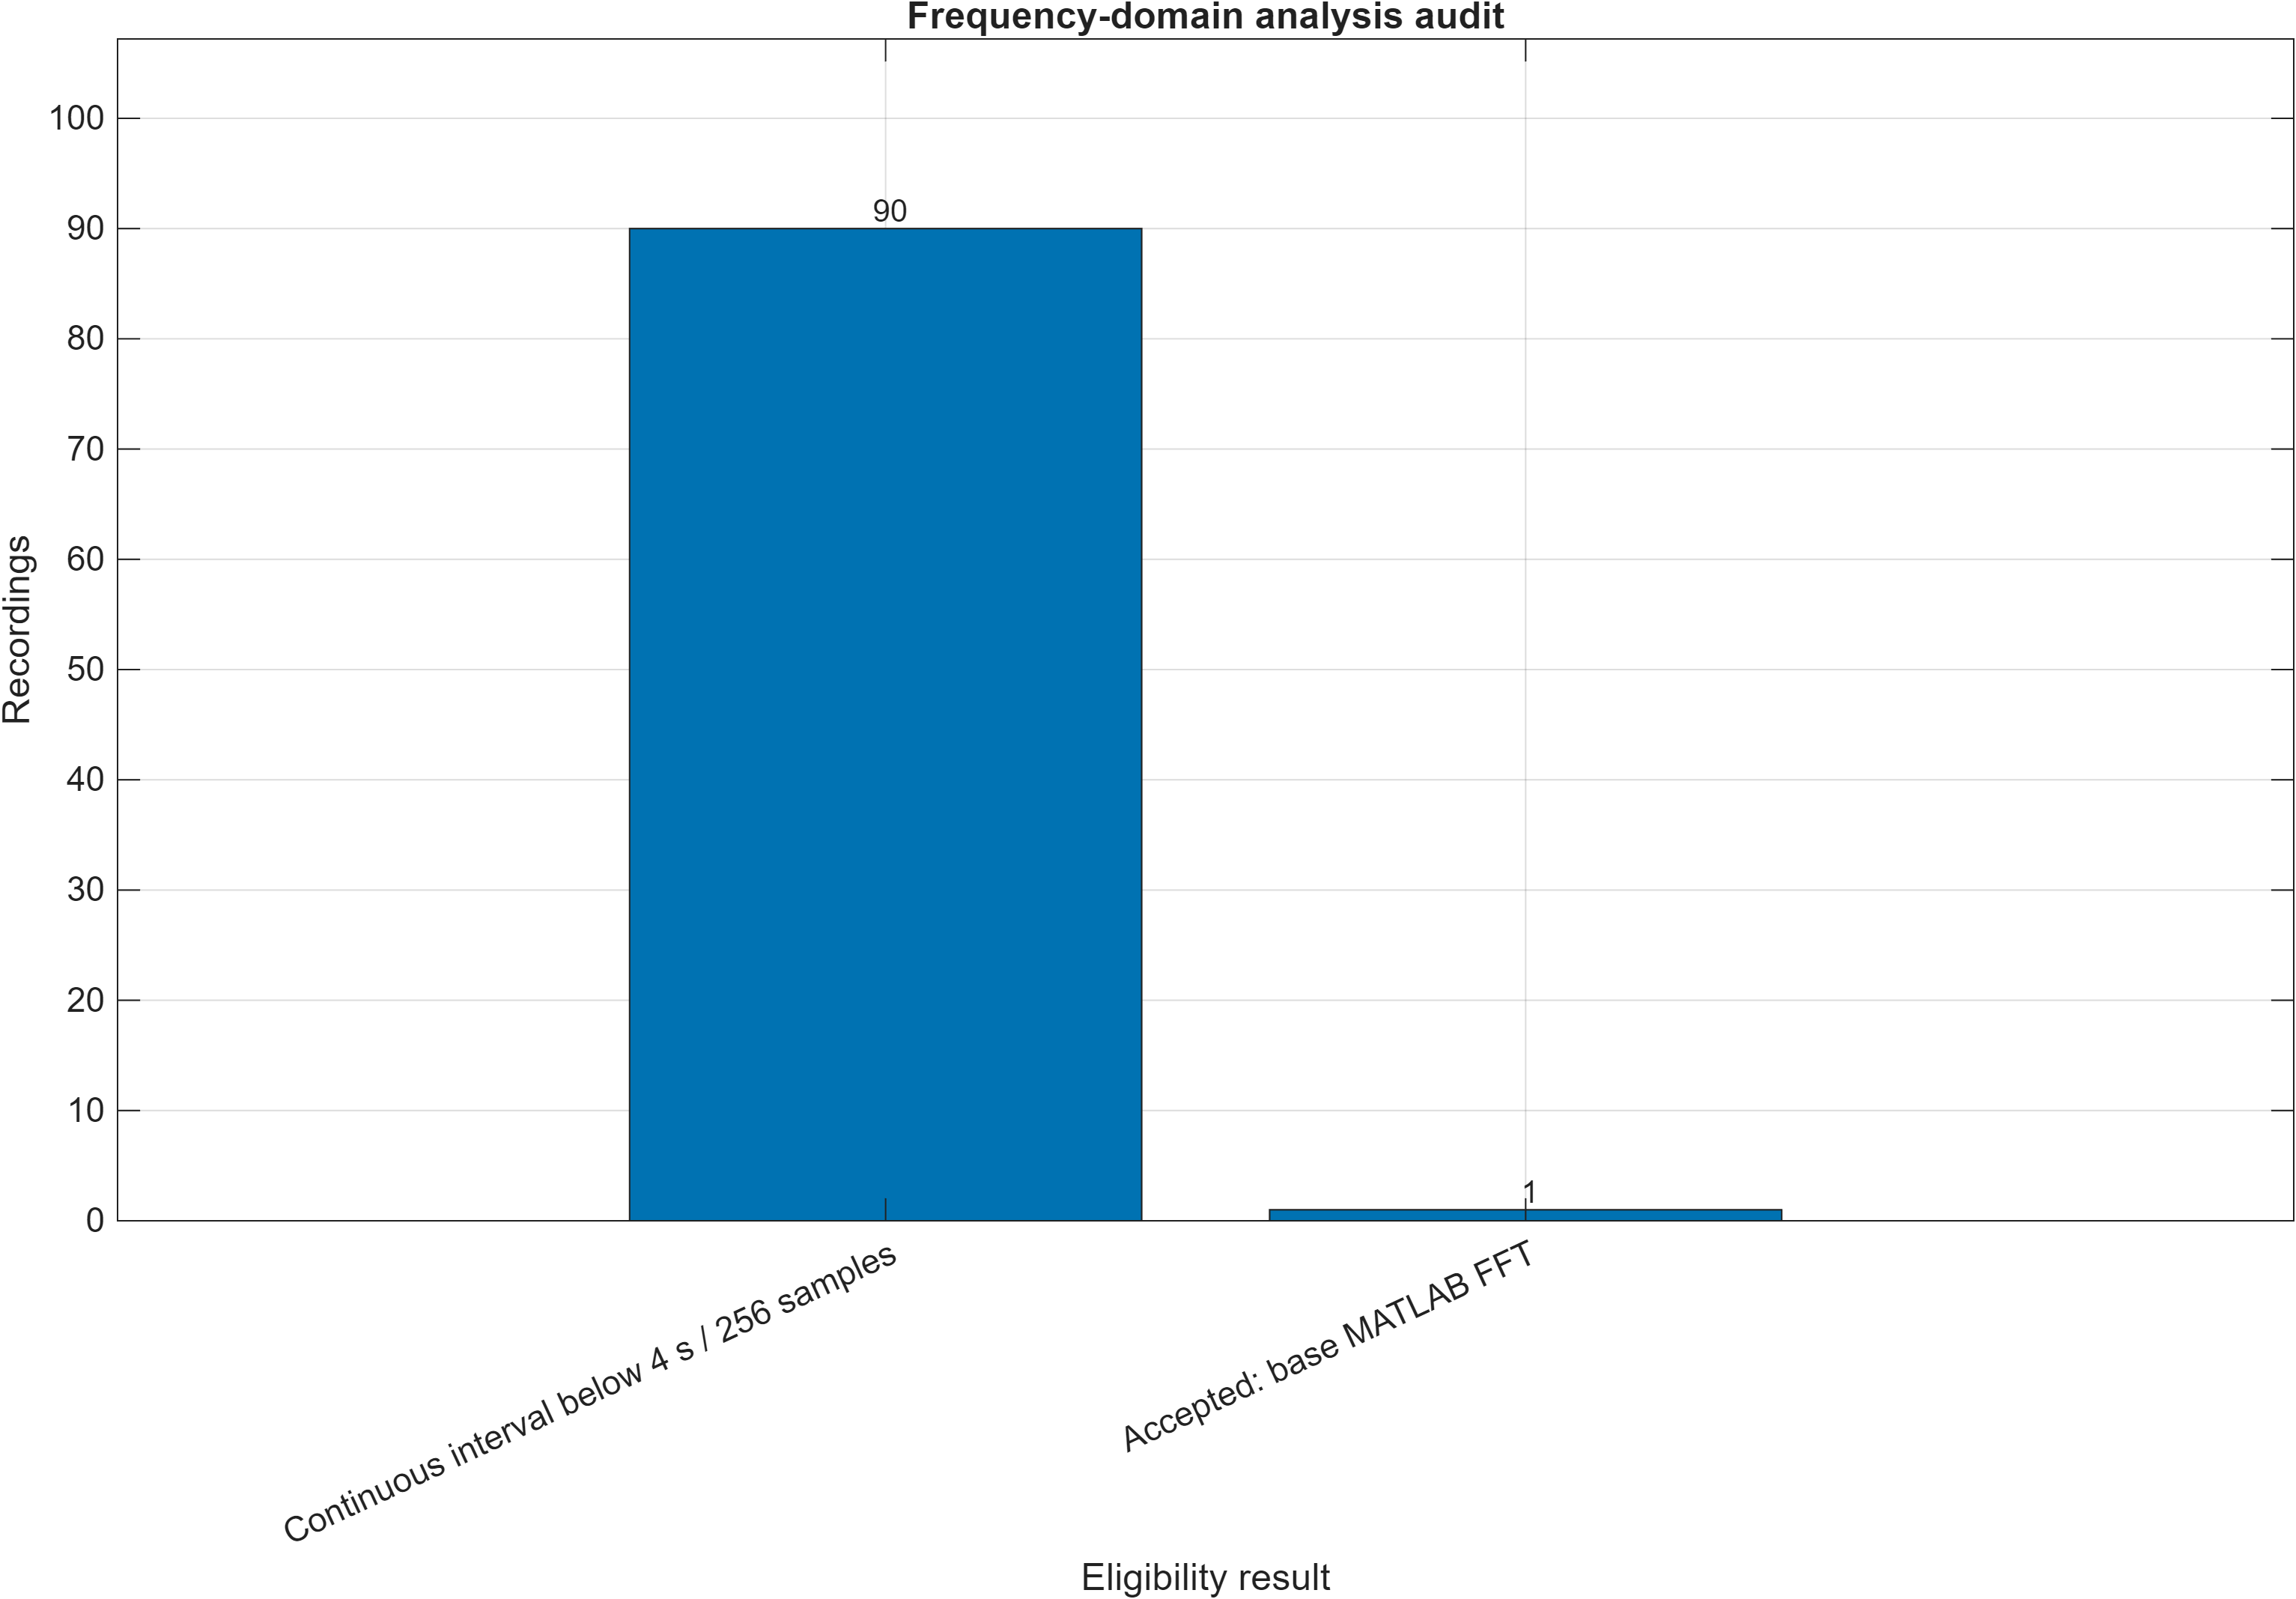
\includegraphics[width=\textwidth,height=0.37\textheight,keepaspectratio]{figures/F17_spectral_eligibility.png}
\caption{Reasons for admitting or withholding frequency-domain analysis.}\label{fig:F17}
\end{figure}
The audit now distinguishes data eligibility from software availability: 90 candidates fail timing and 1 passes for base-MATLAB FFT. The earlier rejection of the valid interval was an unnecessarily restrictive toolbox gate, not a defect in its timestamps. A directly evaluated periodic Hann window and built-in fft recover that result without changing the continuity thresholds. Welch PSD and spectrograms remain omitted because their toolbox functions are not installed; unavailable software is not used to excuse invalid timing elsewhere.\par

\renewcommand{\thefigure}{F33}
\begin{figure}[H]\centering
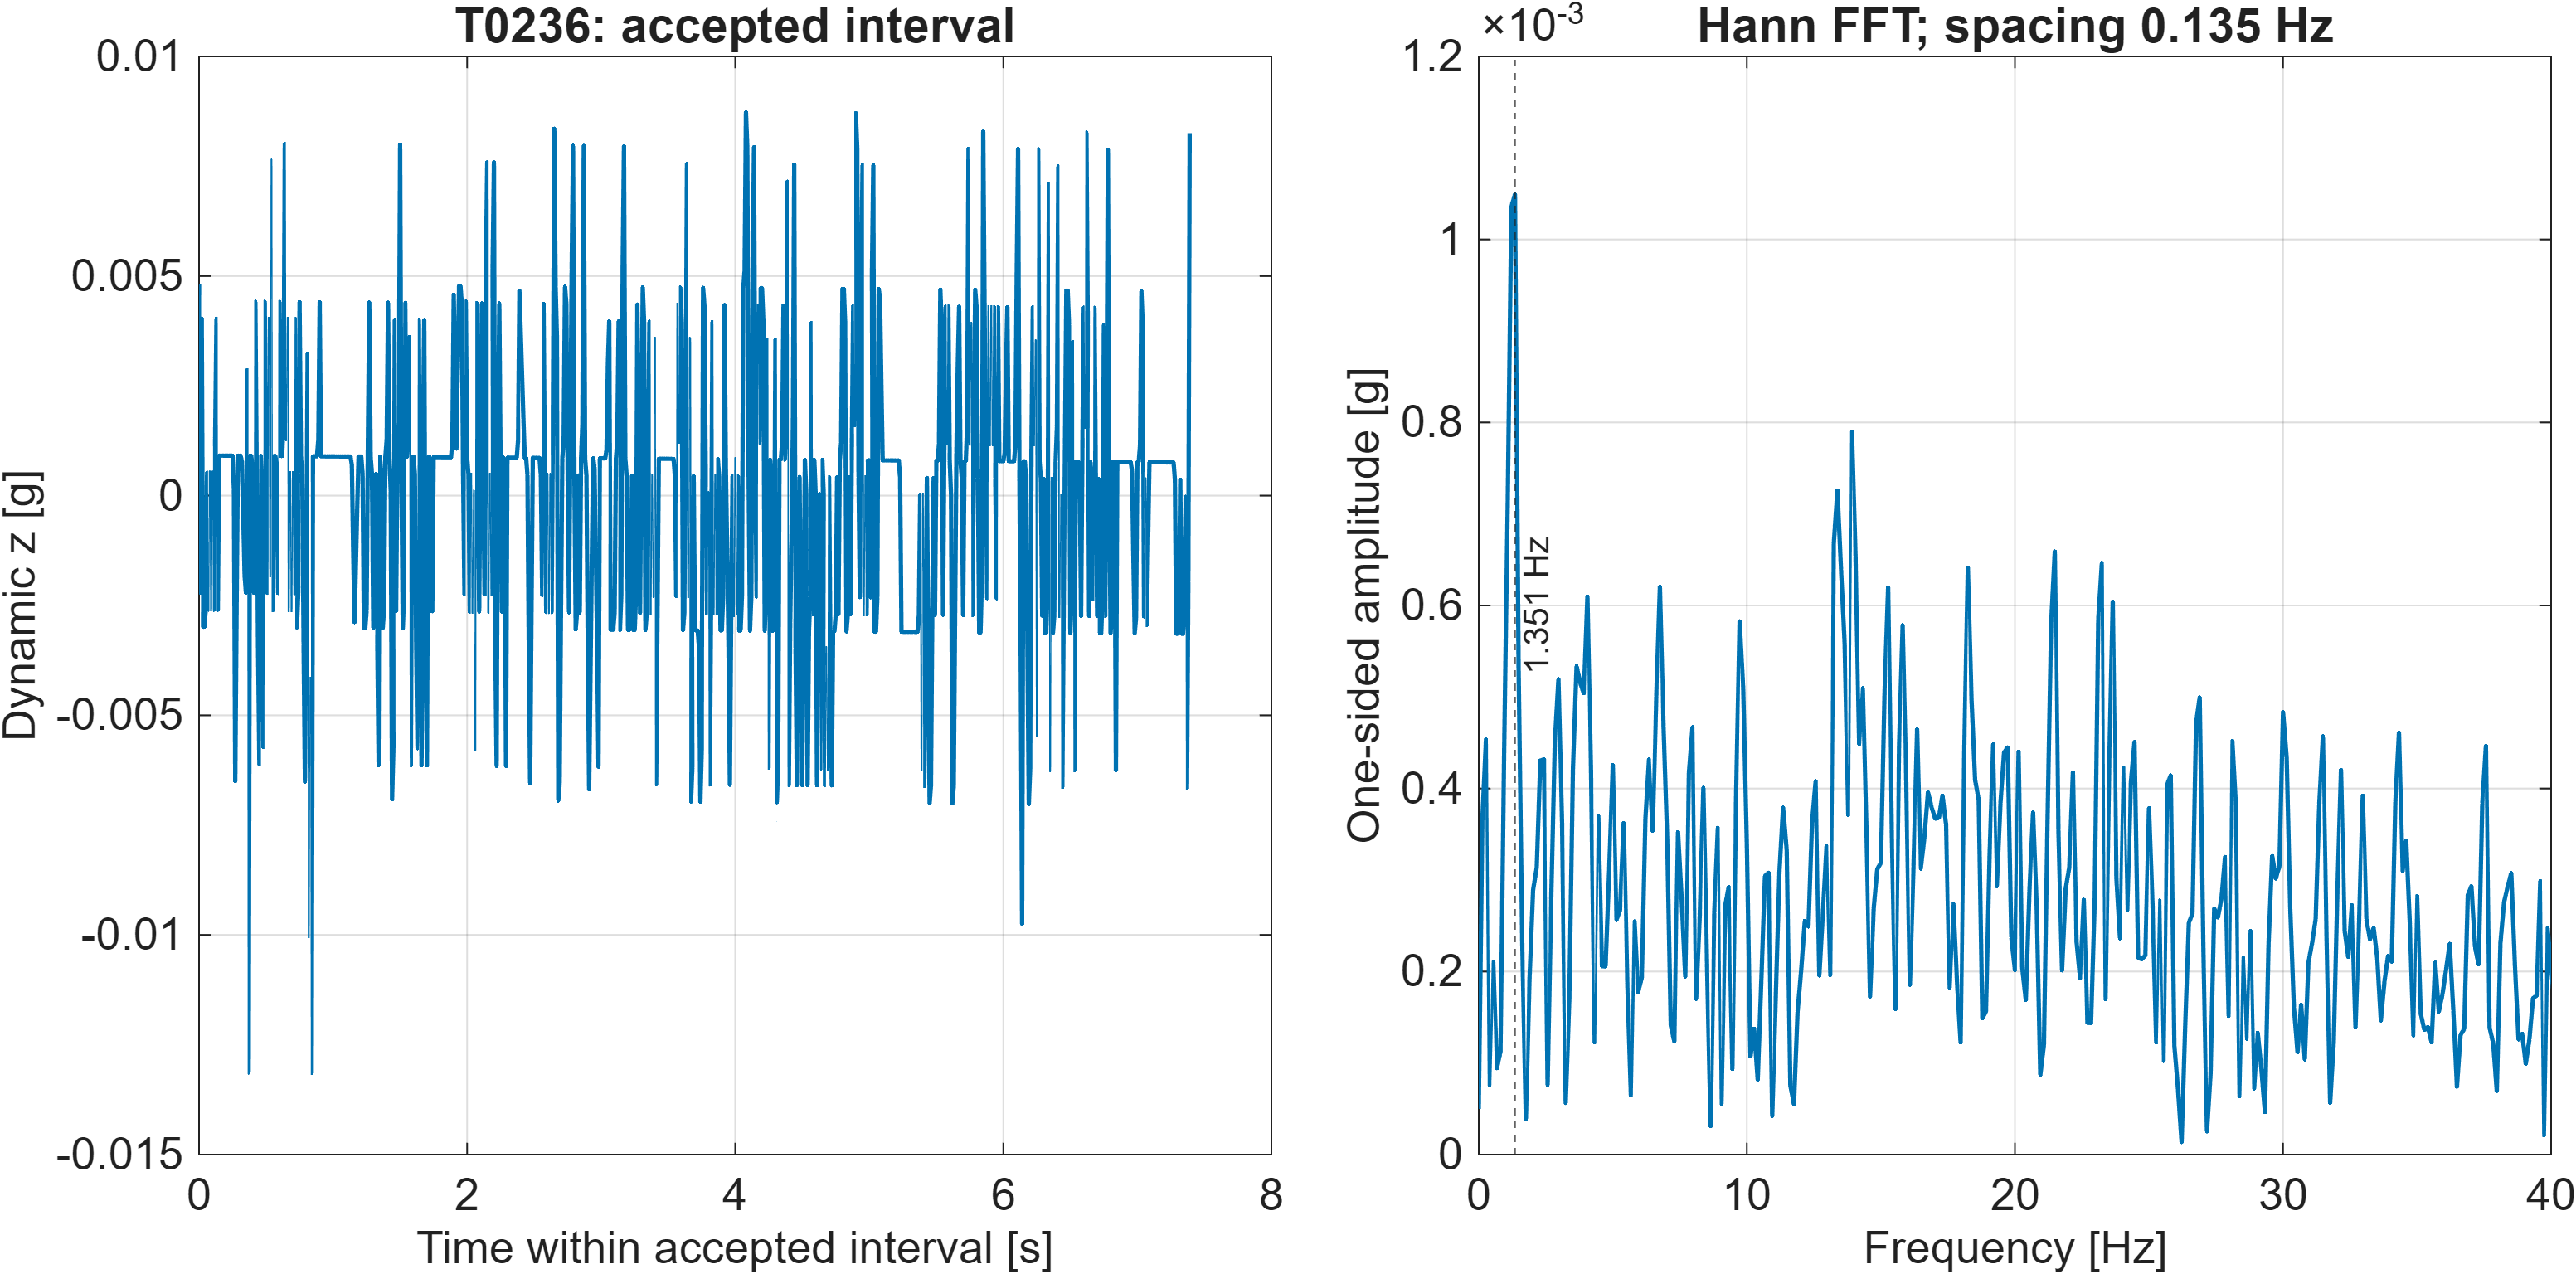
\includegraphics[width=\textwidth,height=0.37\textheight,keepaspectratio]{figures/F33_T0236_base_matlab_fft.png}
\caption{T0236 response spectrum: 13.106--20.505 s, fs 100 Hz, N=740, bin spacing 0.135135 Hz.}\label{fig:F33}
\end{figure}
The accepted interval contains 741 source samples and 740 uniformly resampled values at 100.000 Hz. Its 7.399 s source span yields FFT bin spacing 0.1351 Hz. The largest searched response bin is 1.3514 Hz at 0.001049 g, but the adjacent 1.2162 Hz bin is only 1.3 percent smaller. These bins lie within one Hann main lobe, so the result supports a broad low-frequency response region, not two resolved tones or a uniquely identified structural mode. First/second-half dynamic RMS is 0.00317/0.00348 g, indicating some within-interval variation. Slow modulation, structural motion or excitation variability are plausible; PWM 64 supplies no physical frequency calibration. With no input force, temperature data or independent repeat spectrum, neither resonance nor damping is validated.\par

\Needspace{5\baselineskip}
\section{Combined Load and Vibration Effects}
The September 25 series supports comparisons across applied mass, position and PWM within one acquisition batch. A 0.25 kg subset also supports vibration-disabled versus vibration-enabled comparisons at matching position. The retained dataset has no matching unloaded vibration baseline in this batch, so cross-batch unloaded and loaded recordings are not used to claim a loading effect.

\renewcommand{\thefigure}{F18}
\begin{figure}[H]\centering
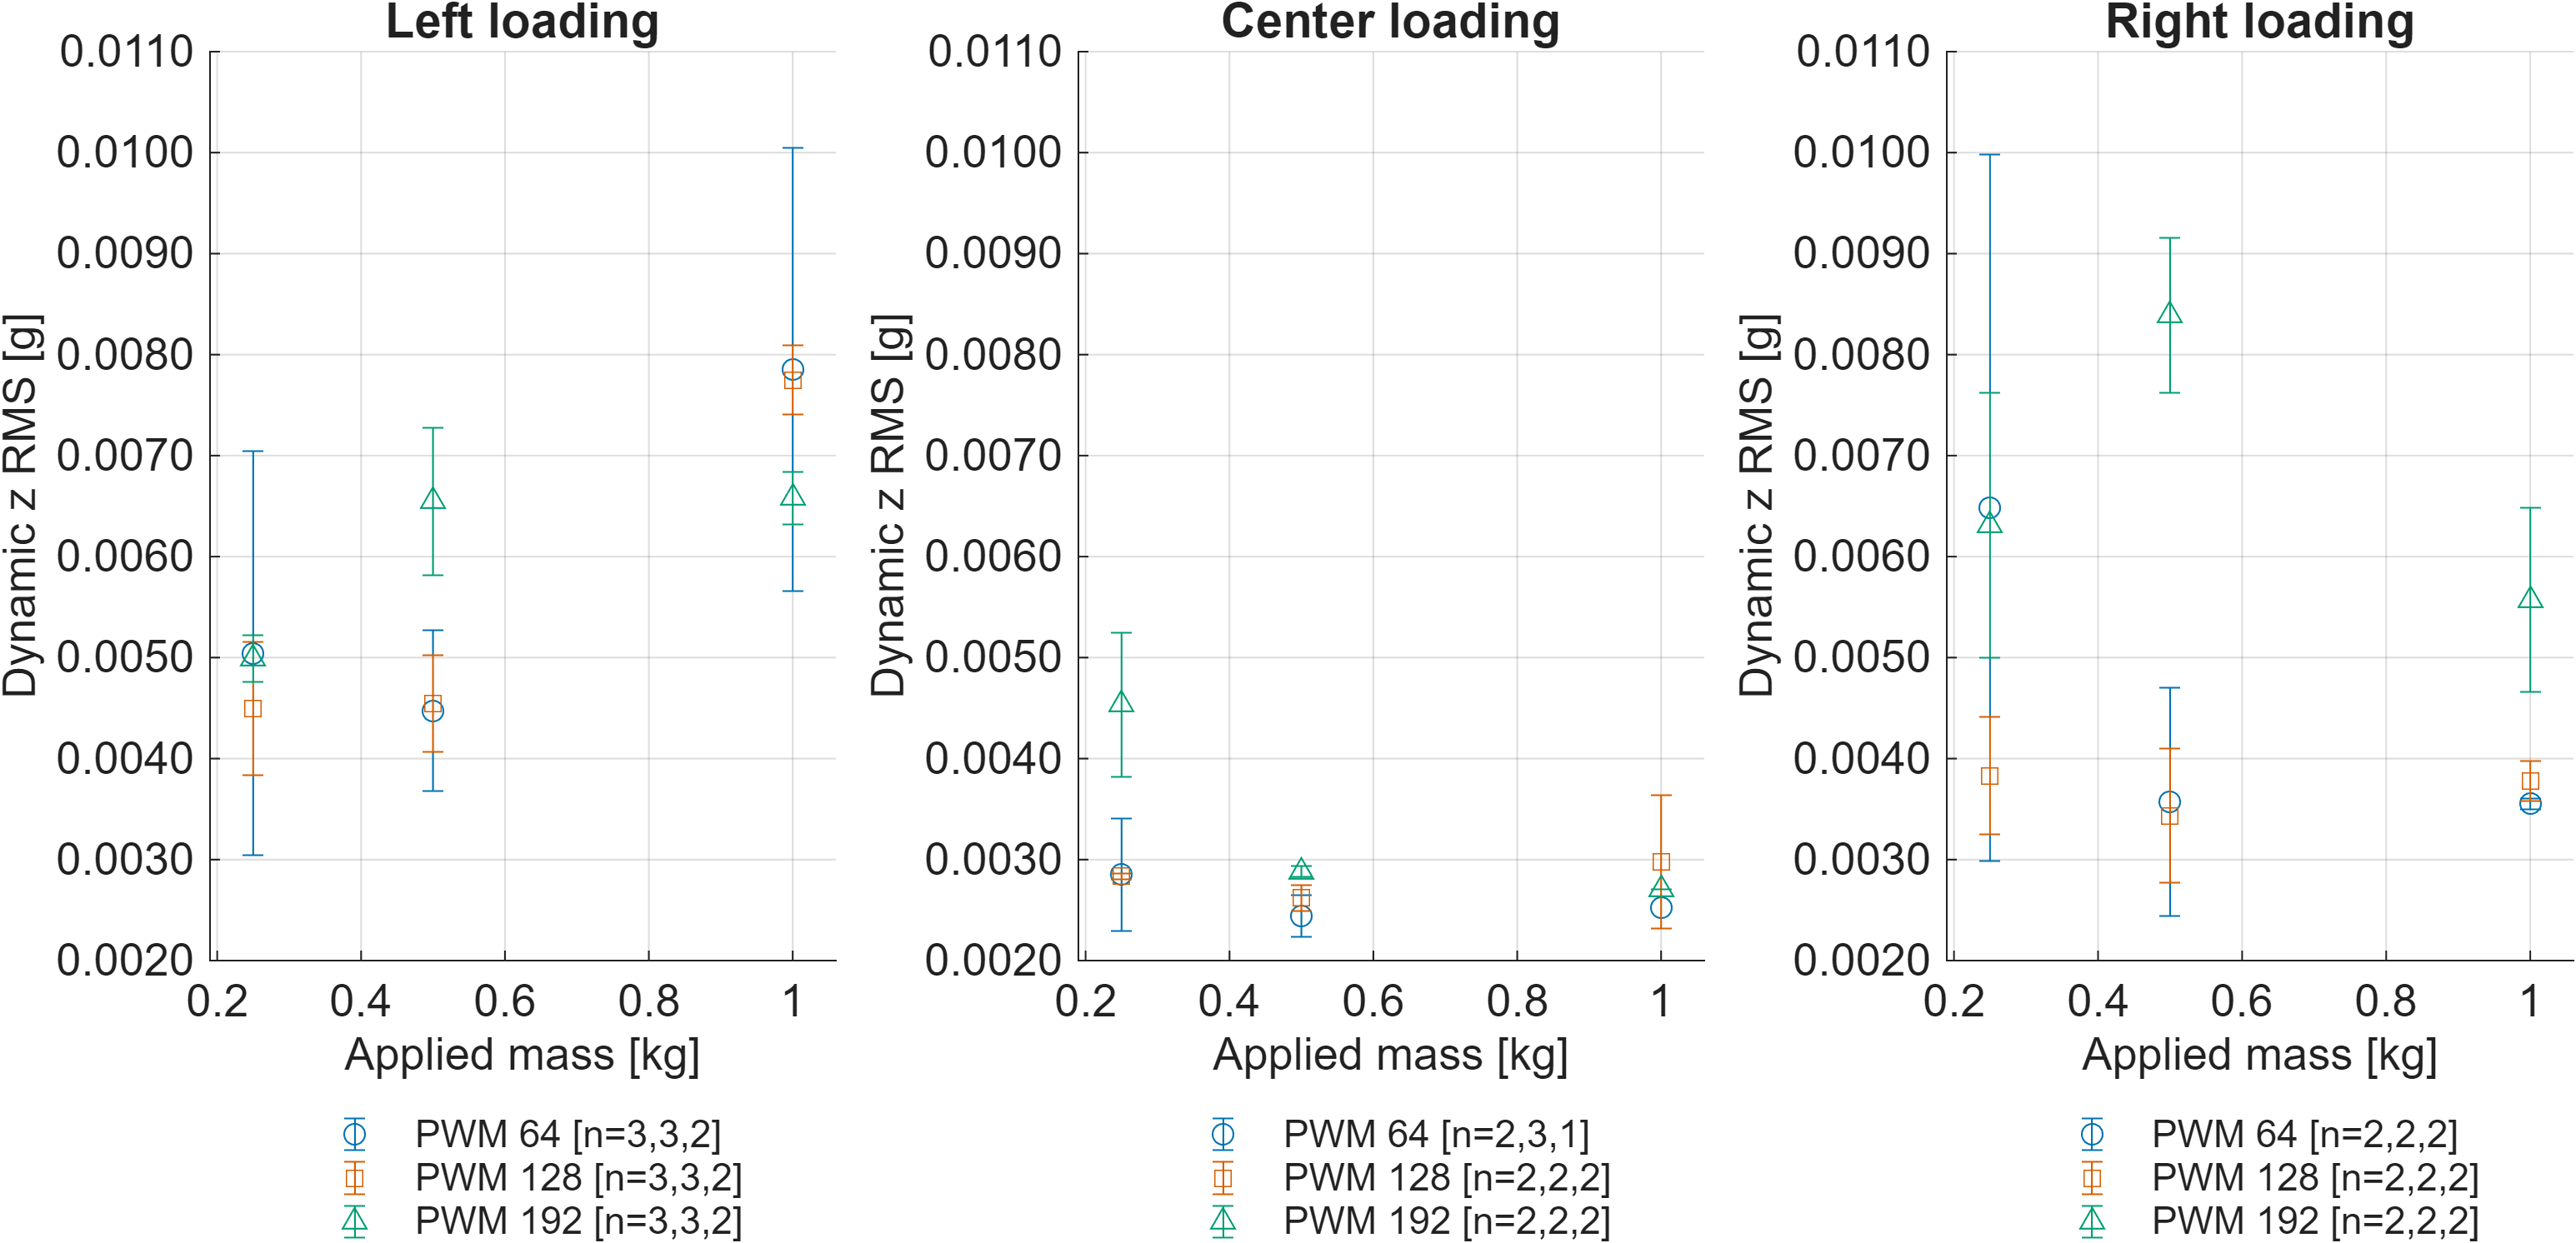
\includegraphics[width=\textwidth,height=0.37\textheight,keepaspectratio]{figures/F18_combined_rms_mass.png}
\caption{Acceleration RMS versus mass within matching position and PWM strata of September 25.}\label{fig:F18}
\end{figure}
Loading does not produce a universal increase in vibration response. At left loading/PWM 64, mean RMS changes 0.00504 to 0.00447 to 0.00785 g as mass increases from 0.25 to 0.5 to 1 kg: a 11.3 percent decrease followed by a 75.6 percent increase. At center/PWM 192, the endpoint change instead decreases 40.3 percent. Changes in mass distribution, contact conditions or excitation coupling could alter the measured dynamics in either direction; the data do not isolate those mechanisms. The left/PWM 64 repetition spread is large, and one center/1 kg/PWM 64 condition has only a single recording. Thus mass must be interpreted together with position and command, and neither a monotonic mass law nor a resonance shift is established.\par

\renewcommand{\thefigure}{F19}
\begin{figure}[H]\centering
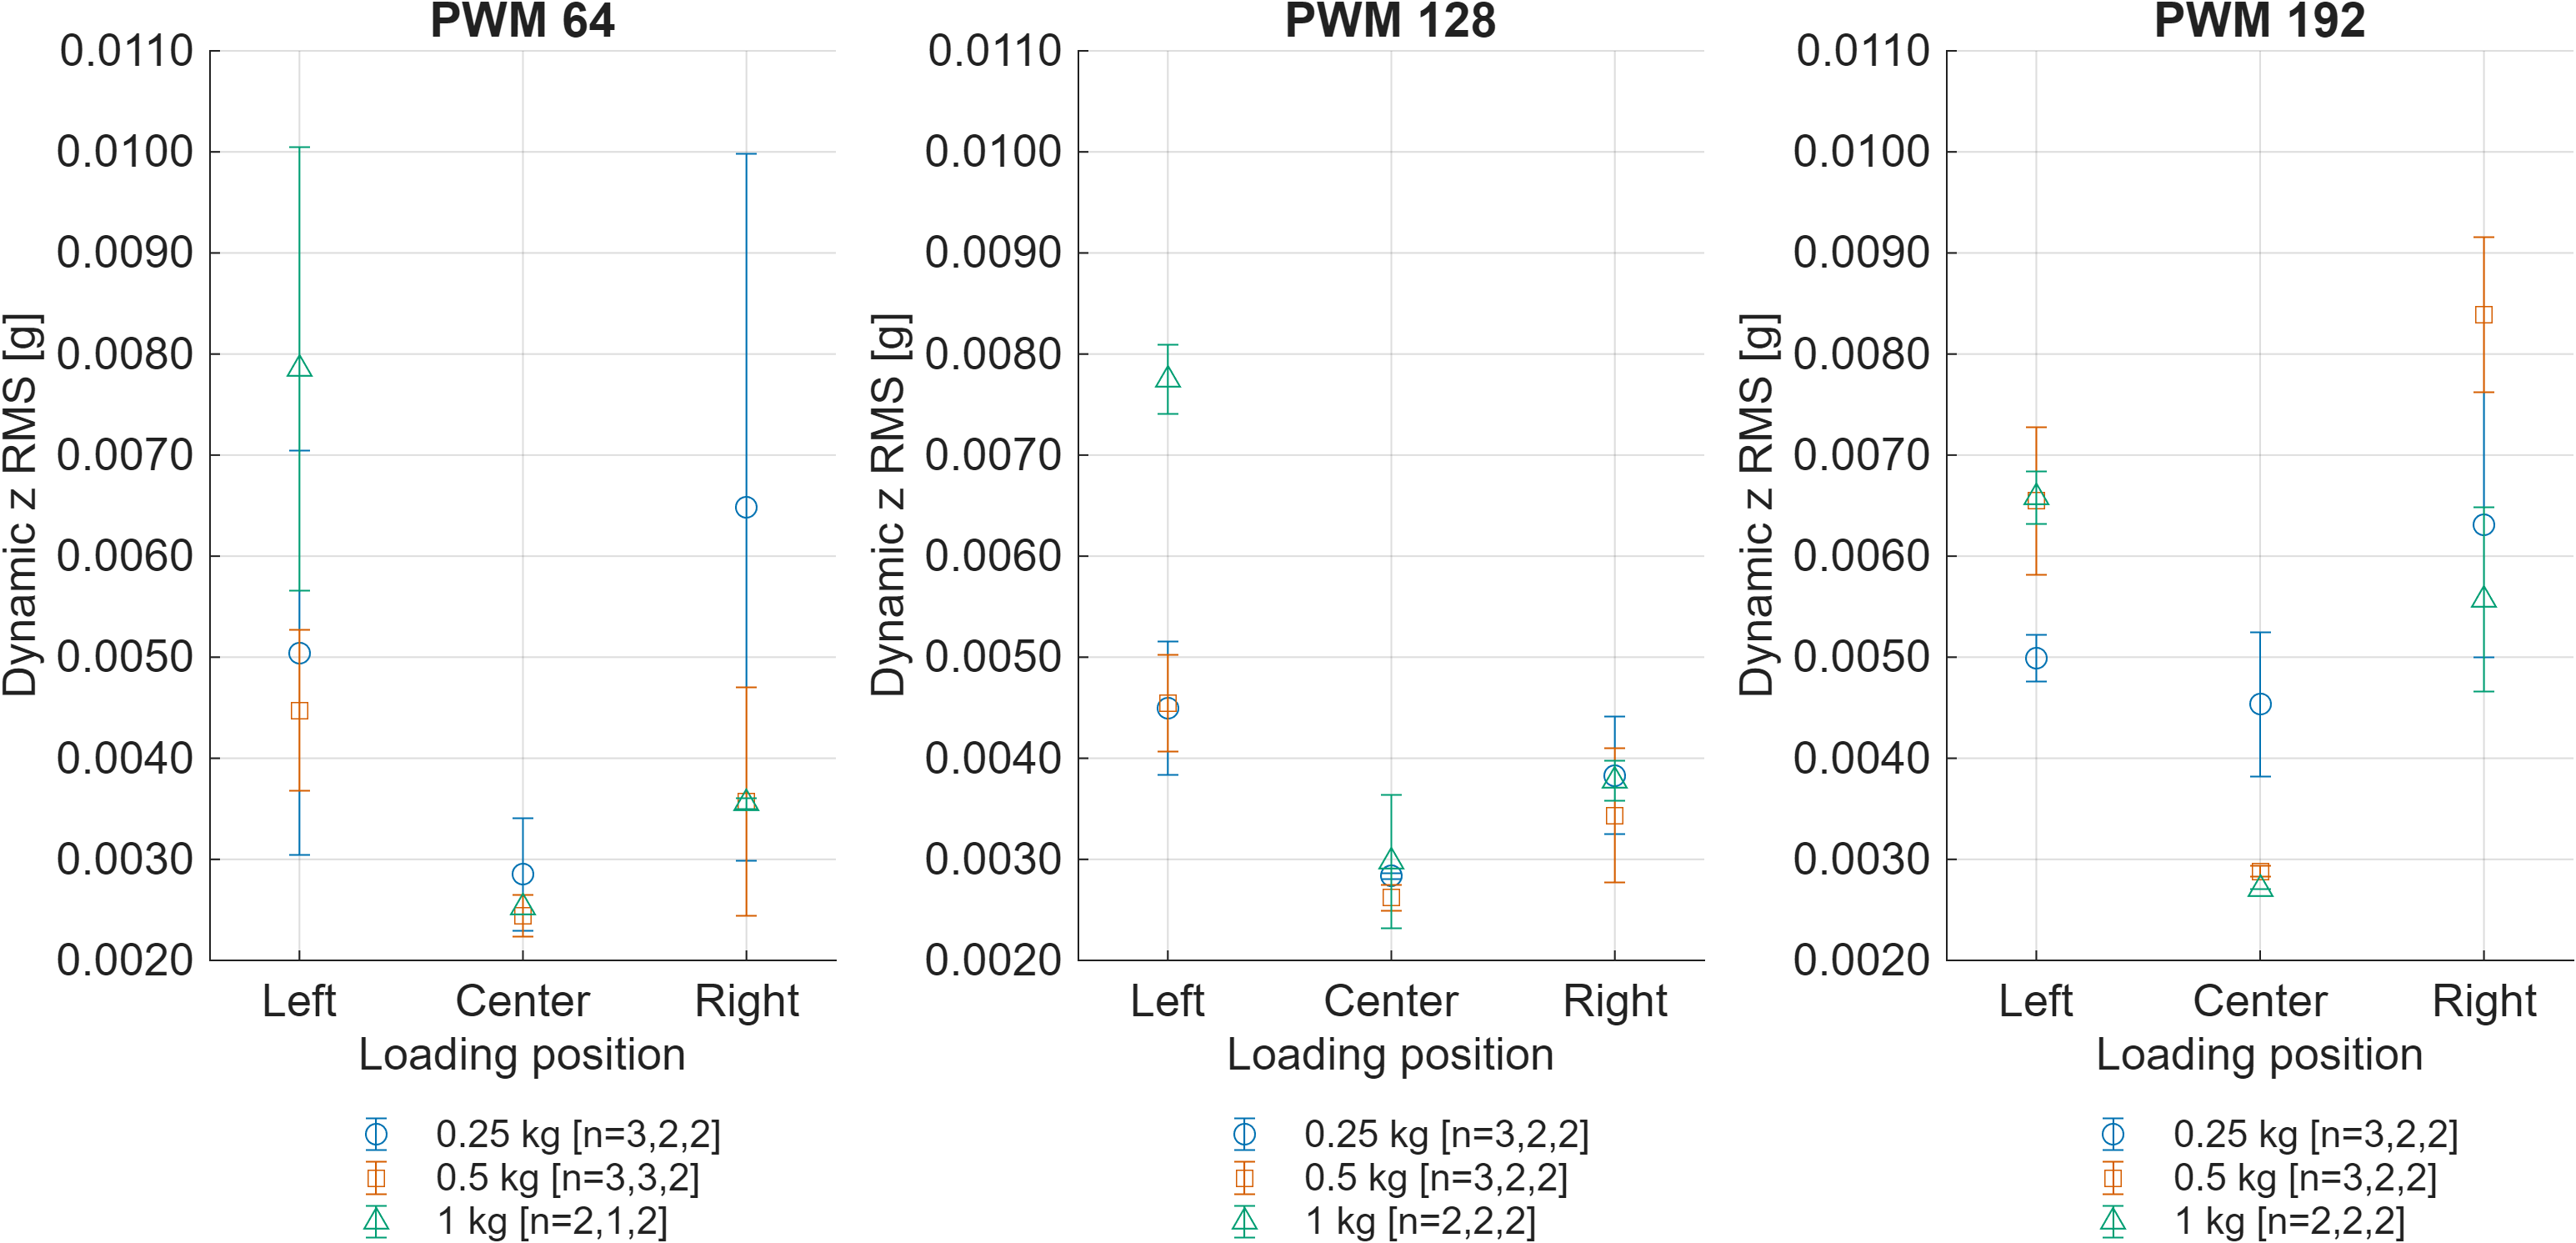
\includegraphics[width=\textwidth,height=0.37\textheight,keepaspectratio]{figures/F19_combined_rms_position.png}
\caption{Position sensitivity of vibration RMS at matching mass and PWM.}\label{fig:F19}
\end{figure}
Center loading gives the smallest mean z RMS in all 9 matched mass/PWM combinations. For example, at 0.5 kg/PWM 128, left/center/right means are 0.00455/0.00262/0.00344 g, placing center 42.4 percent below left and 23.7 percent below right. This repeated ordering is stronger descriptive evidence of position sensitivity than a pooled mass trend. Load placement may alter local motion, load transfer or coupling between the motor and bridge, but the sensor location and input force are insufficiently characterized to identify a mechanism or modal node. Common vertical scales make the comparison explicit. Small repetition counts and variable scatter at the edge positions still require independent replication before position-dependent dynamic predictions can be validated.\par

\renewcommand{\thefigure}{F20}
\begin{figure}[H]\centering
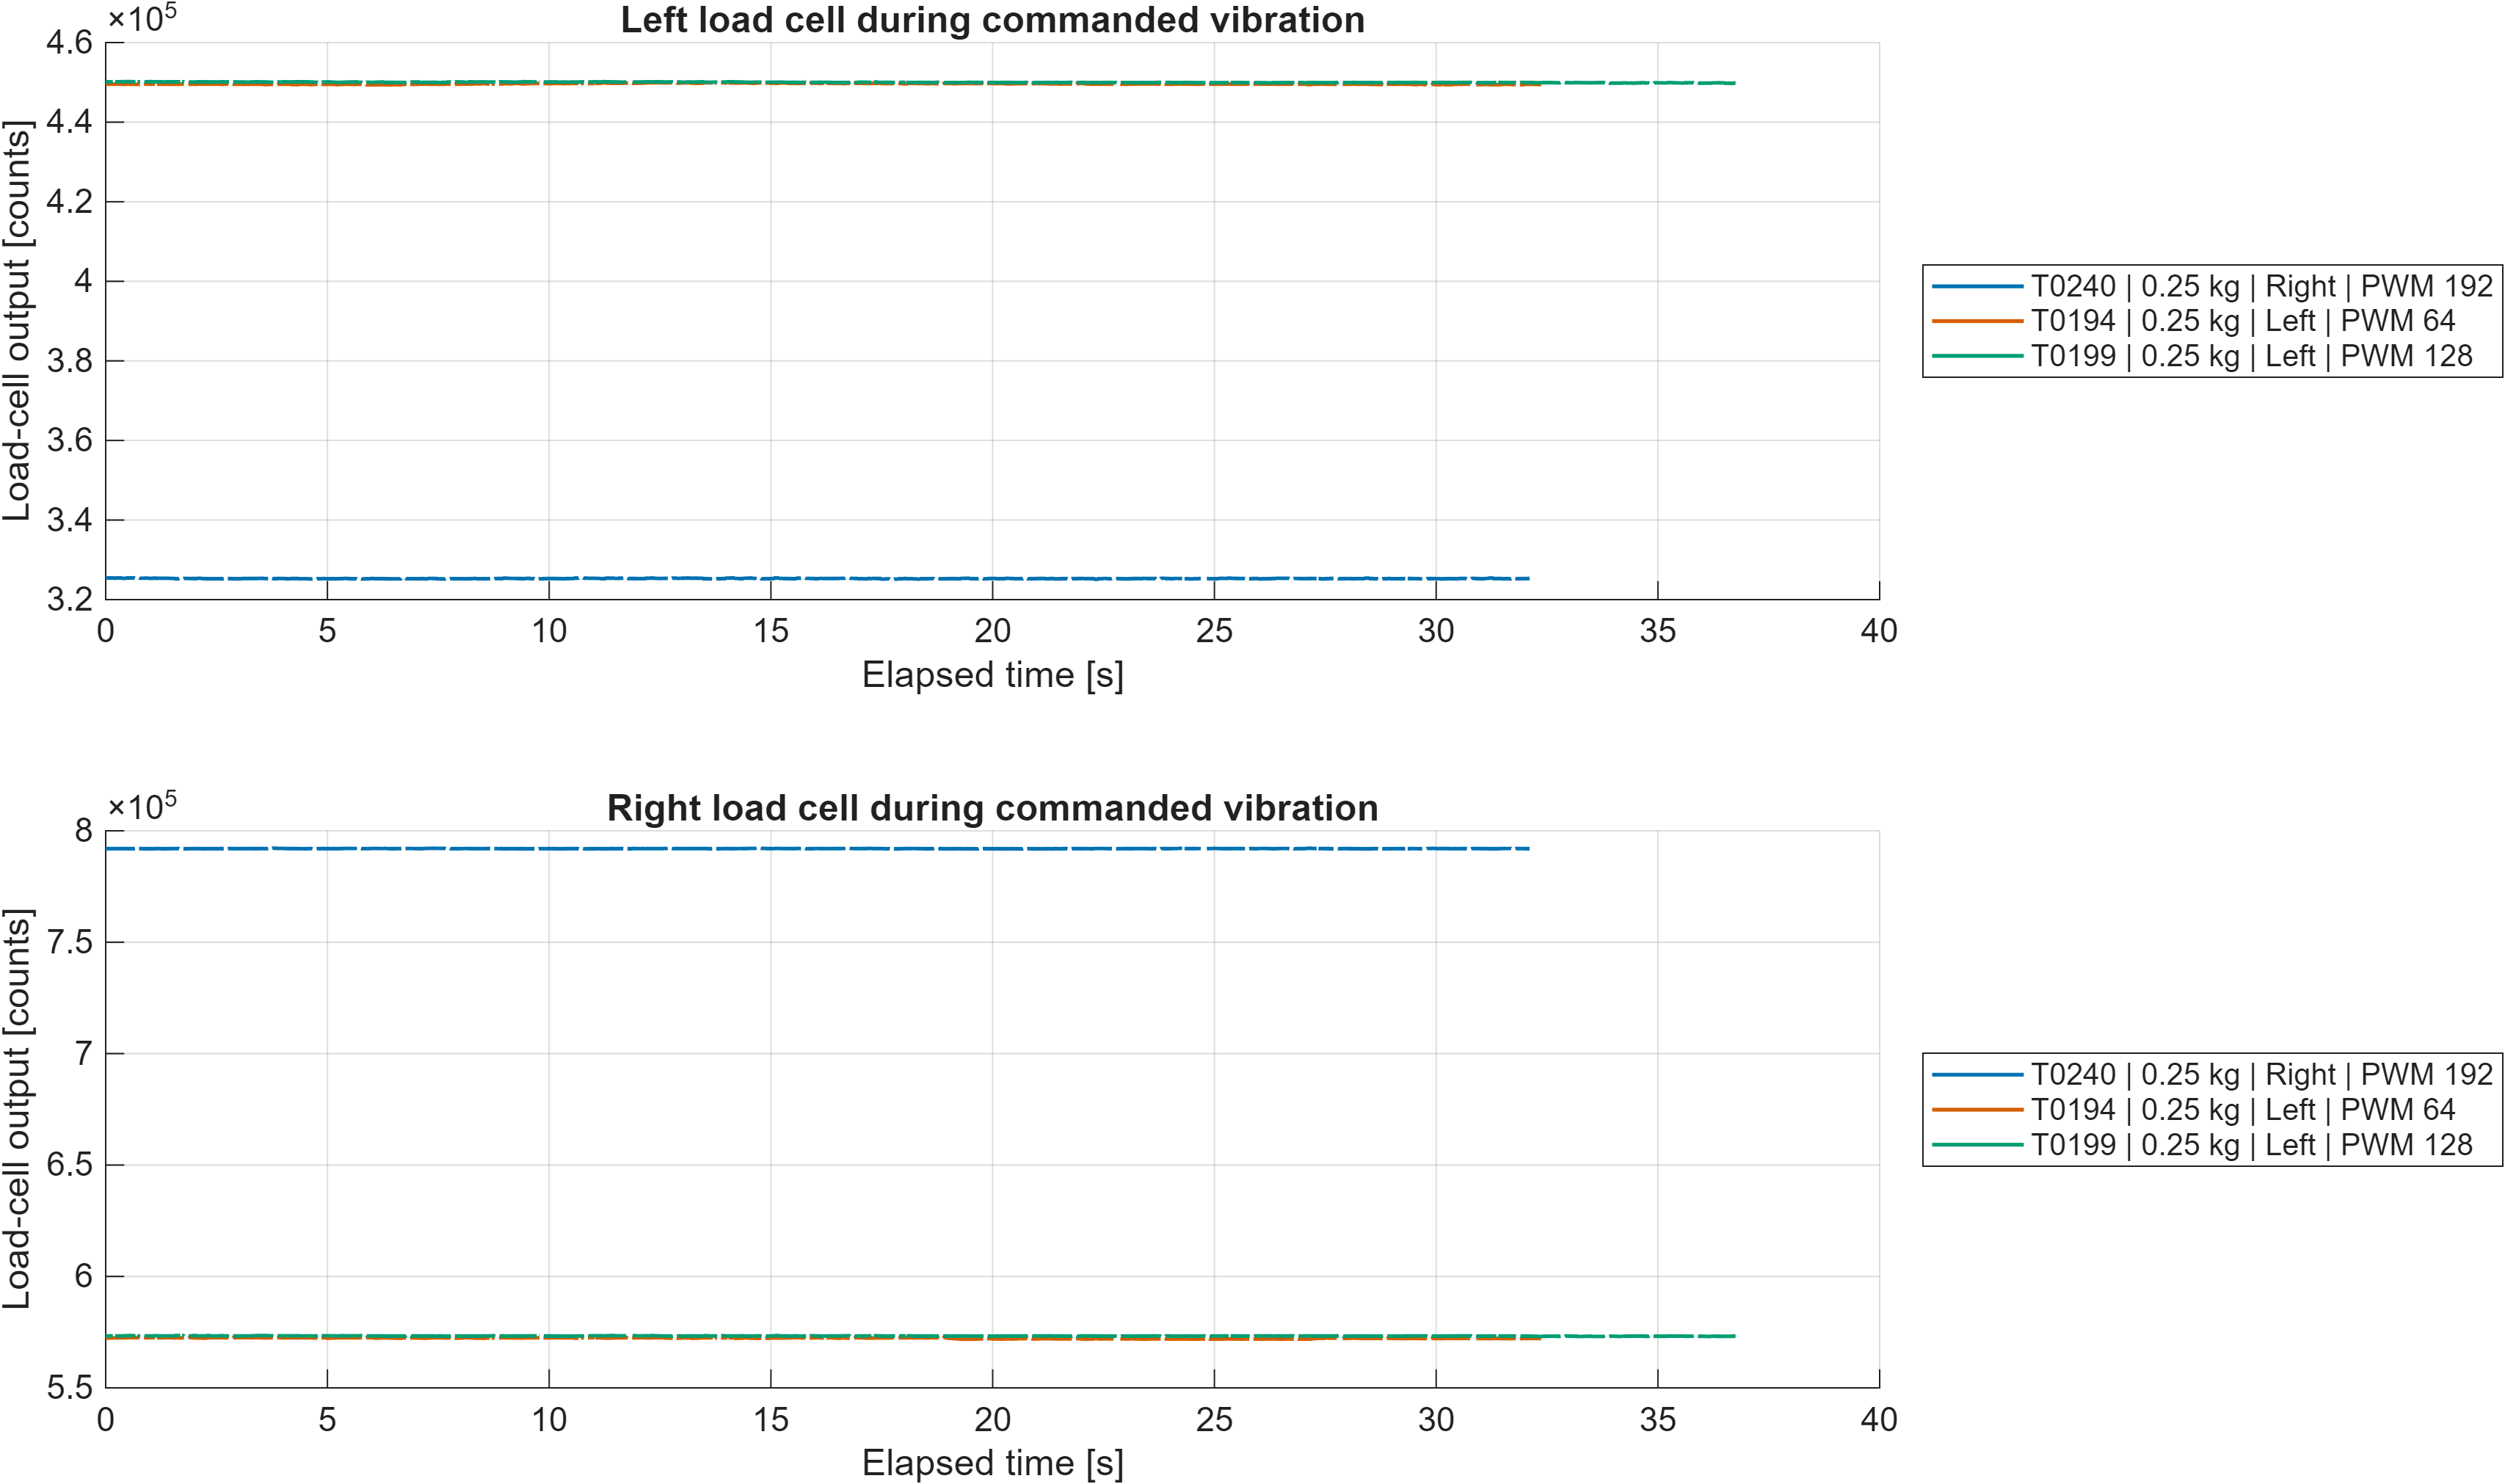
\includegraphics[width=\textwidth,height=0.37\textheight,keepaspectratio]{figures/F20_combined_loadcell_histories.png}
\caption{Representative load-cell histories during combined loading and vibration.}\label{fig:F20}
\end{figure}
The representative load-cell levels remain strongly separated by position during commanded vibration. The right-loaded representative has a left-cell median of 325295 counts, whereas the two left-loaded representatives span 449571--449982 counts. The opposite-channel levels reverse this spatial contrast. Their nearly steady raw baselines indicate that the plotted scale is dominated by sustained loading and sensor offsets, not by the much smaller acceleration fluctuations. The figure cannot isolate PWM because the PWM 192 example is right-loaded and the lower-command examples are left-loaded. Moreover, apparent flatness at this scale does not prove zero dynamic load. Calibrated, sufficiently fast load-cell acquisition and matched-position comparisons would be required to quantify vibration-induced support-force variation.\par

\renewcommand{\thefigure}{F21}
\begin{figure}[H]\centering
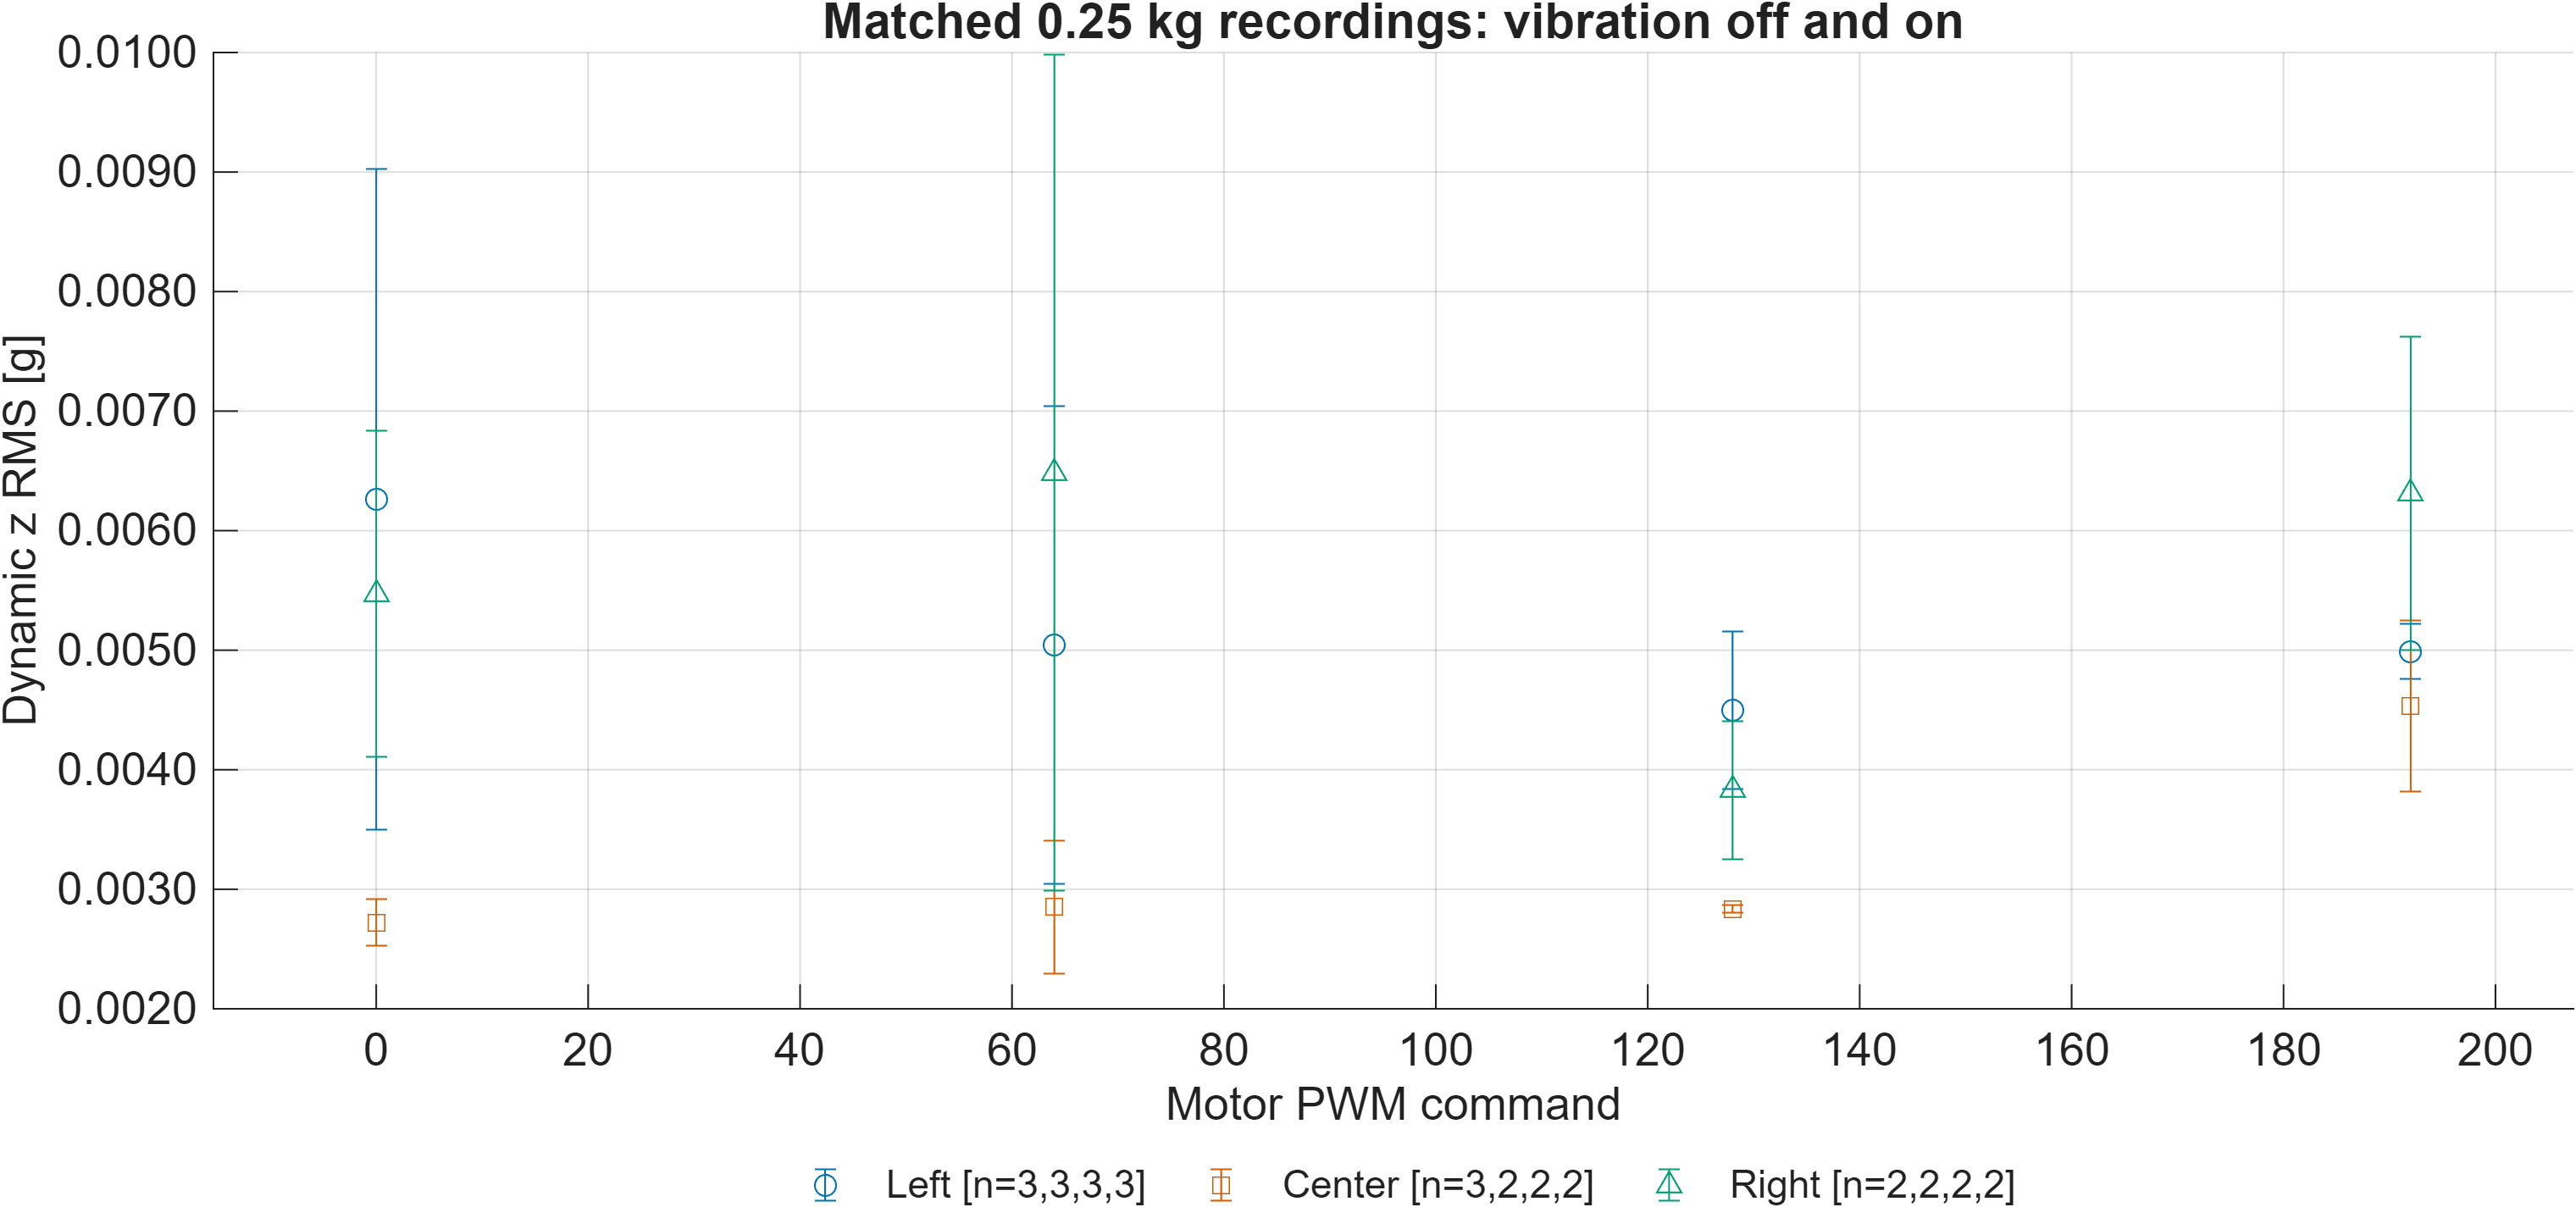
\includegraphics[width=\textwidth,height=0.37\textheight,keepaspectratio]{figures/F21_matched_vibration_off_on.png}
\caption{Same-batch 0.25 kg comparison of vibration-disabled and vibration-enabled recordings.}\label{fig:F21}
\end{figure}
The matched 0.25 kg off/on comparison is directionally inconsistent. At PWM 192 relative to PWM 0, mean RMS changes by -20.3 percent at left, +66.6 percent at center and +15.4 percent at right. The left decrease is counterintuitive if motor operation is assumed to add a fixed independent vibration component, but the off-run standard deviation (0.00276 g) is large relative to that difference. Center increases from 0.00272 to 0.00453 g and shows a clearer descriptive separation. Different ambient motion, mounting or intermittent excitation could explain part of the variability. These are separate runs, not paired before/after measurements; the OFF condition is not guaranteed motionless. The results reject a simple universal command multiplier without proving a causal position effect.\par

\Needspace{5\baselineskip}
\section{Temperature-Induced Sensor Drift}
THERMAL\_01 consists of two recording segments from one session with an approximately five-minute interruption. Each segment has its own elapsed-time axis, starting at its first finite sensor record. No samples are invented and no line crosses the interruption. Part 2 contains an all-missing leading record followed by a 539.826 s timestamp gap; this artifact is distinct from the approximate interruption supplied in the experiment description.

Thermal scatter and drift summaries use occupied one-second median bins, explicitly as summaries rather than a replacement cleaned dataset. Empty bins are not filled. For each sensor, a trend is fitted to paired finite bin summaries only when there are at least 20 bins and a temperature span of at least one degree Celsius. Fits use left temperature as the common measured reference and are computed separately by segment. The reported slopes and coefficients of determination describe observational associations. Temporal autocorrelation, temperature gradients, possible orientation changes, excitation and segment offsets prevent interpreting the fits as a validated compensation model.

\renewcommand{\thefigure}{F22}
\begin{figure}[H]\centering
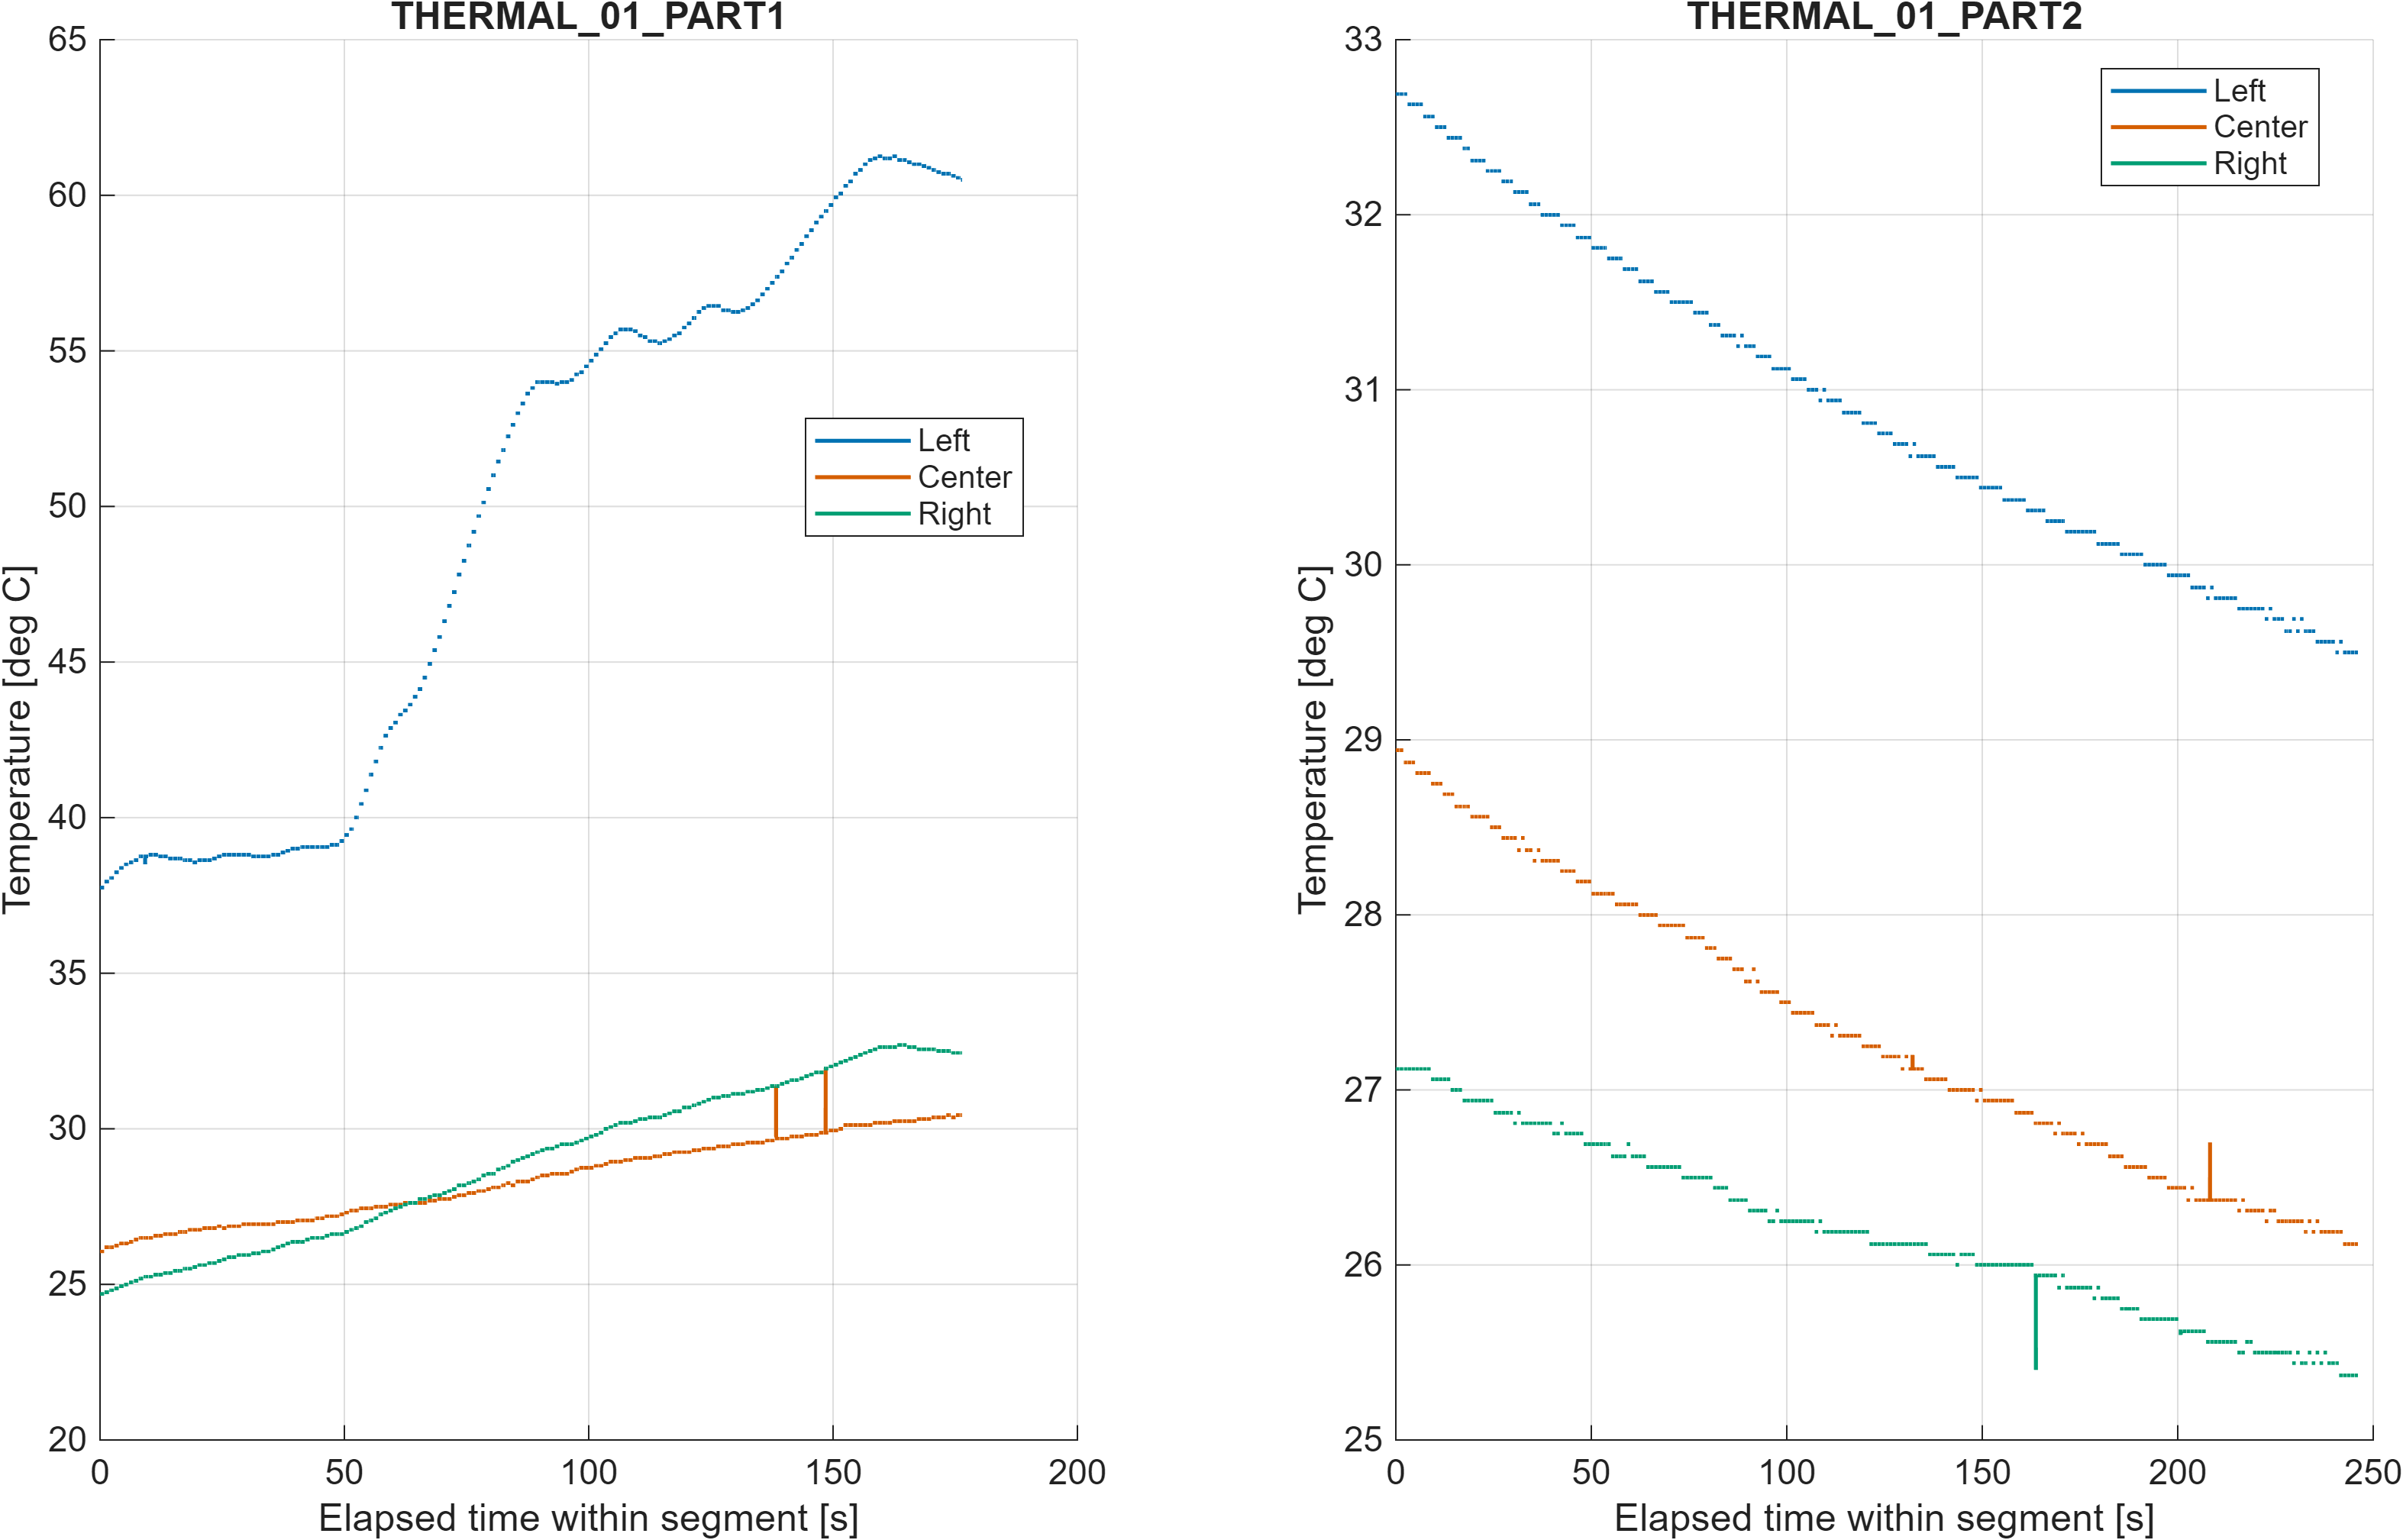
\includegraphics[width=\textwidth,height=0.37\textheight,keepaspectratio]{figures/F22_thermal_temperature.png}
\caption{Temperature channels in separately displayed THERMAL\_01 recording segments.}\label{fig:F22}
\end{figure}
The first segment is predominantly a localized heating observation: first-to-last five-second median temperatures change by +22.50, +4.19 and +7.63 deg C at left, center and right. The second segment cools, with corresponding changes of -3.16, -2.75 and -1.75 deg C. The much larger left-side heating excursion indicates a spatial thermal gradient rather than uniform bridge temperature. Such gradients can influence sensor electronics, mounting stresses and apparent mechanical response differently at each location. Both segments belong to one session, and the missing interruption prevents observing the transition directly. Segment-specific offsets and different temperature ranges therefore preclude treating these data as repeated heating/cooling cycles or identifying hysteresis from a continuous loop.\par

\renewcommand{\thefigure}{F23}
\begin{figure}[H]\centering
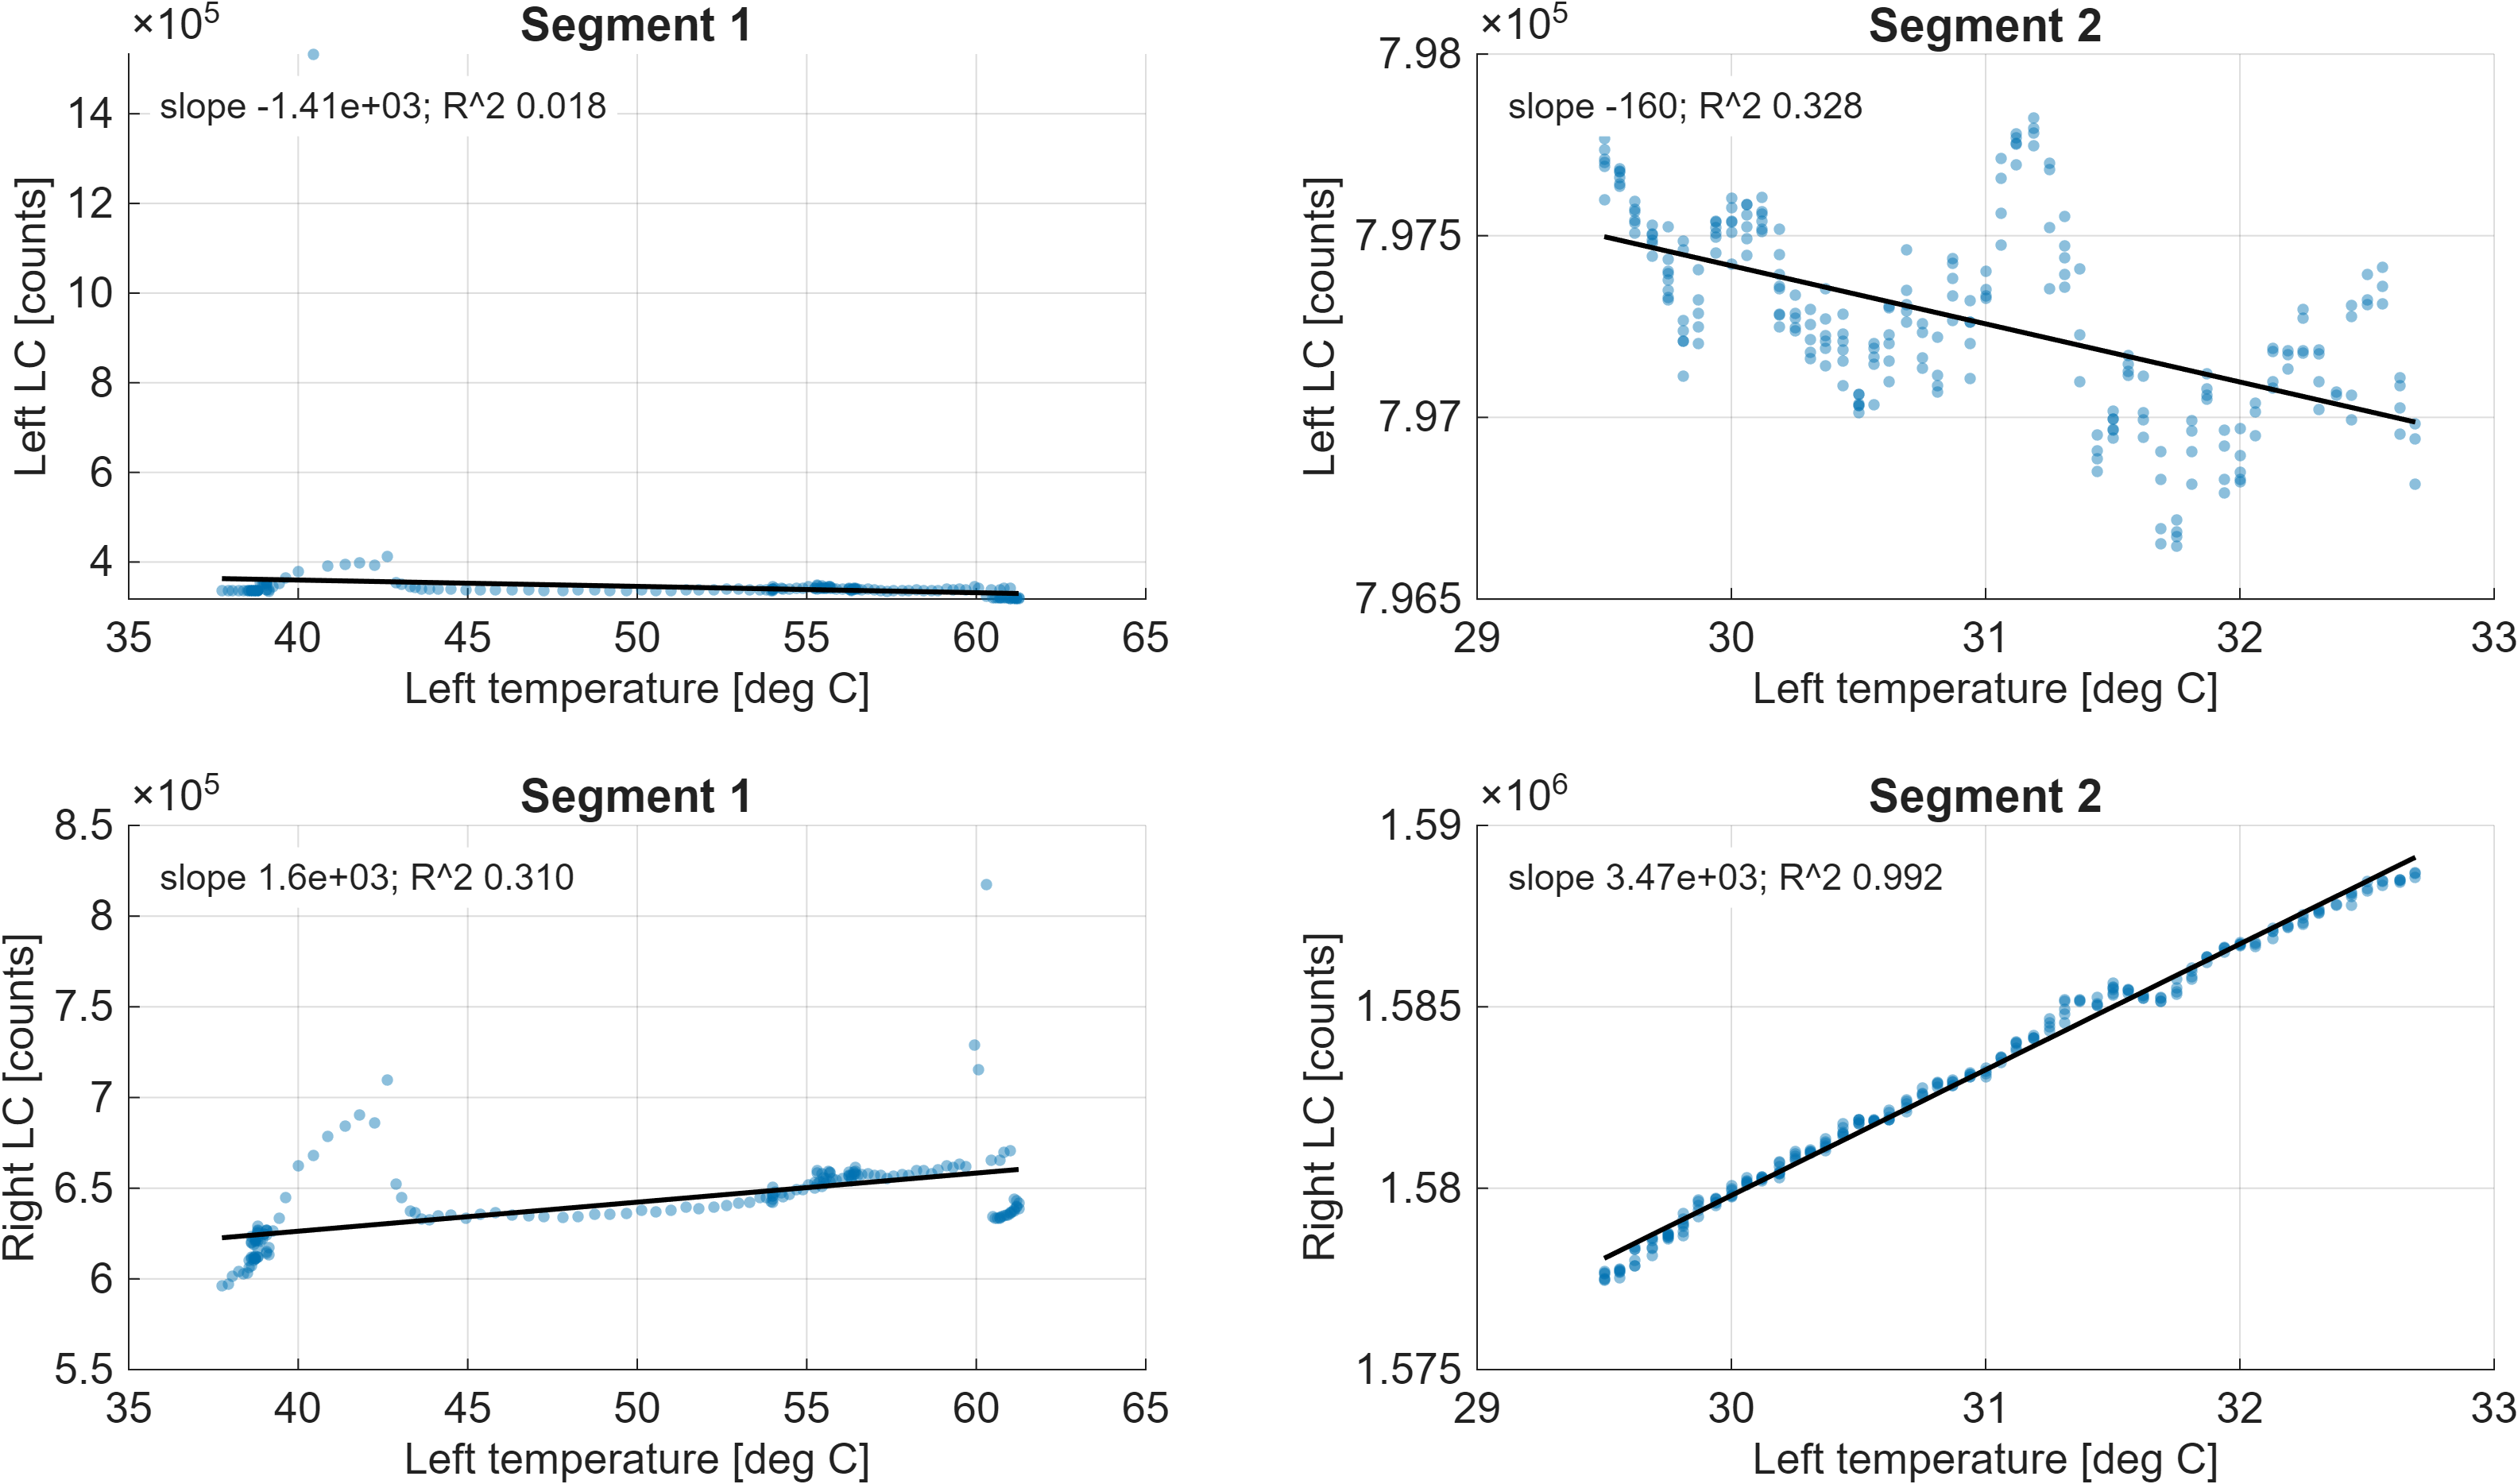
\includegraphics[width=\textwidth,height=0.37\textheight,keepaspectratio]{figures/F23_thermal_loadcell_temperature.png}
\caption{Load-cell versus left temperature using occupied one-second bins in each thermal segment.}\label{fig:F23}
\end{figure}
The right load cell has a much more coherent temperature association during cooling: slope 3465.6 counts/deg C with R-squared 0.992, compared with 1602.6 and 0.310 during heating. The left channel is less consistent: its heating slope is -1411.7 counts/deg C but R-squared is only 0.018; the cooling values are -160.0 and 0.328. The conspicuous heating-segment excursions weaken a single straight-line description even after median binning. Differential sensor electronics, mounting expansion and changing mechanical preload are plausible contributors, but the channels cannot be calibrated thermally from these associations alone. In particular, the strong cooling fit may arise because both output and temperature drift with elapsed time. Independent controlled cycles and fixed loading are needed to distinguish temperature effects from shared temporal trends.\par

\renewcommand{\thefigure}{F24}
\begin{figure}[H]\centering
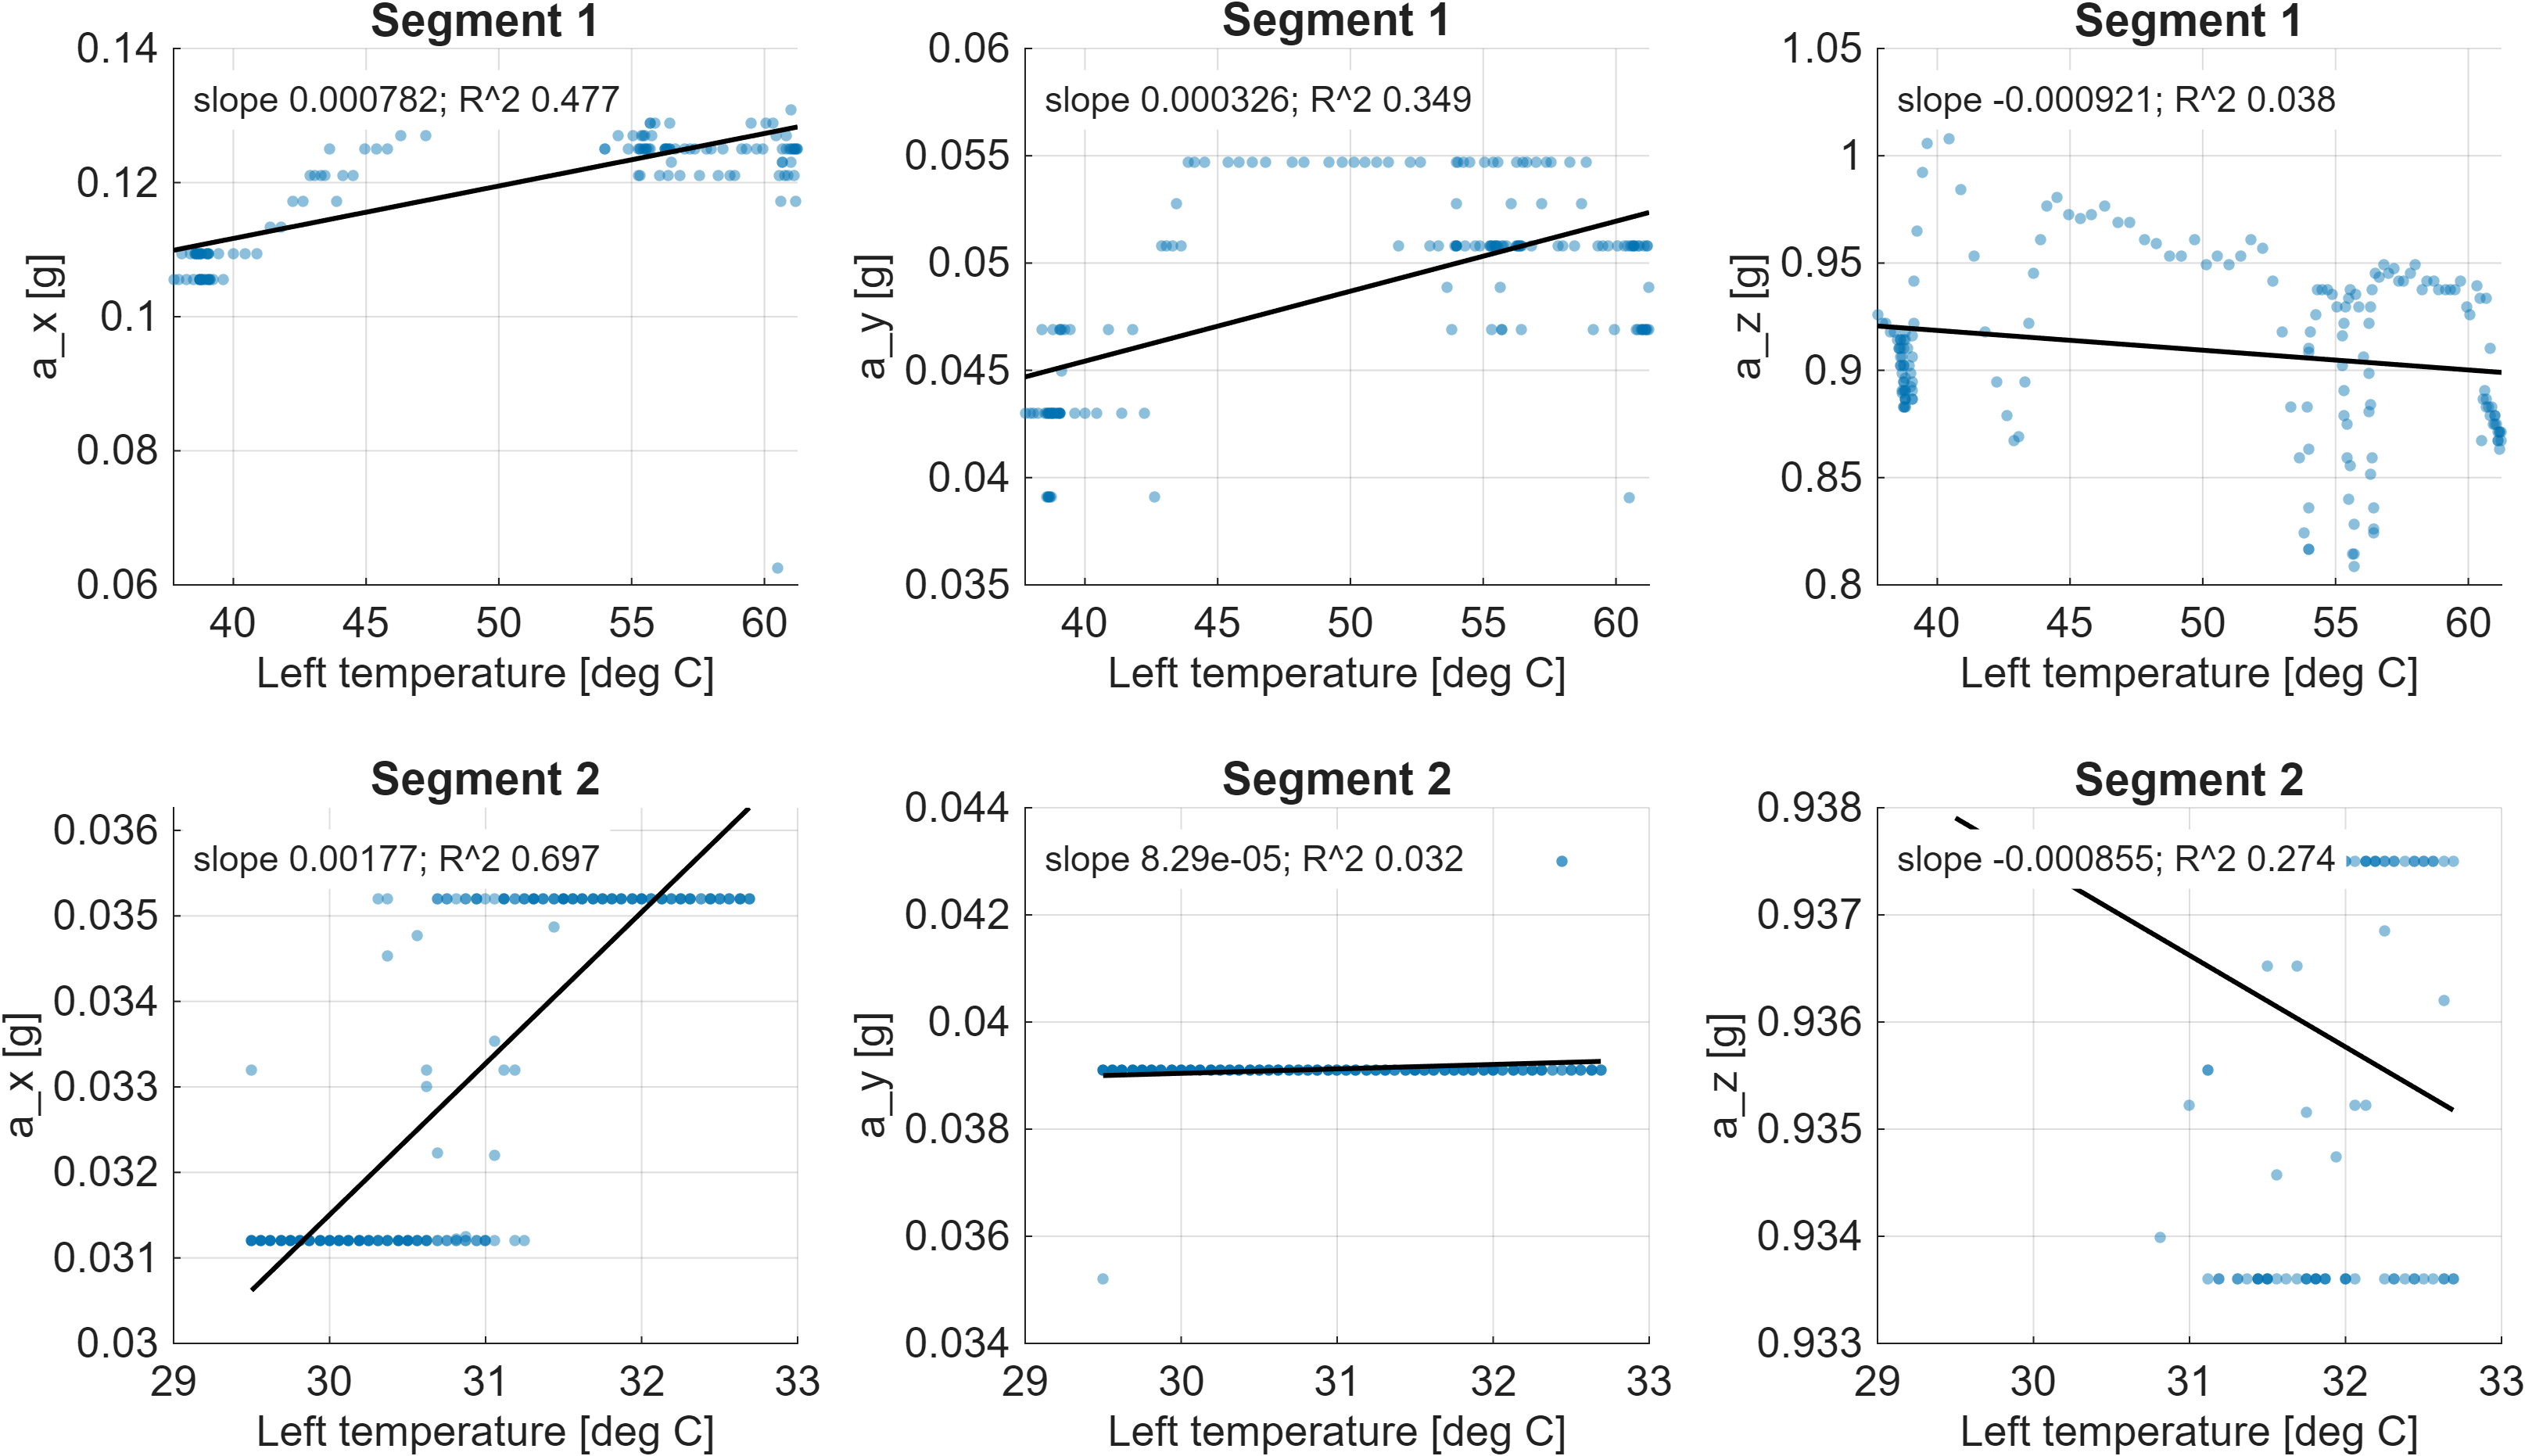
\includegraphics[width=\textwidth,height=0.37\textheight,keepaspectratio]{figures/F24_thermal_accel_temperature.png}
\caption{Acceleration offsets versus temperature in separate thermal segments.}\label{fig:F24}
\end{figure}
Acceleration-level associations are axis dependent and do not behave as a single thermal offset. The x slope is positive in both segments: 0.000782 and 0.001770 g/deg C, with R-squared 0.477 and 0.697. The z slopes are negative, -0.000921 and -0.000855 g/deg C, but heating explains little of the z variation (R-squared 0.038). Cooling y is almost unrelated to left temperature (R-squared 0.032). Quantized bands and large heating-segment excursions further limit a smooth linear model. Electronics drift is plausible, but these levels also contain gravity projection, orientation and mechanical motion; a small tilt can mimic an acceleration offset. Environmental compensation should therefore retain axis-specific hypotheses and test them on controlled independent sessions, rather than subtracting these slopes directly from dynamic data.\par

\renewcommand{\thefigure}{F25}
\begin{figure}[H]\centering
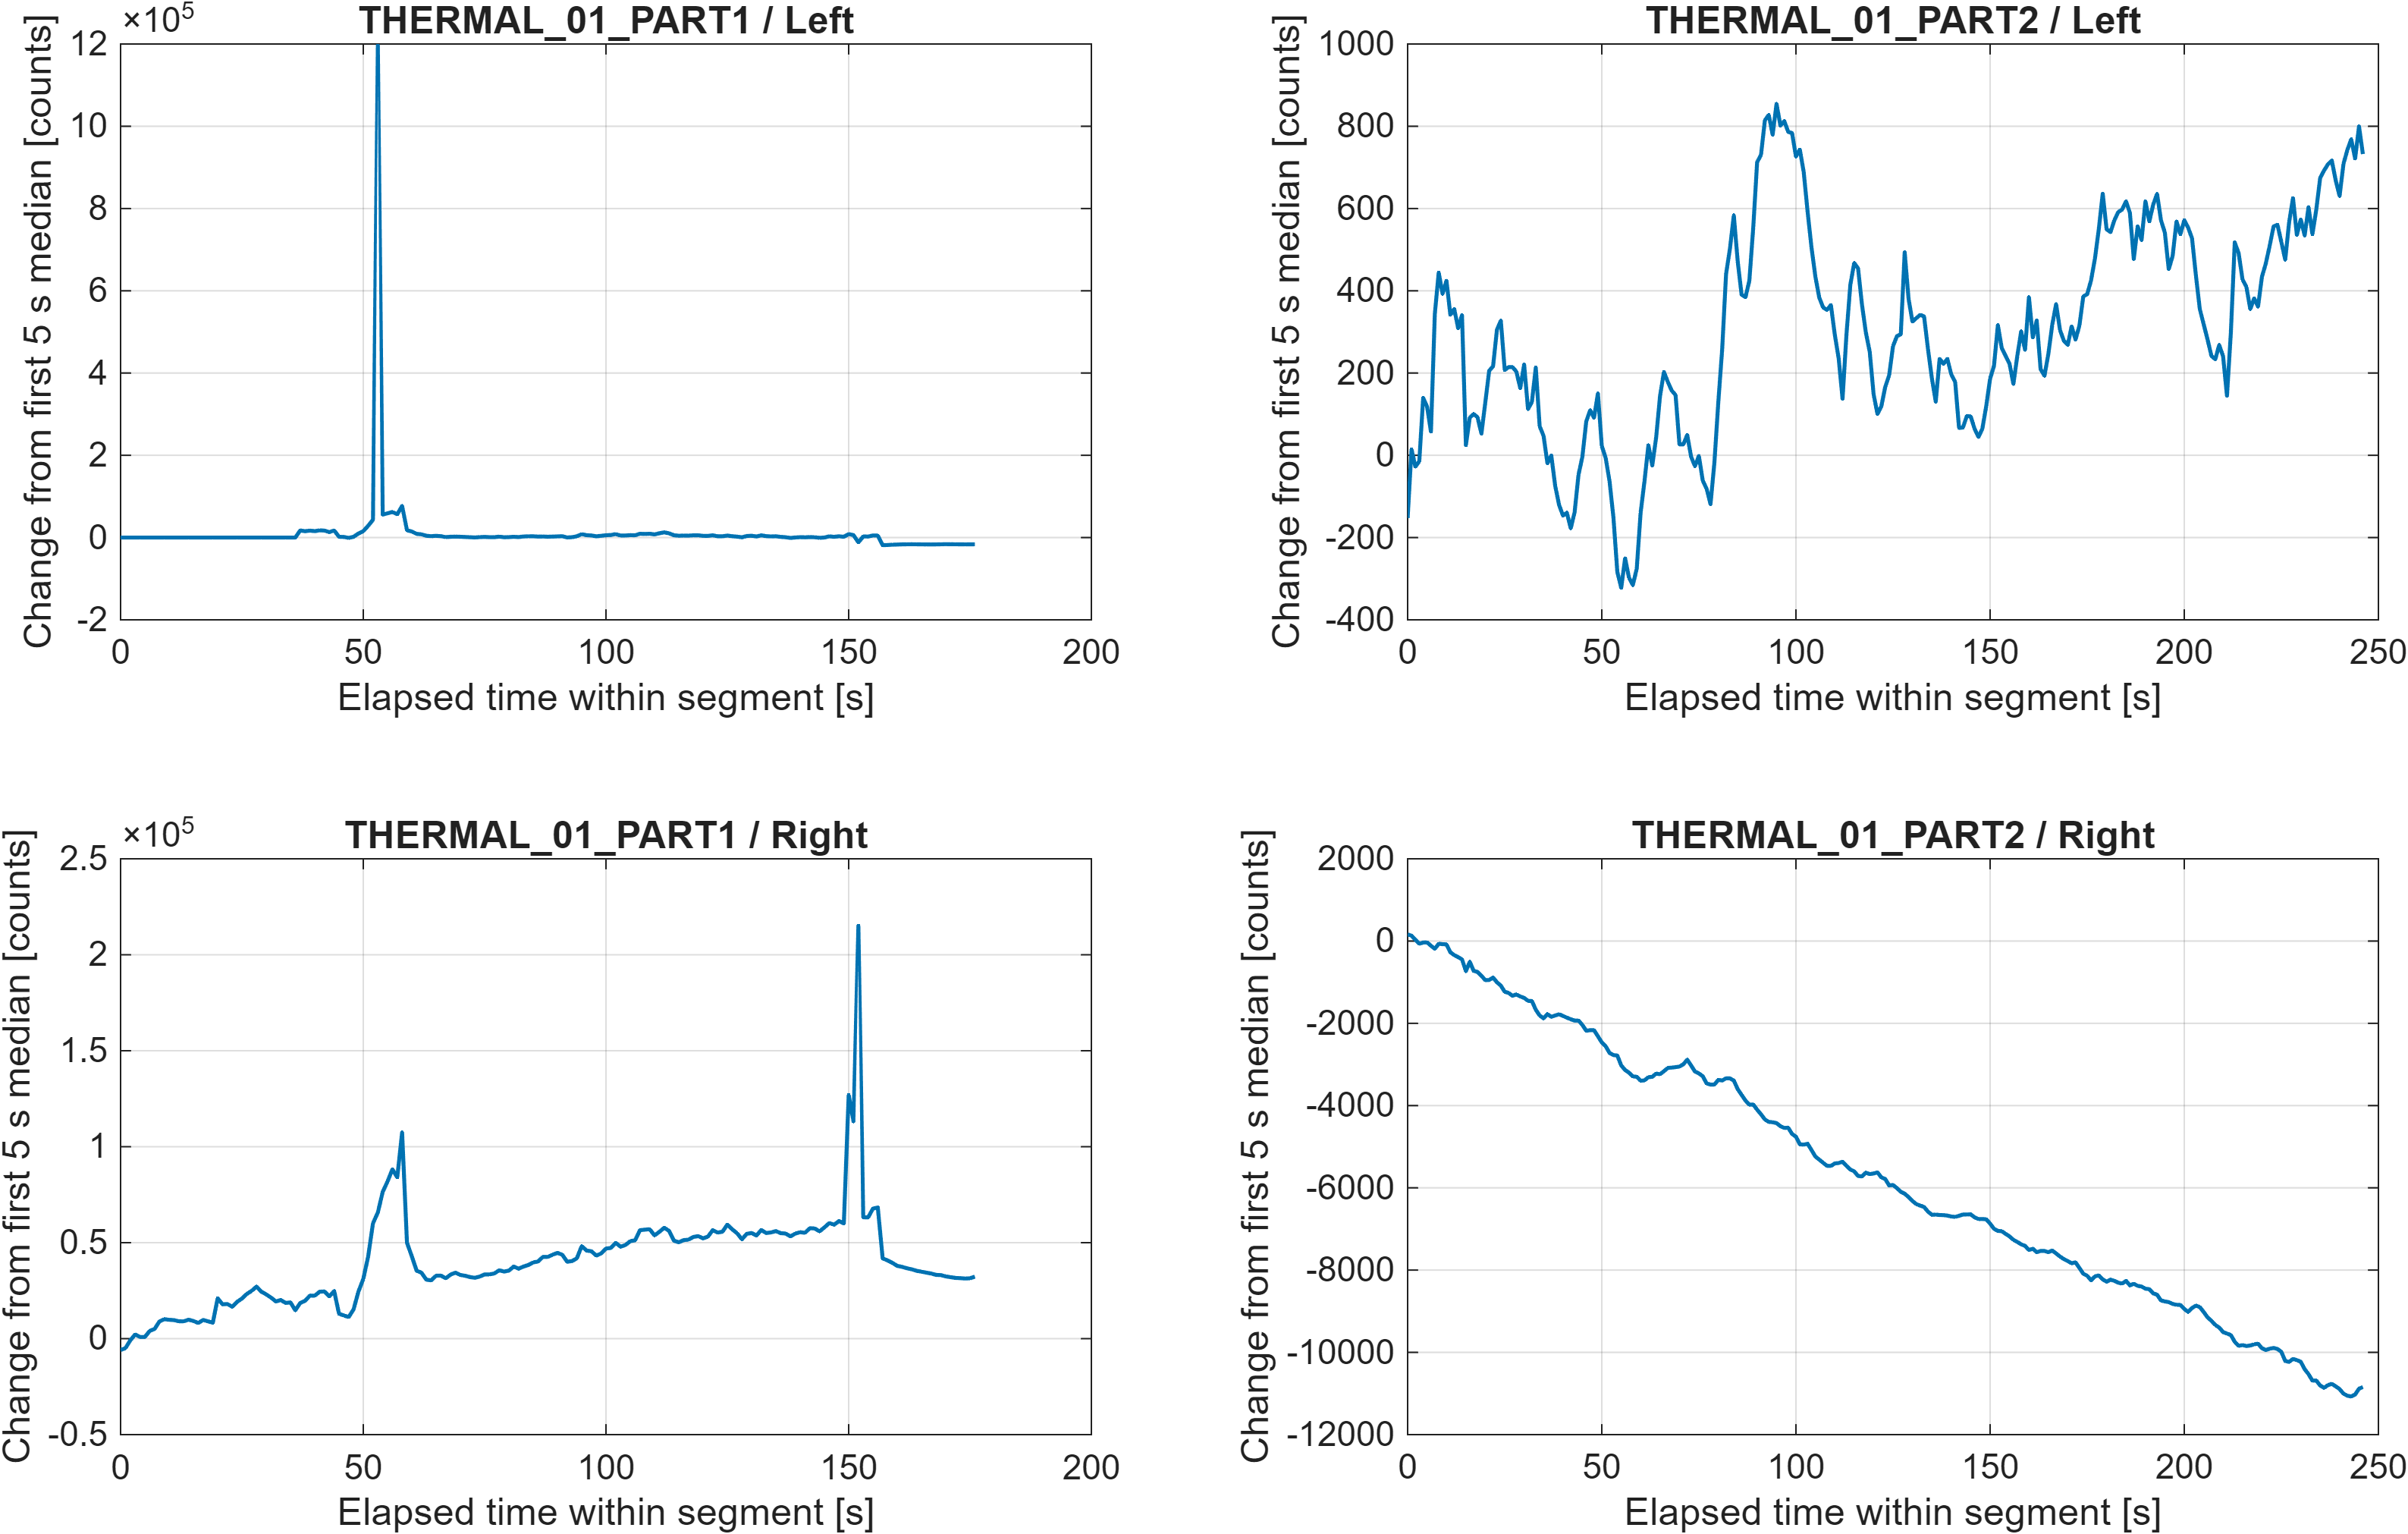
\includegraphics[width=\textwidth,height=0.37\textheight,keepaspectratio]{figures/F25_thermal_elapsed_drift.png}
\caption{Within-segment load-cell changes relative to the first five seconds of occupied one-second bins.}\label{fig:F25}
\end{figure}
The elapsed-time view distinguishes persistent drift from transient excursions. Heating-segment final-minus-initial median changes are -16395 counts on the left and +31579 on the right; cooling changes are +738 and -11014 counts. The cooling right channel decreases relatively smoothly, while the left drifts weakly upward despite cooling, consistent with the opposite fitted slope signs. Heating instead contains large short-lived departures superimposed on the endpoint changes. Thermally induced preload changes or sensor drift are possible explanations, but the excursions also require acquisition and handling review. Separate segment baselines prevent the large inter-segment offset from being misrepresented as observed continuous drift. Endpoint summaries are therefore useful for comparing within-segment behavior, but cannot partition thermal, mechanical and instrumentation contributions.\par

\renewcommand{\thefigure}{F26}
\begin{figure}[H]\centering
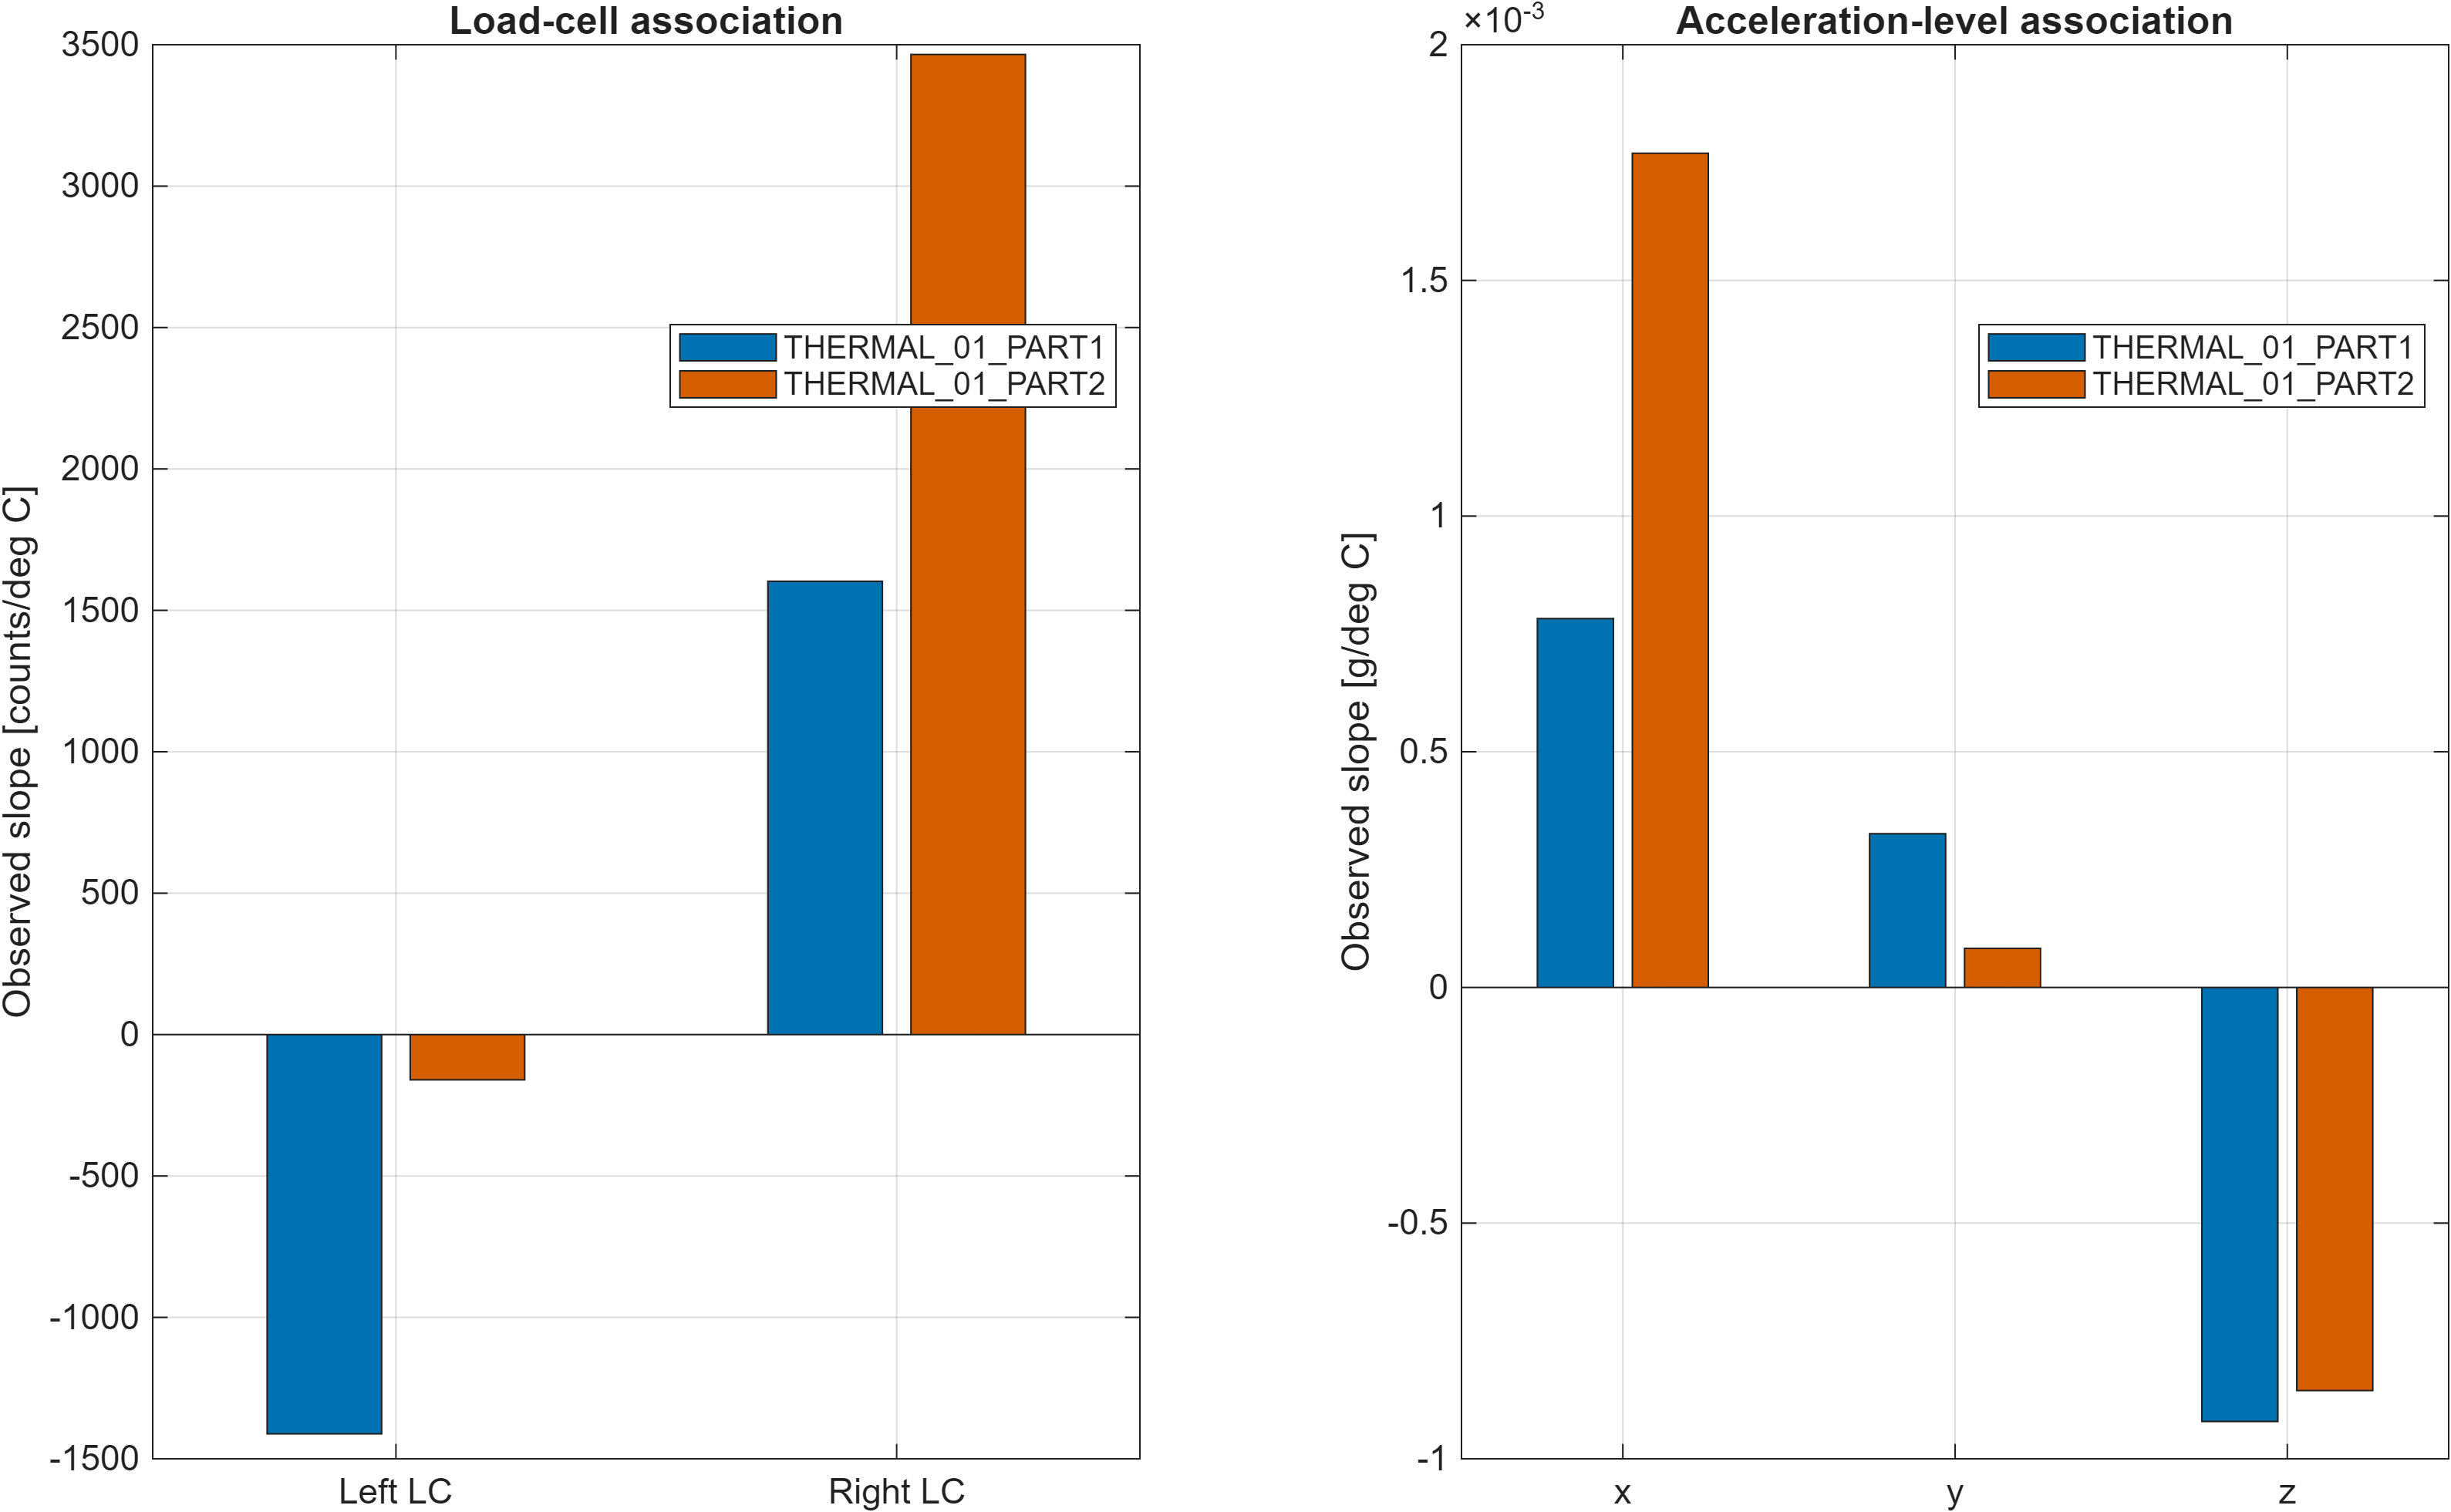
\includegraphics[width=\textwidth,height=0.37\textheight,keepaspectratio]{figures/F26_thermal_sensitivity_summary.png}
\caption{Comparison of fitted thermal associations by sensor and segment.}\label{fig:F26}
\end{figure}
The fitted sensitivity comparison highlights nontransferability between the two segments. The right-cell cooling slope is 2.16 times its heating slope, with R-squared improving from 0.310 to 0.992. The absolute left-cell heating slope is 8.82 times its cooling slope, yet its heating R-squared is only 0.018; a large slope therefore does not necessarily indicate a reliable temperature relationship. Acceleration axes also differ in sign and fit quality. These contrasts suggest that a single coefficient per sensor would confound operating state, temperature range and elapsed-time effects. The strongest fit is a useful hypothesis for a controlled follow-up experiment, not a validated correction. Compensation should be evaluated by its prediction error on independent fixed-load thermal cycles, with sensor-specific uncertainty and residual drift reported.\par

\Needspace{5\baselineskip}
\section{Wind and Impact Disturbances}
Wind and impact recordings are summarized individually because exact event timing, forcing magnitude and wind speed are not supplied. Two wind recordings also have PWM 192, so motor operation is a confounder. No dedicated undisturbed reference is assumed. Impact-recording envelopes are aligned to the largest observed dynamic residual, which is a computed feature rather than a verified impact trigger. Pre- and post-feature windows are descriptive and are not labeled as confirmed baseline and settling intervals.

\renewcommand{\thefigure}{F27}
\begin{figure}[H]\centering
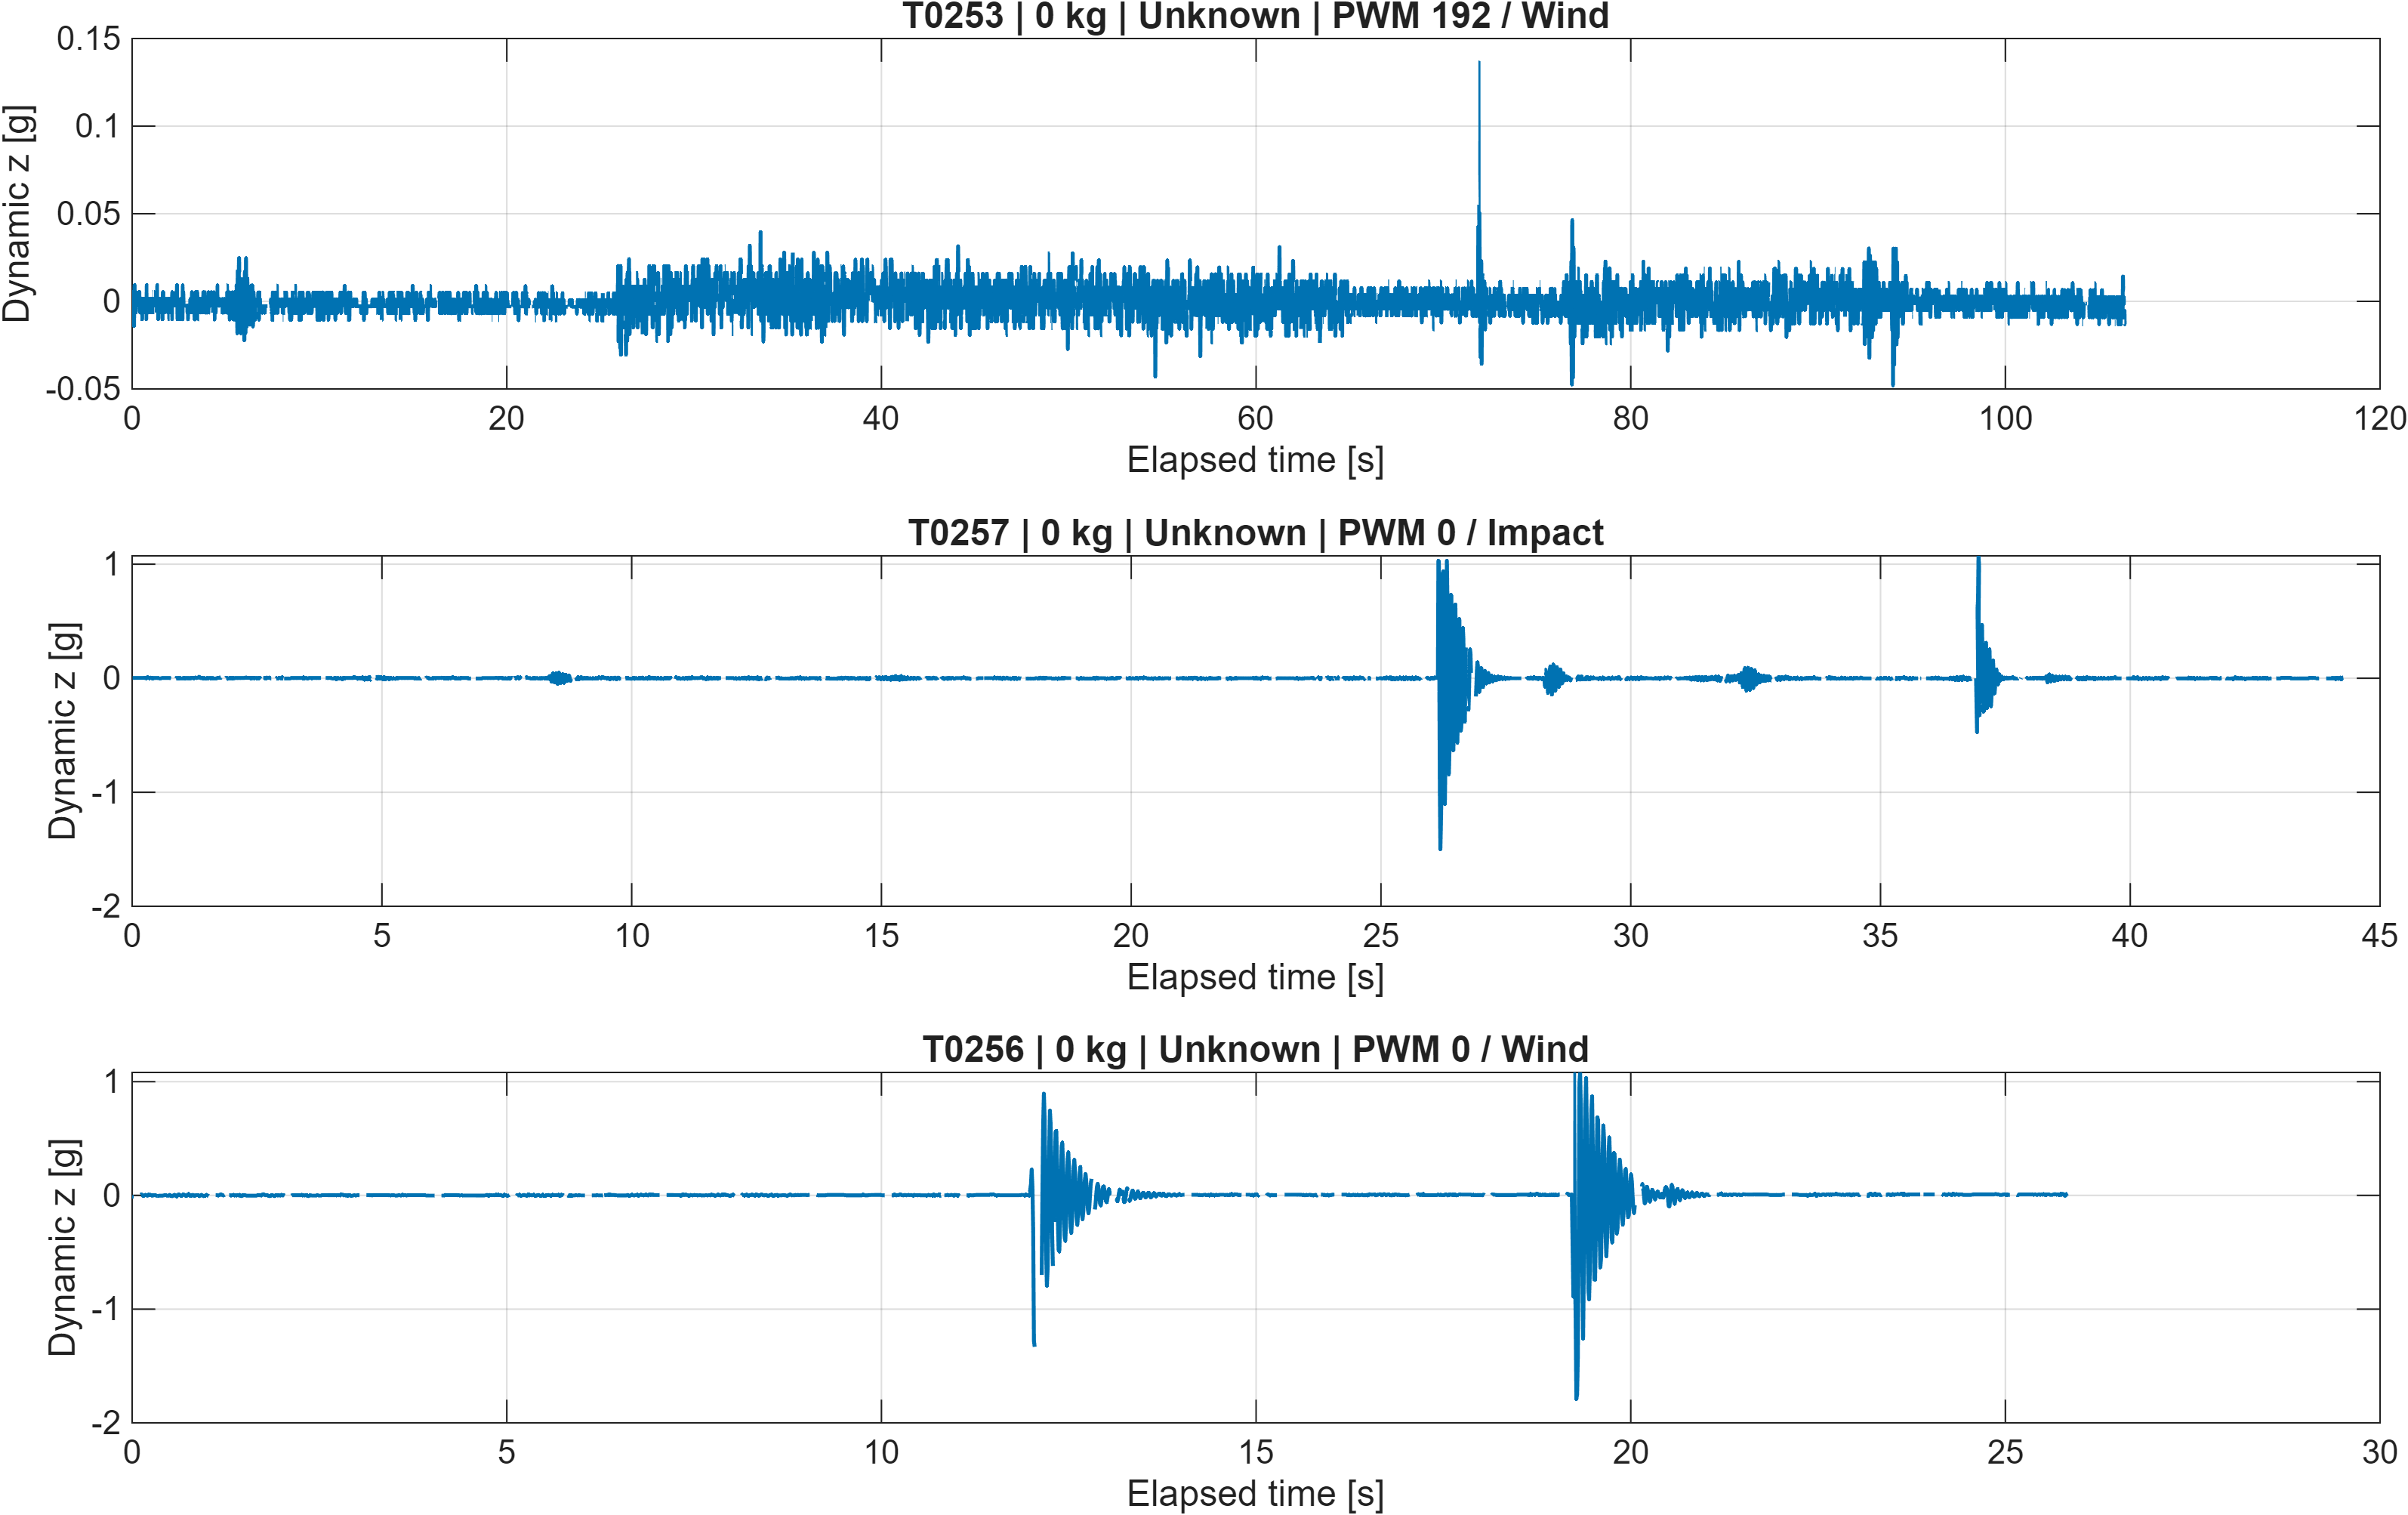
\includegraphics[width=\textwidth,height=0.37\textheight,keepaspectratio]{figures/F27_disturbance_transients.png}
\caption{Representative cleaned disturbance recordings with timestamp-linear trends removed.}\label{fig:F27}
\end{figure}
The representative no-motor wind record reaches 1.790 g, compared with 1.500 g in the representative impact record and 0.136 g in the PWM 192 wind record. The larger wind-labelled transient is therefore not consistent with ranking disturbance severity by label alone. The no-motor wind and impact traces contain localized bursts followed by visibly smaller oscillations, whereas the motor-assisted wind trace has a more persistent low-amplitude background. This is compatible with different forcing histories and subsequent decay, but labels do not specify the input waveform. Peaks may also be affected by upstream cleaning and acquisition gaps. Without synchronized impact timing or measured wind forcing, no reliable decay constant, damping ratio or causal wind-versus-impact comparison can be extracted.\par

\renewcommand{\thefigure}{F28}
\begin{figure}[H]\centering
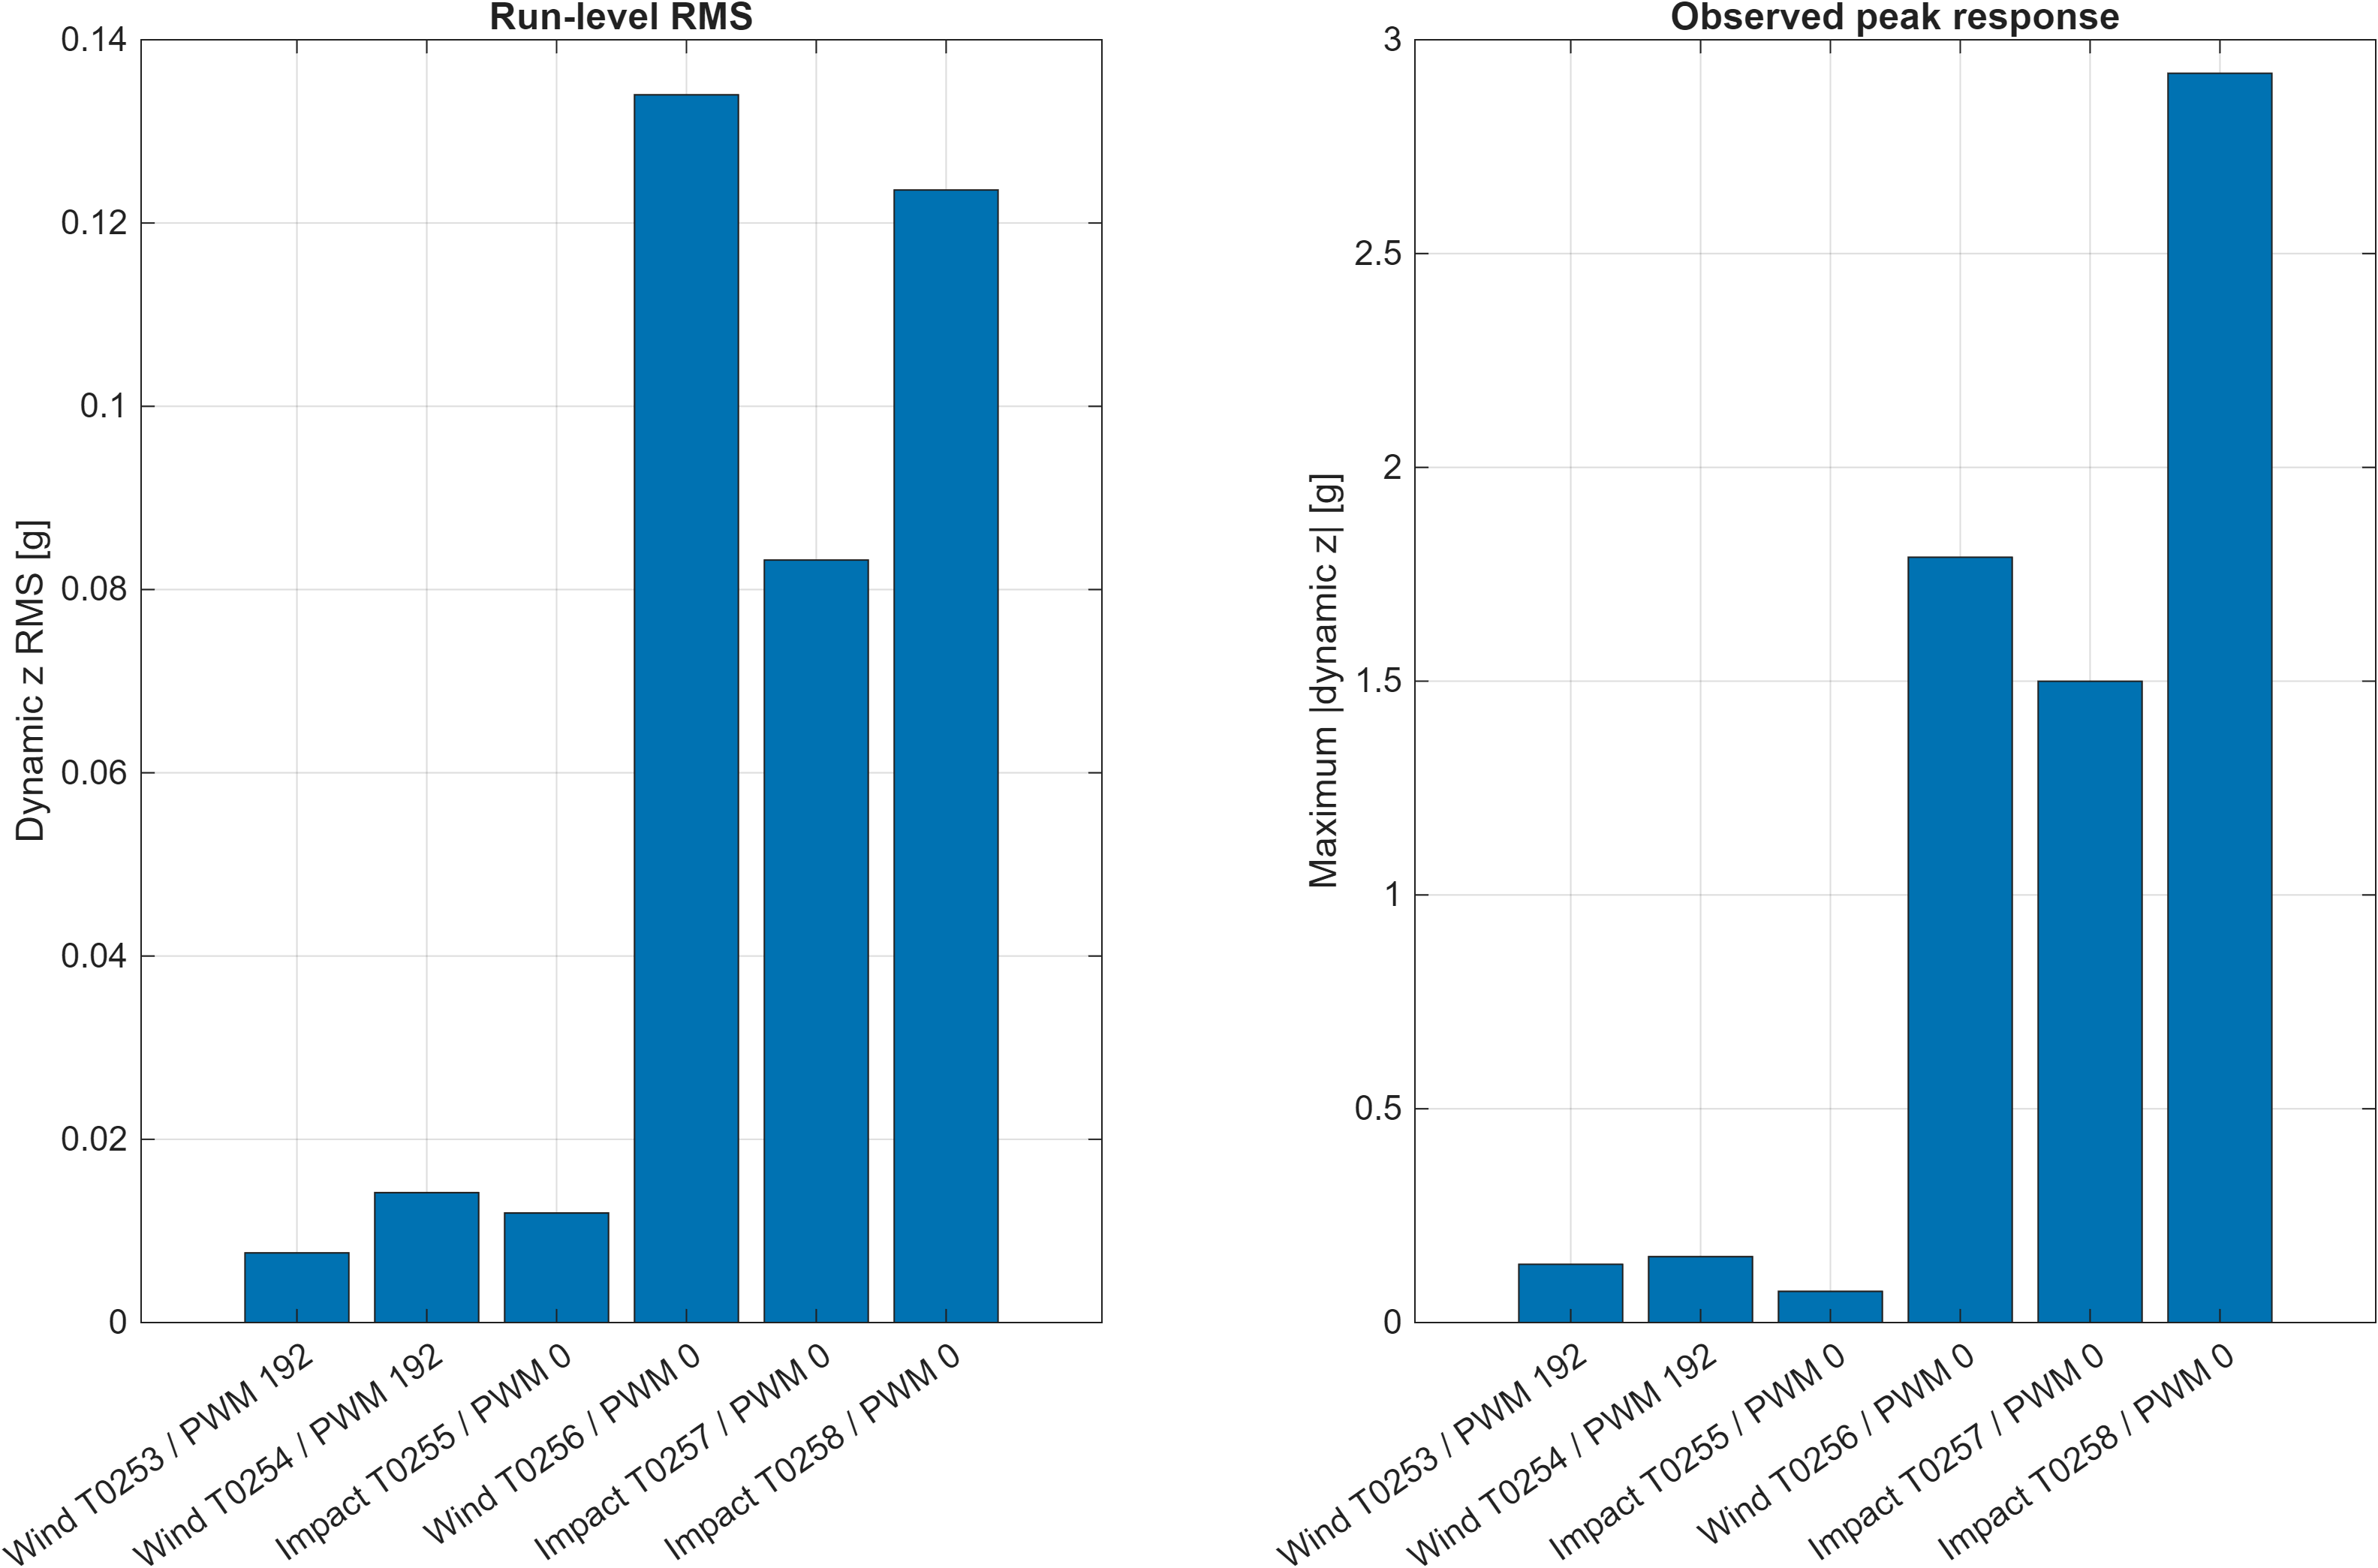
\includegraphics[width=\textwidth,height=0.37\textheight,keepaspectratio]{figures/F28_disturbance_metrics.png}
\caption{Disturbance RMS and observed peak by run, with motor commands identified.}\label{fig:F28}
\end{figure}
Impact recordings are highly heterogeneous: observed z peaks span 0.073--2.922 g, a factor of 40.0. The strongest impact, T0258, has RMS 0.1236 g, while the no-motor wind recording T0256 has RMS 0.1340 g and a smaller peak of 1.790 g. Thus peak and RMS emphasize different features of the excitation: concentrated impulses versus more sustained or repeated motion. The two PWM 192 wind records have much lower RMS, 0.0076 and 0.0142 g, despite motor operation. Unknown wind intensity, handling and event timing prevent interpreting this as motor-induced suppression. These results argue for recording forcing and event metadata before training a disturbance classifier or response model; current labels are insufficient proxies for excitation magnitude or duration.\par

\renewcommand{\thefigure}{F29}
\begin{figure}[H]\centering
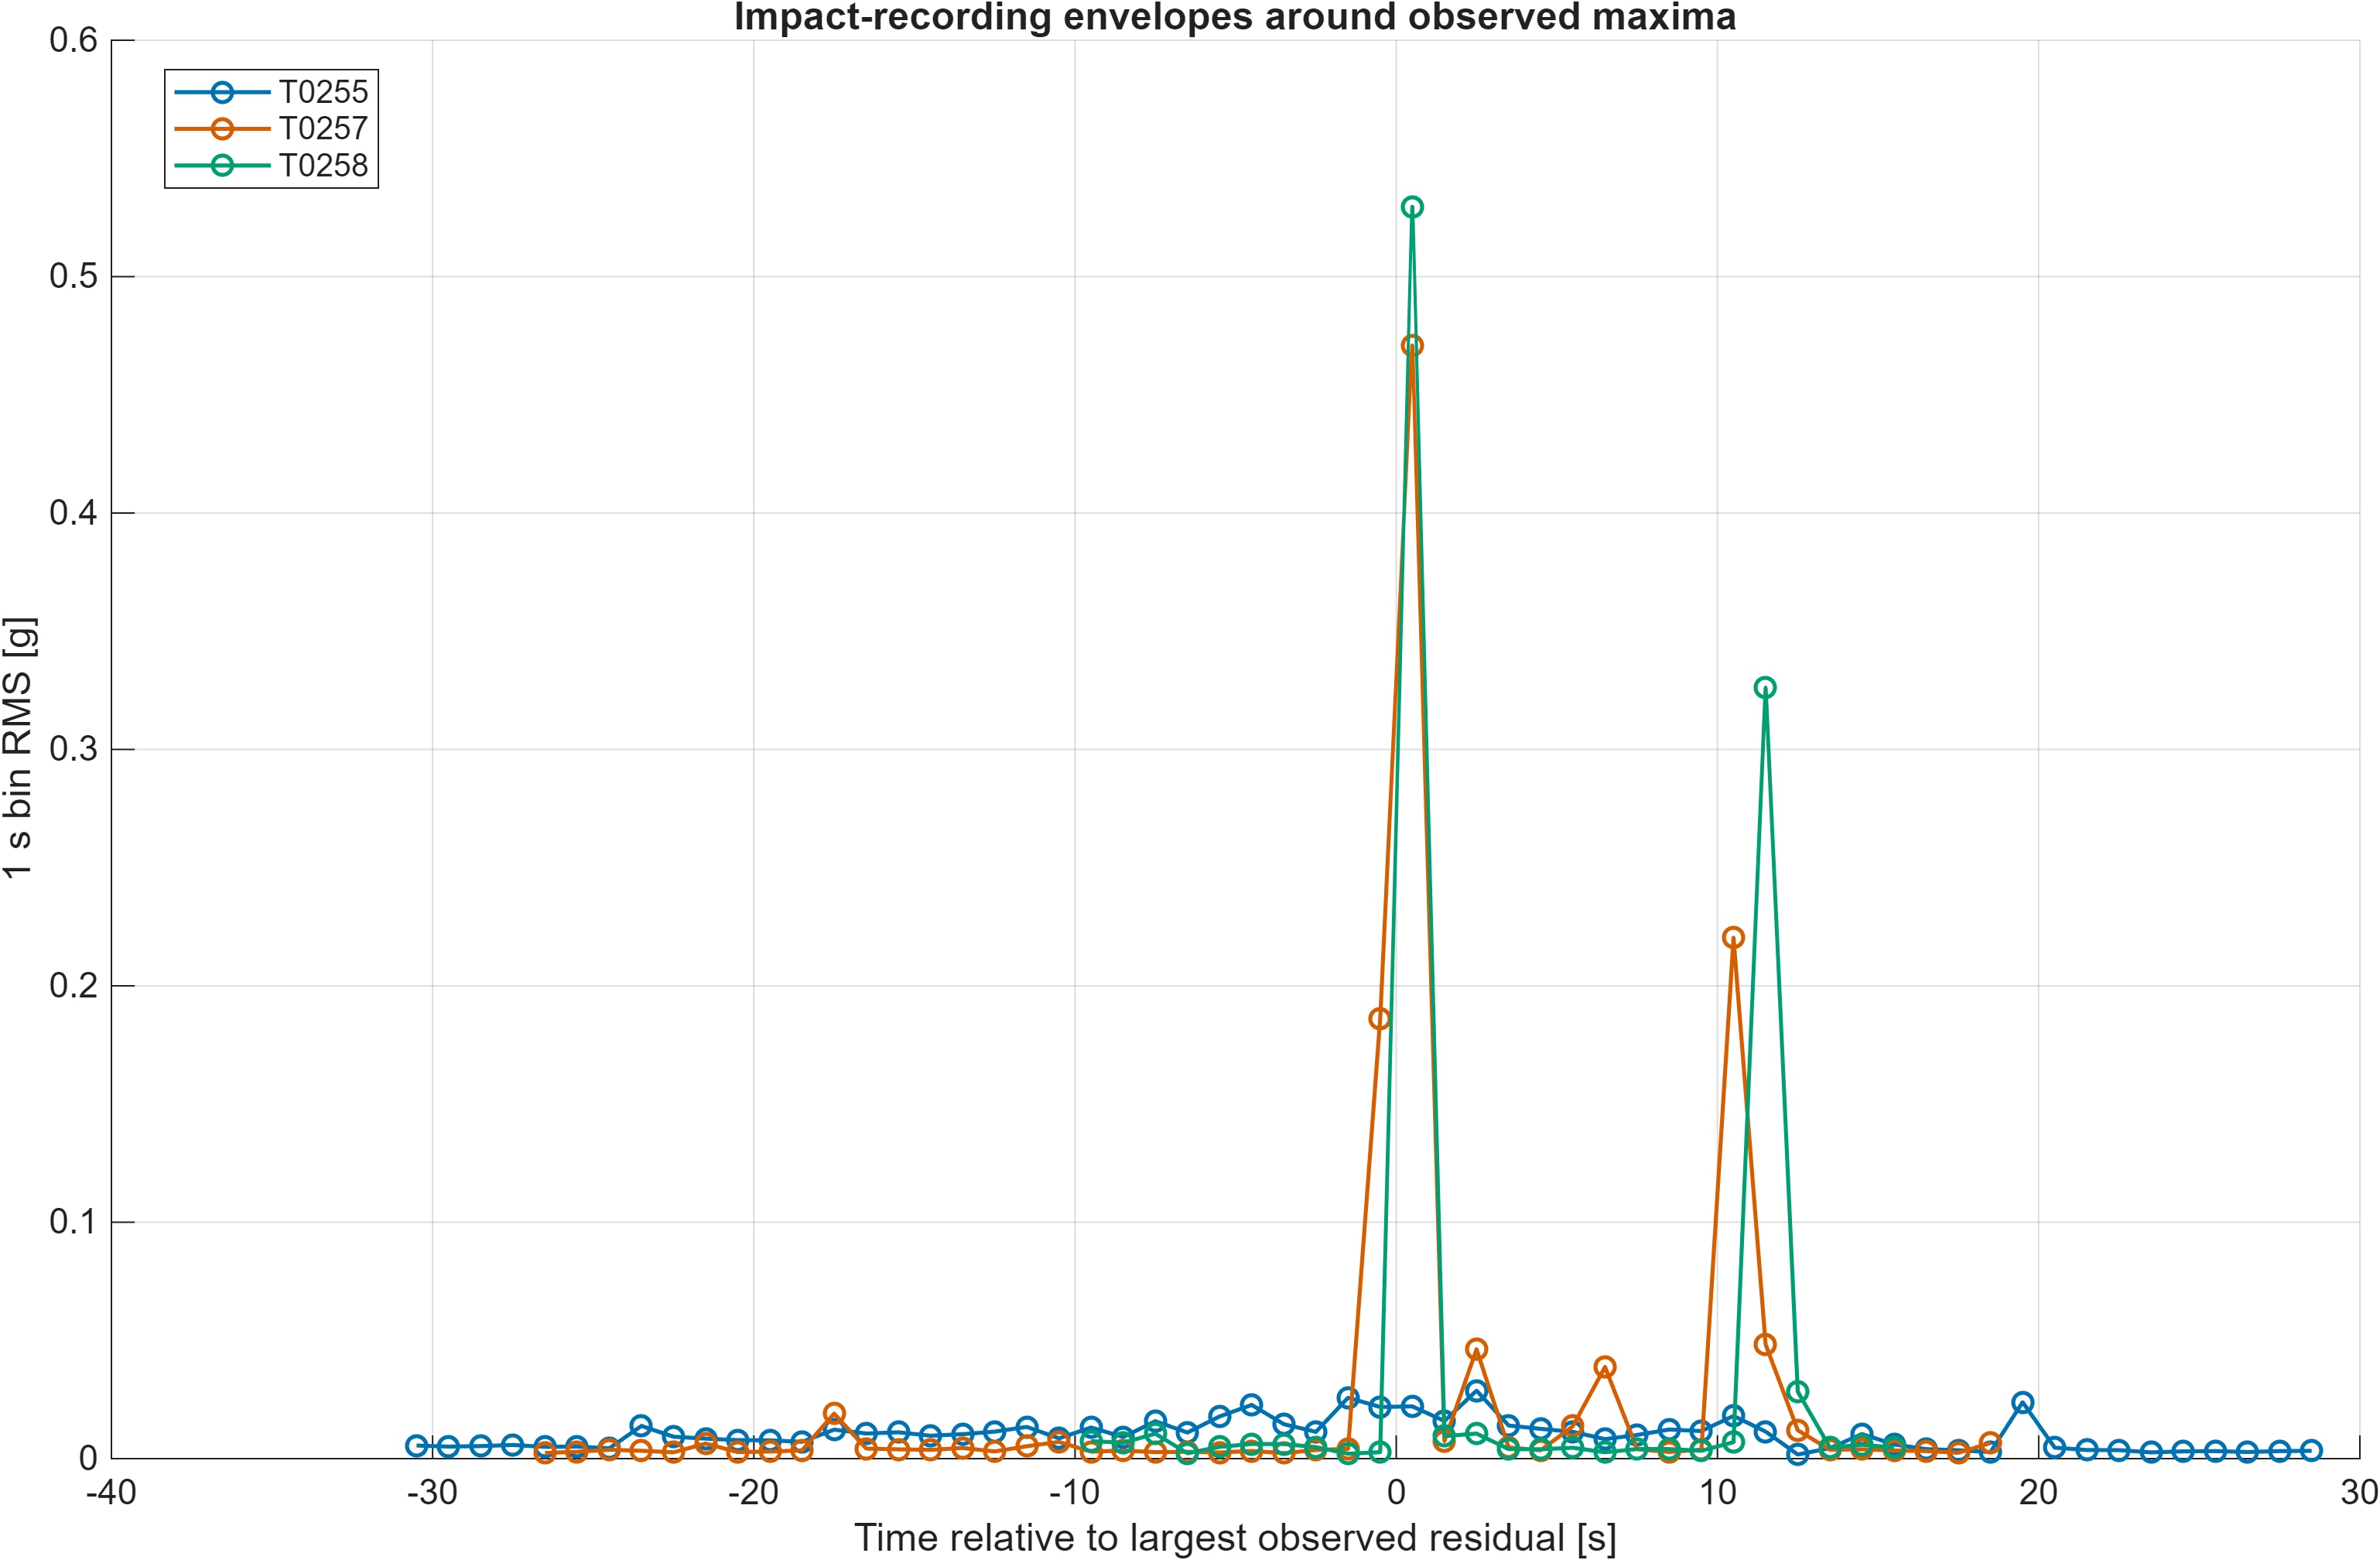
\includegraphics[width=\textwidth,height=0.37\textheight,keepaspectratio]{figures/F29_impact_envelopes.png}
\caption{One-second RMS envelopes aligned to each recording's largest observed residual.}\label{fig:F29}
\end{figure}
The largest-event neighborhoods concentrate 11.3, 81.6 and 71.3 percent of squared residual samples within plus/minus one second in T0255, T0257 and T0258, respectively. The stronger impact records are therefore dominated by brief bursts rather than uniform vibration. Their envelopes fall after the largest burst, but secondary peaks and nonzero residual motion prevent a unique free-decay interpretation. For T0258, the median one-second RMS is 0.00551 g in the pre-feature window and 0.00678 g afterward; the post-window is not a demonstrated return to baseline. Alignment uses the largest measured residual, not a recorded trigger. Missing samples, upstream filtering and unknown repeated forcing preclude reliable damping estimation; the apparent envelope is descriptive evidence for better event-synchronized tests.\par

\Needspace{5\baselineskip}
\section{Comparative Experimental Findings}
The summary figures emphasize within-batch dynamic response coverage, the recorded experimental design, and limitations that affect interpretation. Means of run metrics have equal recording weights. Coverage plots combine metadata only and do not imply that responses from different acquisition batches are interchangeable.

\renewcommand{\thefigure}{F30}
\begin{figure}[H]\centering
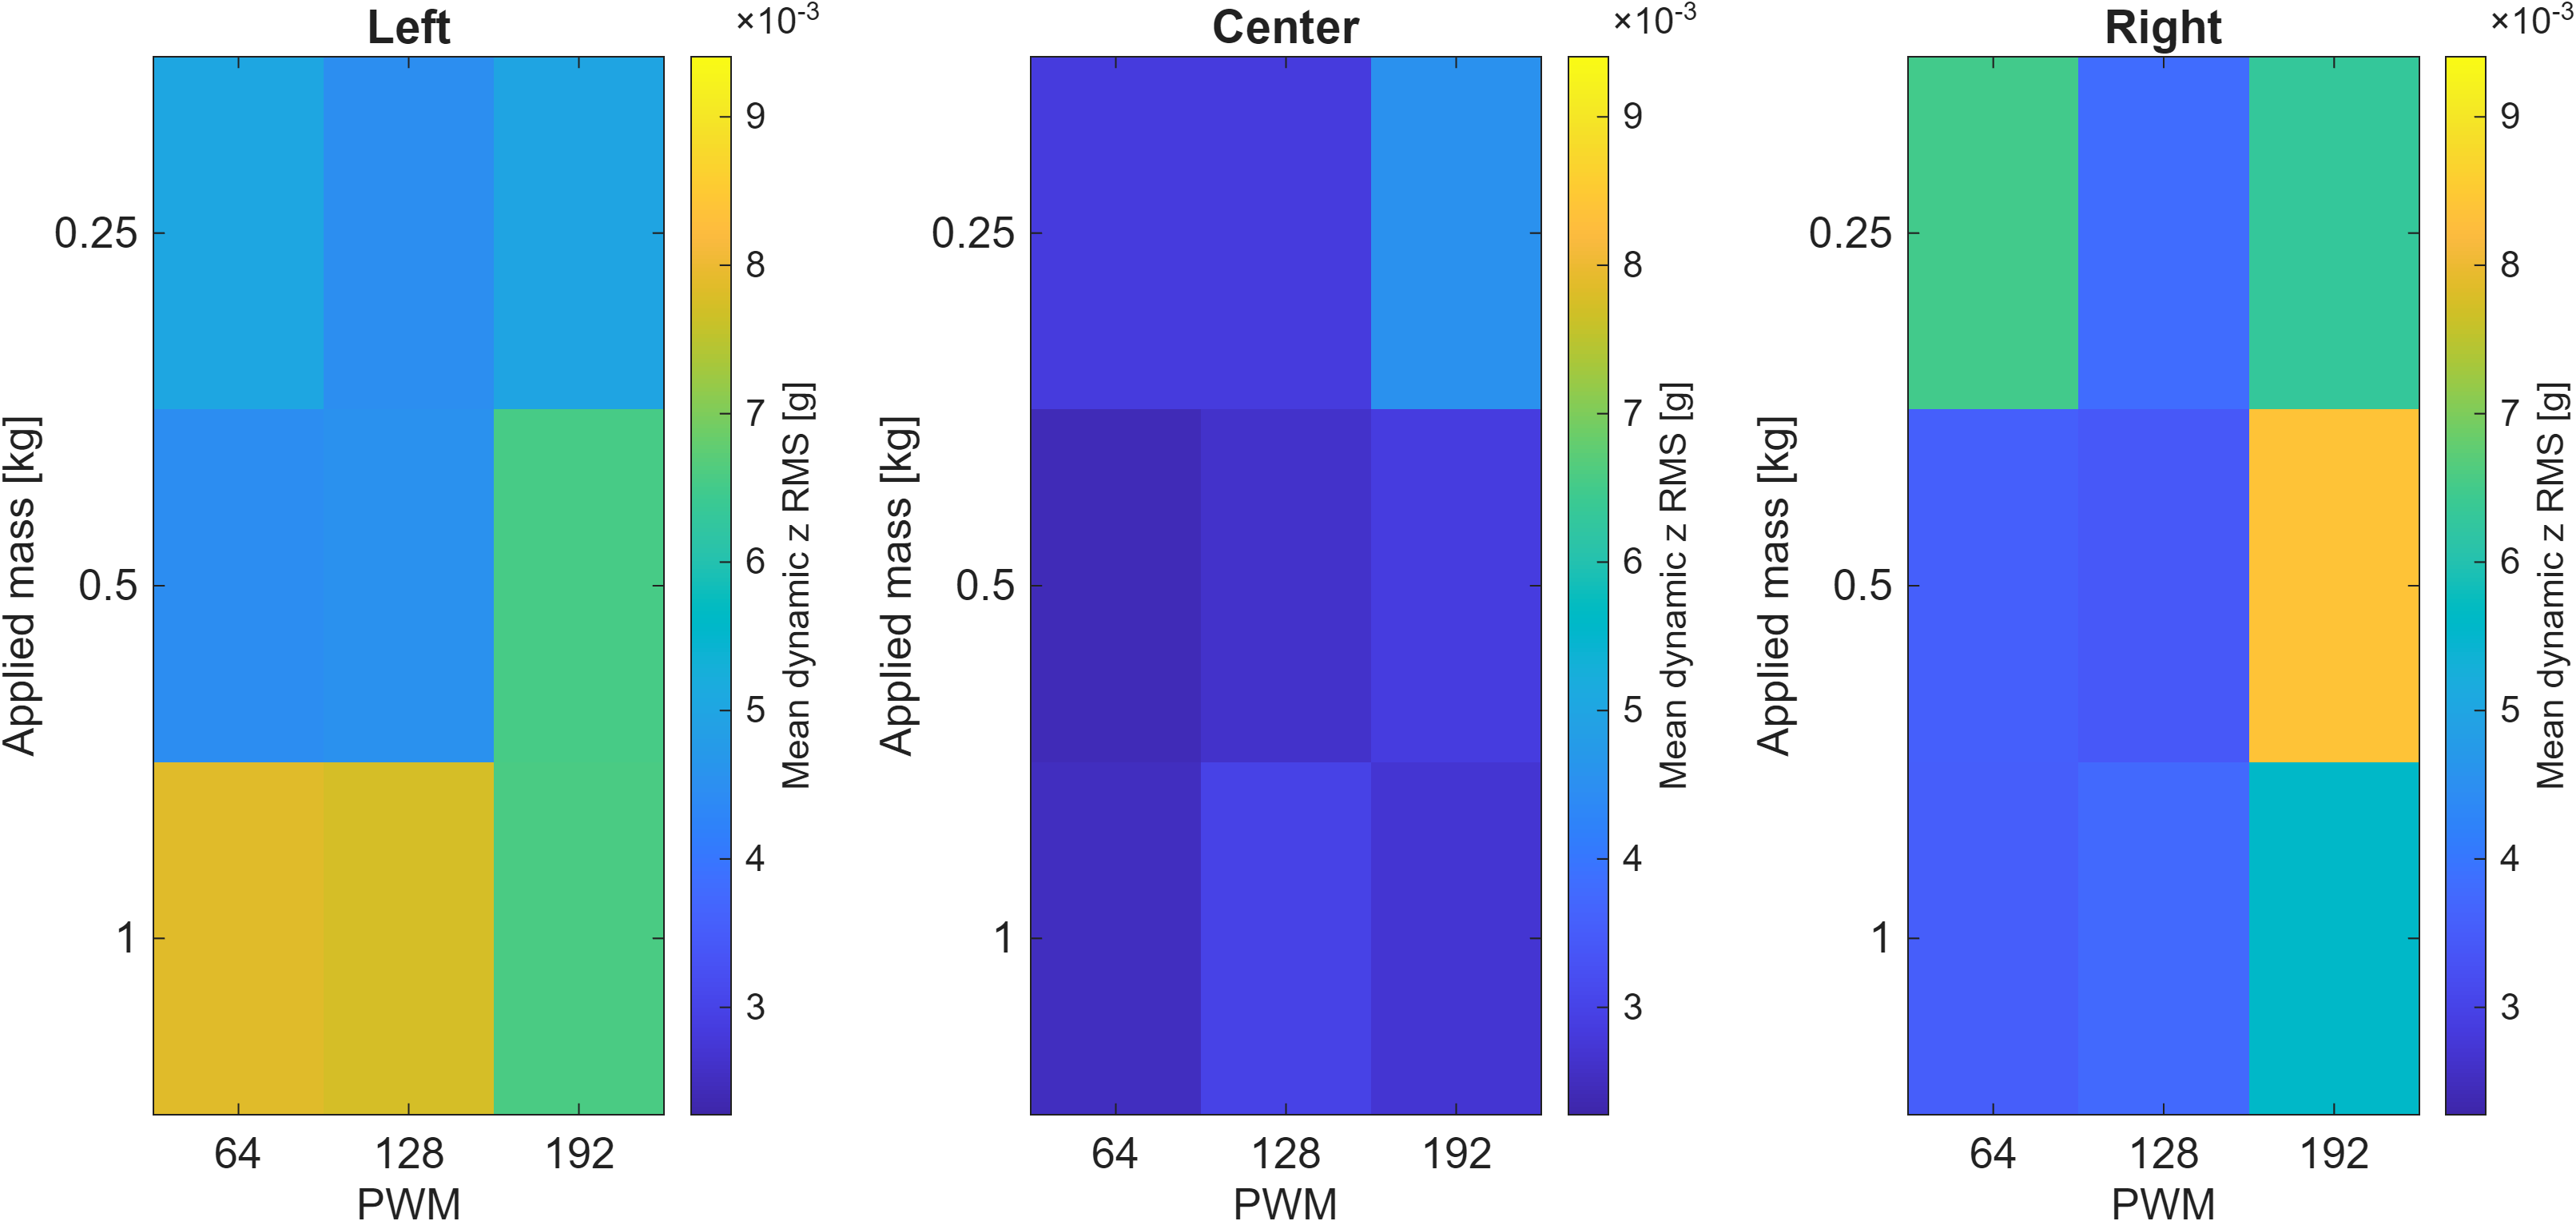
\includegraphics[width=\textwidth,height=0.37\textheight,keepaspectratio]{figures/F30_combined_response_map.png}
\caption{Same-batch map of mean dynamic z RMS [g] across mass, PWM and position.}\label{fig:F30}
\end{figure}
The same-batch response map is structured primarily by position rather than a uniformly increasing mass or PWM scale. The lowest condition mean is 0.00244 g at 0.50 kg, normalized position 0.50, PWM 64; the highest is 0.00839 g at 0.50 kg, position 0.75, PWM 192, a factor of 3.44. Center loading remains lower than both edges across the matched grid, while edge responses vary nonmonotonically with mass. This supports retaining interactions among operating variables in future identification instead of fitting independent scalar corrections. However, the grid contains only a few repetitions per cell and one singleton. Apparent spatial structure is a hypothesis about this setup, not a validated response surface or evidence of a particular mode shape.\par

\renewcommand{\thefigure}{F31}
\begin{figure}[H]\centering
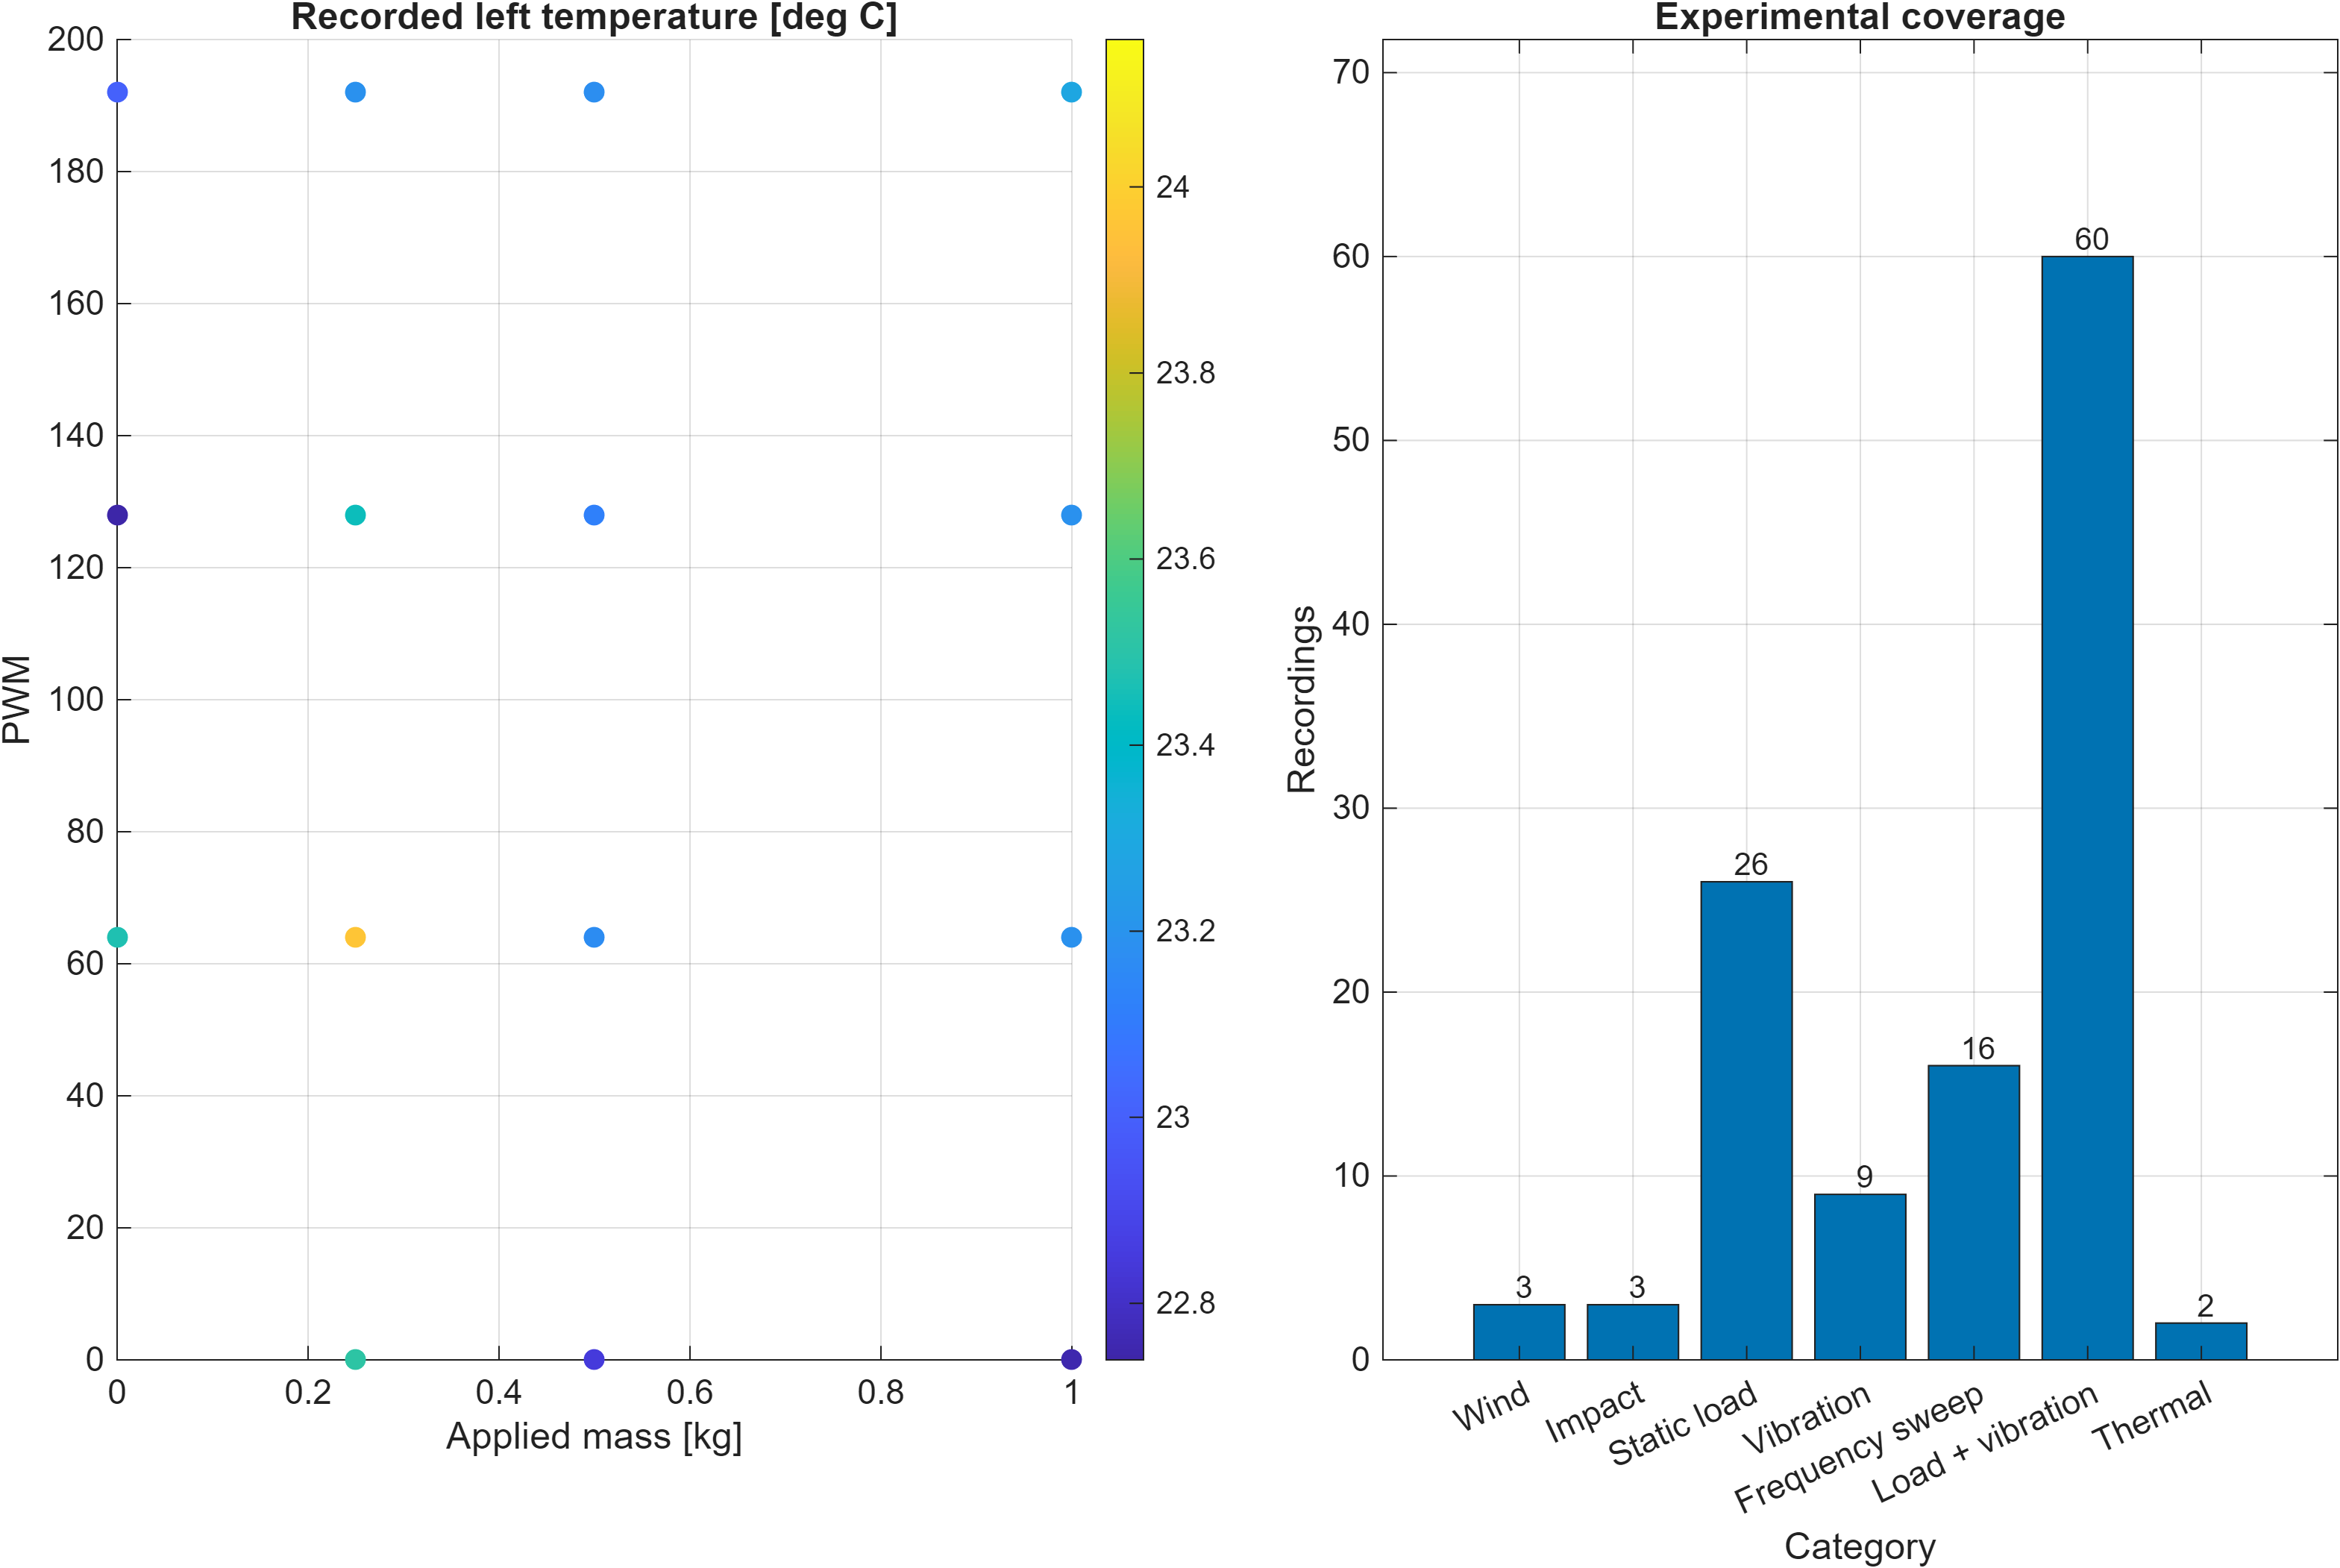
\includegraphics[width=\textwidth,height=0.37\textheight,keepaspectratio]{figures/F31_coverage_summary.png}
\caption{Coverage of load, motor command and observed left temperature, plus recording counts.}\label{fig:F31}
\end{figure}
The combined campaign supplies 27 observed mass/position/PWM combinations, but no unloaded baseline from that same batch. Temperature is observed rather than independently balanced, and T0236 has no temperature measurements at all. Consequently the apparent coverage of 111 non-disturbance recordings cannot identify separate load, command and environmental effects without stratification. A future model needs deliberately matched baselines and independent thermal sessions, not simply more samples at already populated settings.\par

\renewcommand{\thefigure}{F32}
\begin{figure}[H]\centering
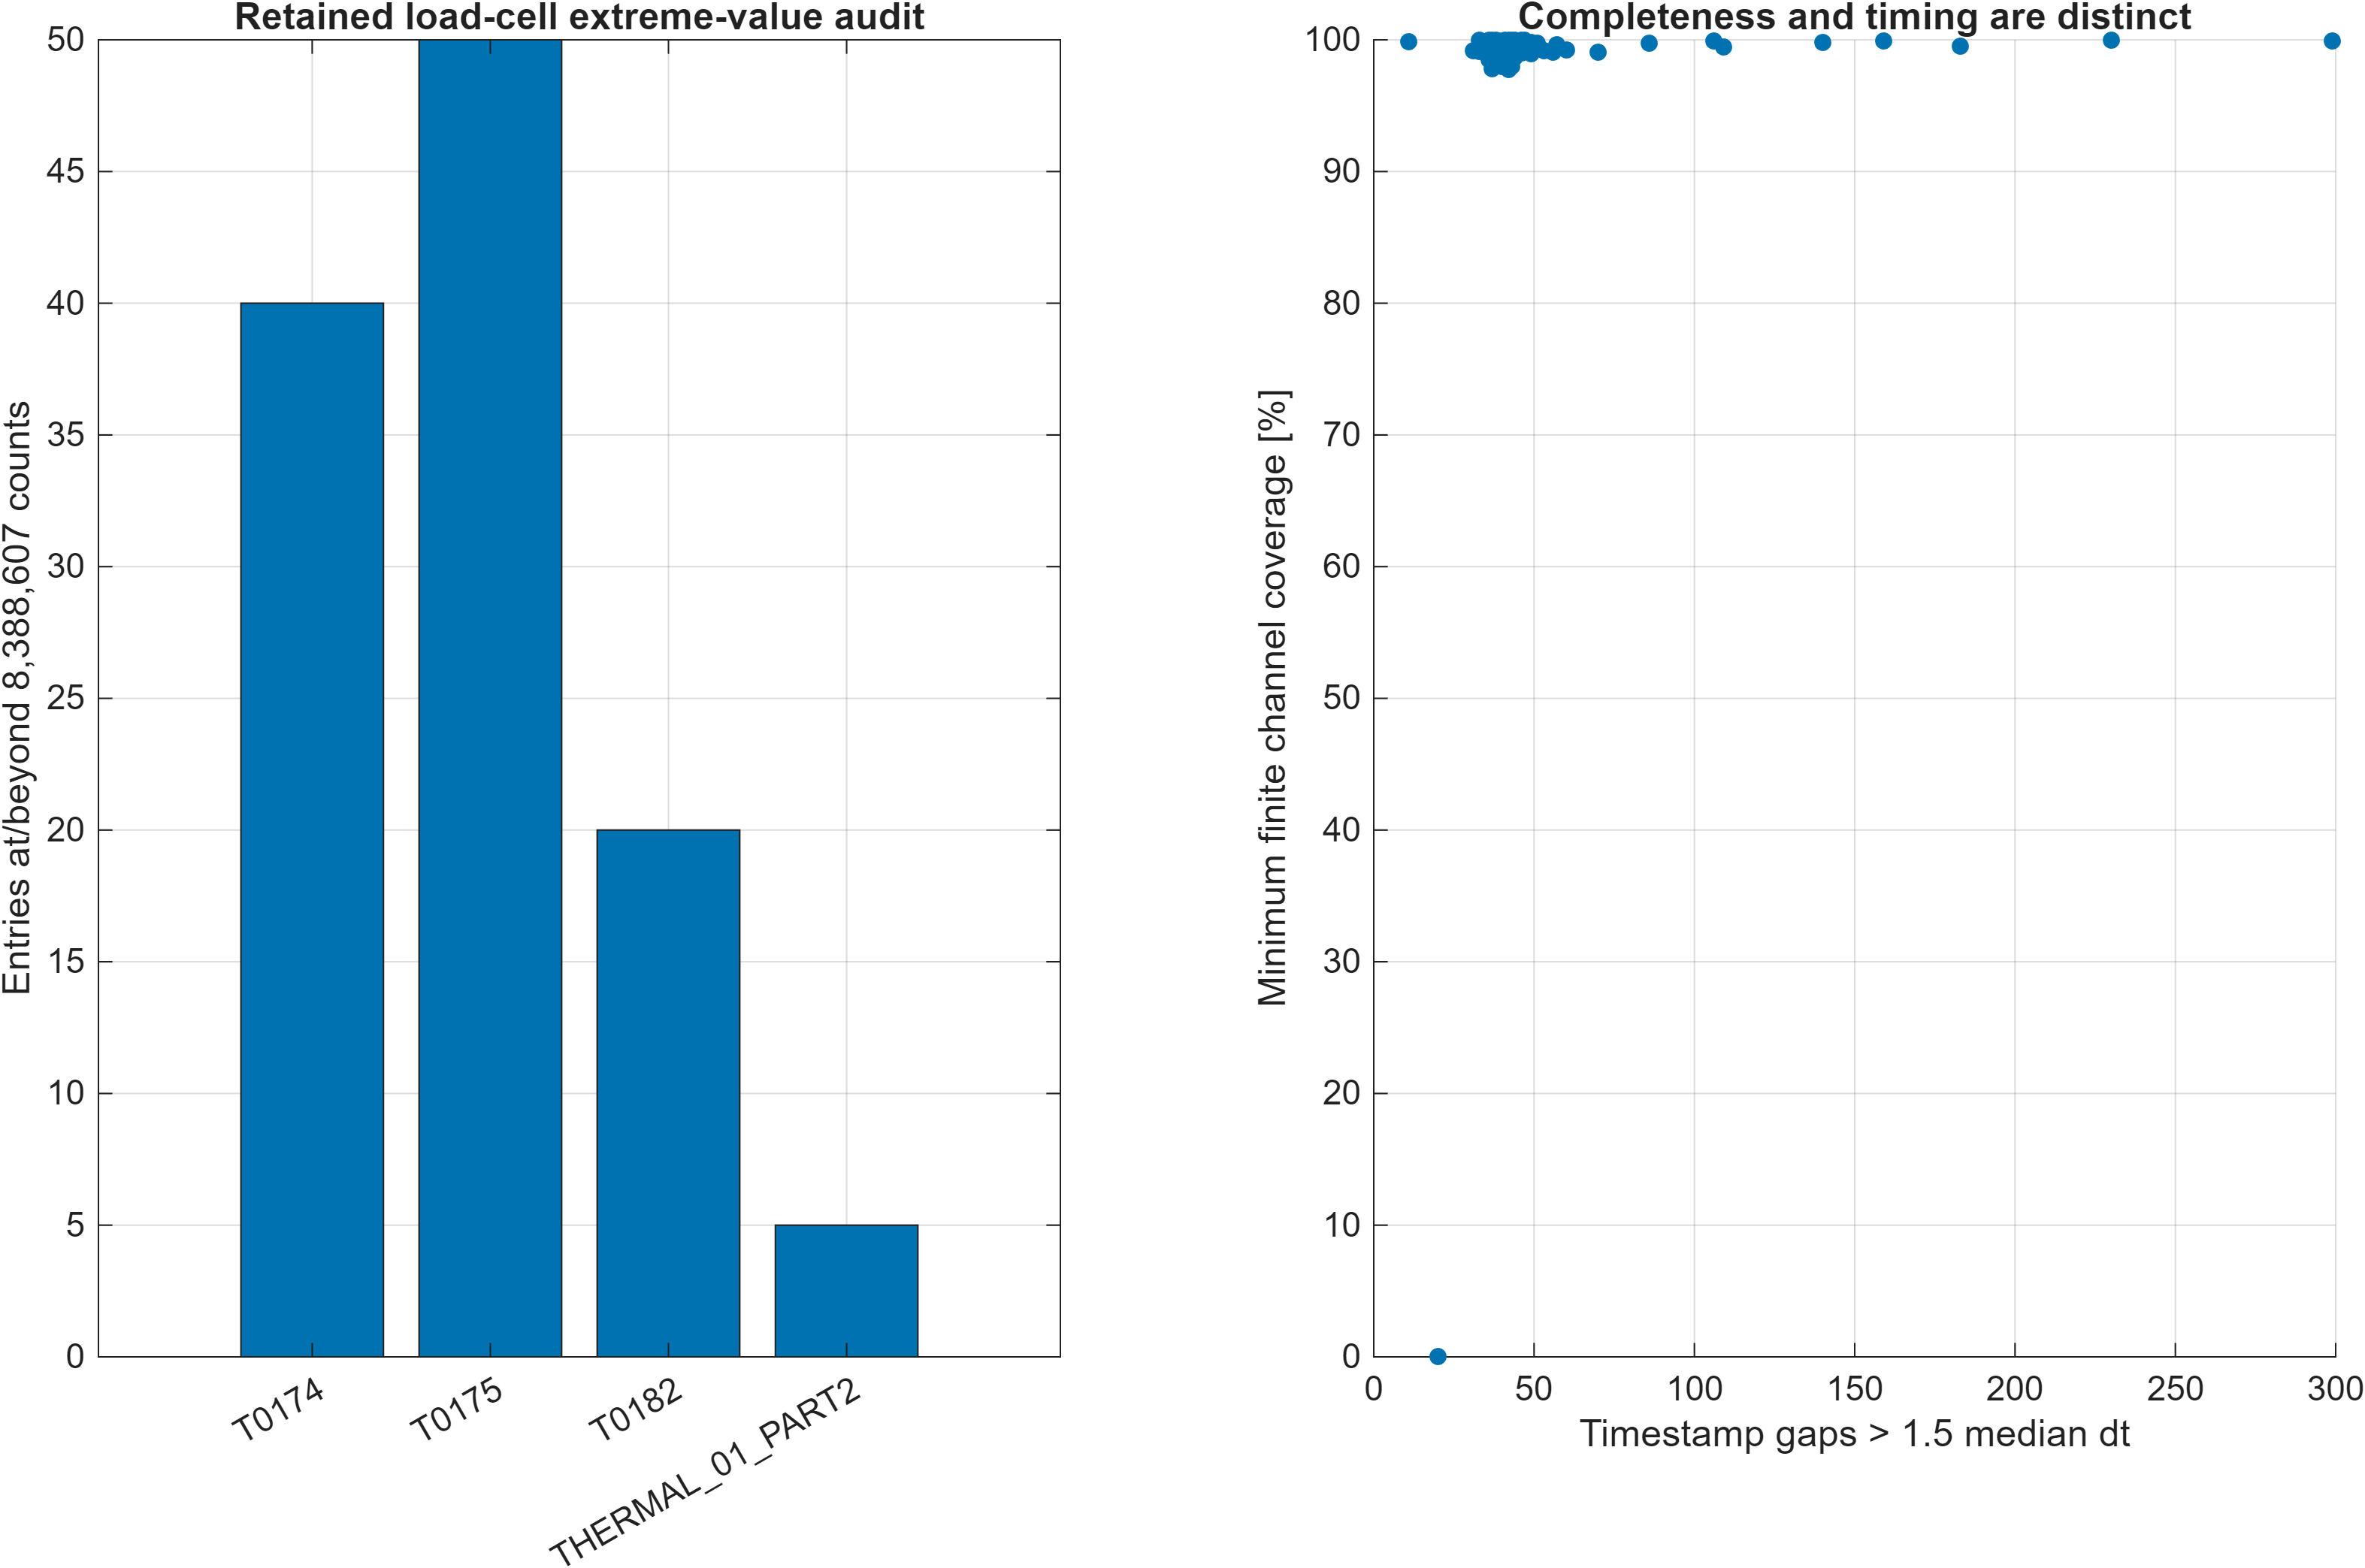
\includegraphics[width=\textwidth,height=0.37\textheight,keepaspectratio]{figures/F32_limitations_summary.png}
\caption{Data-quality issues retained in the cleaned data and disclosed for interpretation.}\label{fig:F32}
\end{figure}
The quality summary exposes two different risks: 115 load-cell entries in 4 recordings meet the extreme-value audit threshold, while every retained recording has timestamp gaps. The largest thermal left-cell value is 1e+07 times its run median, incompatible with treating a simple average as a representative baseline without investigation. Median summaries limit isolated-artifact influence but cannot restore lost dynamics or certify accuracy. High finite coverage and stable medians therefore do not remove the need for acquisition repair, calibration and sample-level cleaning provenance.\par

\Needspace{5\baselineskip}
\section{Data Limitations and Future Work}
All retained recordings have source QC warnings. Near-complete finite sensor coverage must not be mistaken for trustworthy timing or calibrated physical measurement. The following limitations should guide the next experimental campaign.

\begin{itemize}
\item Acquire hardware-timestamped data with verified units, a measured sampling clock, gap logging and an anti-aliasing strategy. Record sufficiently long uninterrupted vibration intervals.
\item Establish independent load-cell calibration, tare checks, sensor orientation and measurement uncertainty. Retained extreme values require review of acquisition and earlier cleaning before calibration or safety-related inference.
\item Preserve raw data and sample-level cleaning provenance. The current cleaned files do not identify which values were previously interpolated or spike-filtered. The present pipeline cannot reconstruct lost peaks.
\item Collect same-batch unloaded and loaded baselines, balanced repetitions and recorded temperatures. Use a tachometer or measured excitation channel to distinguish motor command from actual excitation.
\item Record disturbance triggers, wind speed and impact force before attempting damping, settling-time or frequency-response identification.
\item Repeat controlled thermal cycles with fixed load and excitation to test compensation on independent sessions. The two present thermal segments are one session, not a validation split.
\item Resolve duplicate and suspicious test identifiers using acquisition logs. Current traceability uses complete relative paths, preserving the existing identifiers.
\end{itemize}
The cleaned load-cell data retain 115 entries at or above an absolute magnitude of 8,388,607 counts in 4 recordings. The largest retained left-channel value is 7.97700158e+12 counts. This threshold is an audit flag motivated by the project HX711 acquisition code, not an automatic correction or a new source QC decision. Median summaries reduce the influence of isolated extreme entries on descriptive aggregates.

\Needspace{5\baselineskip}
\section{Conclusion}
Position sensitivity is the most consistent static finding: within each mass/batch stratum, moving the load right decreases the left-channel median and increases the right-channel median. Large offsets and unequal count sensitivities prevent interpreting these signals as forces. Static repetition scatter is small relative to raw output levels, but there is no specified acceptance tolerance and stable medians can conceal waveform artifacts.

Unloaded mean z RMS rises from 0.00544 to 0.01452 g between PWM 64 and 192, a factor of 2.67. Yet mean peak amplitude decreases 45.9 percent from PWM 128 to 192. Sustained vibration and isolated excursions therefore demand different model features. In the combined campaign, center loading has the lowest mean RMS in all nine matched mass/PWM comparisons, while mass and off/on effects are not uniformly monotonic. These observations motivate a model that accounts for interacting operating conditions, subject to independent replication.

The right load-cell thermal association is much stronger in the second segment (R-squared 0.992) than in the first (0.310), but the common time evolution and single session cannot establish causality or transferable compensation. Disturbance records contain localized peaks and, in some cases, sustained post-feature motion; missing forcing and event timing prevent damping identification. The recovered T0236 response peak at 1.3514 Hz lies in a broad low-frequency feature and is not a validated mode. Ninety of 91 candidate recordings still fail timing criteria.

The next experimental priority is calibrated, synchronized measurement with uninterrupted timestamps, measured excitation and disturbance triggers, matched baselines, and independent thermal sessions. Preserve sample-level cleaning provenance and resolve source identifiers before training. The present work supplies evidence and requirements for digital twin development; neither the bridge model nor a functioning digital twin has been validated.

\clearpage\section{Appendix: Figure and Dataset Index}
Stable identifiers F01--F32 refer to the original figures; the added spectrum is F33, placed with the frequency results. The self-contained report includes \texttt{plot\_manifest.csv} with full source paths, conditions, methods and discussions; \texttt{dataset\_index.csv} with run metrics; \texttt{frequency\_audit.csv} with eligibility decisions; and \texttt{analysis\_evidence.csv} with unrounded numerical discussion inputs. The FFT bins are supplied in \texttt{T0236\_fft\_spectrum.csv}. Source paths refer to the original dataset; compilation needs only the included images.

\fontsize{8.5}{9.5}\selectfont\renewcommand{\arraystretch}{1}\begin{longtable}{p{0.08\textwidth}p{0.73\textwidth}r}\toprule Figure & Image filename & Runs\\\midrule\endhead
F01 & \path{F01_experimental_categories.png} & 119\\
F02 & \path{F02_condition_counts.png} & 119\\
F03 & \path{F03_timing_distributions.png} & 119\\
F04 & \path{F04_sensor_coverage_qc.png} & 119\\
F05 & \path{F05_static_time_histories.png} & 3\\
F06 & \path{F06_static_mass_response.png} & 26\\
F07 & \path{F07_static_asymmetry.png} & 26\\
F08 & \path{F08_static_repeatability.png} & 26\\
F09 & \path{F09_position_response.png} & 26\\
F10 & \path{F10_position_asymmetry.png} & 26\\
F11 & \path{F11_relative_signal_distribution.png} & 26\\
F12 & \path{F12_vibration_time_histories.png} & 3\\
F13 & \path{F13_vibration_rms.png} & 9\\
F14 & \path{F14_vibration_peaks.png} & 9\\
F15 & \path{F15_vibration_axes.png} & 9\\
F16 & \path{F16_timestamp_integrity.png} & 91\\
F17 & \path{F17_spectral_eligibility.png} & 91\\
F18 & \path{F18_combined_rms_mass.png} & 60\\
F19 & \path{F19_combined_rms_position.png} & 60\\
F20 & \path{F20_combined_loadcell_histories.png} & 3\\
F21 & \path{F21_matched_vibration_off_on.png} & 29\\
F22 & \path{F22_thermal_temperature.png} & 2\\
F23 & \path{F23_thermal_loadcell_temperature.png} & 2\\
F24 & \path{F24_thermal_accel_temperature.png} & 2\\
F25 & \path{F25_thermal_elapsed_drift.png} & 2\\
F26 & \path{F26_thermal_sensitivity_summary.png} & 2\\
F27 & \path{F27_disturbance_transients.png} & 3\\
F28 & \path{F28_disturbance_metrics.png} & 6\\
F29 & \path{F29_impact_envelopes.png} & 3\\
F30 & \path{F30_combined_response_map.png} & 60\\
F31 & \path{F31_coverage_summary.png} & 119\\
F32 & \path{F32_limitations_summary.png} & 119\\
F33 & \path{F33_T0236_base_matlab_fft.png} & 1\\
\bottomrule\end{longtable}\normalsize
\subsection*{Thermal fitted associations}
Slopes use left temperature. Load-cell units are counts per degree Celsius; acceleration units are g per degree Celsius. These are descriptive fits, not correction coefficients.

\small\begin{longtable}{p{0.25\textwidth}p{0.30\textwidth}rr}\toprule Segment & Sensor & Slope & $R^2$\\\midrule\endhead
THERMAL\_01\_PART1 & loadcell\_left\_raw & -1411.7 & 0.018\\
THERMAL\_01\_PART1 & loadcell\_right\_raw & 1602.6 & 0.310\\
THERMAL\_01\_PART1 & accel\_x\_g & 0.00078244 & 0.477\\
THERMAL\_01\_PART1 & accel\_y\_g & 0.00032607 & 0.349\\
THERMAL\_01\_PART1 & accel\_z\_g & -0.00092083 & 0.038\\
THERMAL\_01\_PART2 & loadcell\_left\_raw & -159.97 & 0.328\\
THERMAL\_01\_PART2 & loadcell\_right\_raw & 3465.6 & 0.992\\
THERMAL\_01\_PART2 & accel\_x\_g & 0.0017698 & 0.697\\
THERMAL\_01\_PART2 & accel\_y\_g & 8.2876e-05 & 0.032\\
THERMAL\_01\_PART2 & accel\_z\_g & -0.00085522 & 0.274\\
\bottomrule\end{longtable}\normalsize
\clearpage\subsection*{Retained dataset index}
All source QC statuses are CHECK. Batch keys: W = October 9 wind/impact; L = September 18 static; V = September 18 vibration; F = September 18 frequency commands; C = September 25 combined/static; T = thermal. Repeated IDs remain distinct through full paths in the CSV index. A dash means unknown.

\noindent
\begin{minipage}[t]{0.48\textwidth}\vspace{0pt}\centering\fontsize{8.5}{9.6}\selectfont
\renewcommand{\arraystretch}{1}\begin{tabular}{lcrr}\toprule Test ID & Batch & kg & PWM\\\midrule
T0253 & W & 0 & 192\\
T0254 & W & 0 & 192\\
T0255 & W & 0 & 0\\
T0256 & W & 0 & 0\\
T0257 & W & 0 & 0\\
T0258 & W & 0 & 0\\
T0167 & L & 0.5 & 0\\
T0168 & L & 0.5 & 0\\
T0169 & L & 0.5 & 0\\
T0170 & L & 0.5 & 0\\
T0171 & L & 0.5 & 0\\
T0172 & L & 0.5 & 0\\
T0173 & L & 0.5 & 0\\
T0174 & L & 0.5 & 0\\
T0175 & L & 0.5 & 0\\
T0176 & L & 1 & 0\\
T0177 & L & 1 & 0\\
T0178 & L & 1 & 0\\
T0179 & L & 1 & 0\\
T0180 & L & 1 & 0\\
T0181 & L & 1 & 0\\
T0182 & L & 1 & 0\\
T0183 & L & 1 & 0\\
T0184 & L & 1 & 0\\
T0133 & V & 0 & 64\\
T0134 & V & 0 & 64\\
T0135 & V & 0 & 64\\
T0136 & V & 0 & 128\\
T0137 & V & 0 & 128\\
T0138 & V & 0 & 128\\
T0139 & V & 0 & 192\\
T0140 & V & 0 & 192\\
T0141 & V & 0 & 192\\
T0142 & F & 0 & 128\\
T0143 & F & 0 & 128\\
T0144 & F & 0 & 128\\
T0145 & F & 0 & 128\\
T0146 & F & 0 & 128\\
T0147 & F & 0 & 128\\
T0148 & F & 0 & 128\\
T0149 & F & 0 & 128\\
T0150 & F & 0 & 128\\
T0151 & F & 0 & 128\\
T0152 & F & 0 & 128\\
T0153 & F & 0 & 128\\
T0154 & F & 0 & 128\\
T0155 & F & 0 & 128\\
T0156 & F & 0 & 128\\
T0157 & F & 0 & 128\\
T0 & C & 1 & 192\\
T0194 & C & 0.25 & 64\\
T0195 & C & 0.25 & 64\\
T0196 & C & 0.25 & 64\\
T0197 & C & 0.25 & 128\\
T0198 & C & 0.25 & 128\\
T0199 & C & 0.25 & 128\\
T0200 & C & 0.25 & 192\\
T0201 & C & 0.25 & 192\\
T0202 & C & 0.25 & 192\\
T0203 & C & 0.5 & 64\\
\bottomrule\end{tabular}\end{minipage}
\hfill
\begin{minipage}[t]{0.48\textwidth}\vspace{0pt}\centering\fontsize{8.5}{9.6}\selectfont
\renewcommand{\arraystretch}{1}\begin{tabular}{lcrr}\toprule Test ID & Batch & kg & PWM\\\midrule
T0204 & C & 0.5 & 64\\
T0205 & C & 0.5 & 64\\
T0206 & C & 0.5 & 128\\
T0207 & C & 0.5 & 128\\
T0208 & C & 0.5 & 128\\
T0209 & C & 0.5 & 192\\
T0210 & C & 0.5 & 192\\
T0211 & C & 0.5 & 192\\
T0212 & C & 1 & 64\\
T0213 & C & 1 & 64\\
T0214 & C & 1 & 128\\
T0215 & C & 1 & 128\\
T0216 & C & 1 & 192\\
T0217 & C & 1 & 192\\
T0218 & C & 0.25 & 64\\
T0219 & C & 0.25 & 64\\
T0220 & C & 0.25 & 128\\
T0221 & C & 0.25 & 128\\
T0222 & C & 0.25 & 192\\
T0223 & C & 0.25 & 192\\
T0224 & C & 0.5 & 64\\
T0225 & C & 0.5 & 64\\
T0226 & C & 0.5 & 128\\
T0227 & C & 0.5 & 128\\
T0228 & C & 0.5 & 192\\
T0229 & C & 0.5 & 192\\
T0230 & C & 0.5 & 64\\
T0231 & C & 1 & 64\\
T0232 & C & 1 & 128\\
T0233 & C & 1 & 128\\
T0235 & C & 1 & 192\\
T0236 & C & 0.25 & 64\\
T0237 & C & 0.25 & 64\\
T0238 & C & 0.25 & 128\\
T0239 & C & 0.25 & 128\\
T0240 & C & 0.25 & 192\\
T0241 & C & 0.25 & 192\\
T0242 & C & 0.5 & 64\\
T0243 & C & 0.5 & 64\\
T0244 & C & 0.5 & 128\\
T0245 & C & 0.5 & 128\\
T0246 & C & 0.5 & 192\\
T0247 & C & 0.5 & 192\\
T0248 & C & 1 & 64\\
T0249 & C & 1 & 64\\
T0250 & C & 1 & 128\\
T0251 & C & 1 & 128\\
T0252 & C & 1 & 192\\
T0253 & C & 1 & 192\\
T0185 & C & 0.25 & 0\\
T0186 & C & 0.25 & 0\\
T0187 & C & 0.25 & 0\\
T0188 & C & 0.25 & 0\\
T0189 & C & 0.25 & 0\\
T0190 & C & 0.25 & 0\\
T0191 & C & 0.25 & 0\\
T0193 & C & 0.25 & 0\\
THERMAL\_01\_PART1 & T & -- & --\\
THERMAL\_01\_PART2 & T & -- & --\\
\bottomrule\end{tabular}\end{minipage}
\par\normalsize
\end{document}
